\documentclass[semcabeco,showtrims,trimframe,12pt,spreadimages,oneside]{memoir}
\usepackage[nexus]{../edlab}

\usepackage[pnld]{hedraoptions} %% << %%%%%%%%%%%%%%%%
\usepackage[baruch]{hedrastyles}
\usepackage[xetex,chicagofootnotes]{tipografia}
\usepackage[standart,compontinhos]{toc}
\usepackage{hedraextra}
\usepackage{penalidades}
\usepackage{graficos}
\usepackage{hedralogo}
\usepackage[shrink,siderepl]{hedrasides}
\usepackage{hifensextras}
\usepackage{fichatecnica}
\usepackage[standart]{aparatos}
\usepackage{tabelas}
\usepackage{versos}
%\usepackage{versos}
\usepackage{gitrevisioninfo}

\newcommand{\forceindent}{\leavevmode{\parindent=1,4em\indent}}


\makeatletter
\def\@xfootnote[#1]{%
  \protected@xdef\@thefnmark{#1}%
  \@footnotemark\@footnotetext}
\makeatother



\usepackage{footmisc}

\renewcommand*\footnoterule{}
%--------------------------------------------
\usepackage{afterpage}

\newcommand\blankpage{%
    \null
    \thispagestyle{empty}%
    \addtocounter{page}{0}%
    \newpage}


\setcounter{tocdepth}{1}
\setcounter{secnumdepth}{-2} 
\usepackage{commands}

\usepackage{setspace}

\makeatletter
\newenvironment{Parskip}{%
   \par
   \parskip=0.3\baselineskip \advance\parskip by 0pt plus 2pt
   \parindent=\z@
   \def\@listI{\leftmargin\leftmargini
      \topsep\z@ \parsep\parskip \itemsep\z@}
   \let\@listi\@listI
   \@listi
   \def\@listii{\leftmargin\leftmarginii
      \labelwidth\leftmarginii\advance\labelwidth-\labelsep
      \topsep\z@ \parsep\parskip \itemsep\z@}
   \def\@listiii{\leftmargin\leftmarginiii
       \labelwidth\leftmarginiii\advance\labelwidth-\labelsep
       \topsep\z@ \parsep\parskip \itemsep\z@}
   \partopsep=\z@
}{\par}
\makeatother

\makeatletter
\newenvironment{myParskip}{%
   \par
   \parskip=0.2\baselineskip \advance\parskip by 0pt plus 2pt
   \parindent=\z@
   \def\@listI{\leftmargin\leftmargini
      \topsep\z@ \parsep\parskip \itemsep\z@}
   \let\@listi\@listI
   \@listi
   \def\@listii{\leftmargin\leftmarginii
      \labelwidth\leftmarginii\advance\labelwidth-\labelsep
      \topsep\z@ \parsep\parskip \itemsep\z@}
   \def\@listiii{\leftmargin\leftmarginiii
       \labelwidth\leftmarginiii\advance\labelwidth-\labelsep
       \topsep\z@ \parsep\parskip \itemsep\z@}
   \partopsep=\z@
}{\par}
\makeatother

\newcommand{\mystar}{{\fontfamily{lmr}\selectfont$\star$}}

%------------------------------------------ INCLUIR EPIGRAFE EM PART
\let\oldafterpartskip\afterpartskip 

\newcommand\partepigraph[3][60pt]{
\renewcommand{\afterpartskip}{
\vskip#1
\epigraph{#2}{#3}
\vfil}
}
\newcommand\removeepigraph{
  \let\afterpartskip\oldafterpartskip}

\makeatletter
\renewenvironment{verse}
               {\let\\\@centercr
                \list{}{\itemsep      \z@
                        \itemindent   -1.5em%
                        \listparindent\itemindent
                        \rightmargin  \leftmargin
                        \advance\leftmargin 1.5em}%
                \item\relax}
               {\endlist}
\makeatother

\begin{document}

%%%!TEX root=./LIVRO.tex

\part{\textsc{mare nostrum: paranã tipi}}
\movetooddpage
\begin{absolutelynopagebreak}
\begin{vplace}
\begin{figure}[H]
\begin{adjustwidth}{-1.8cm}{}
  %\centering
  \vspace*{-2.6cm}
  %\hspace{-0.5cm}
  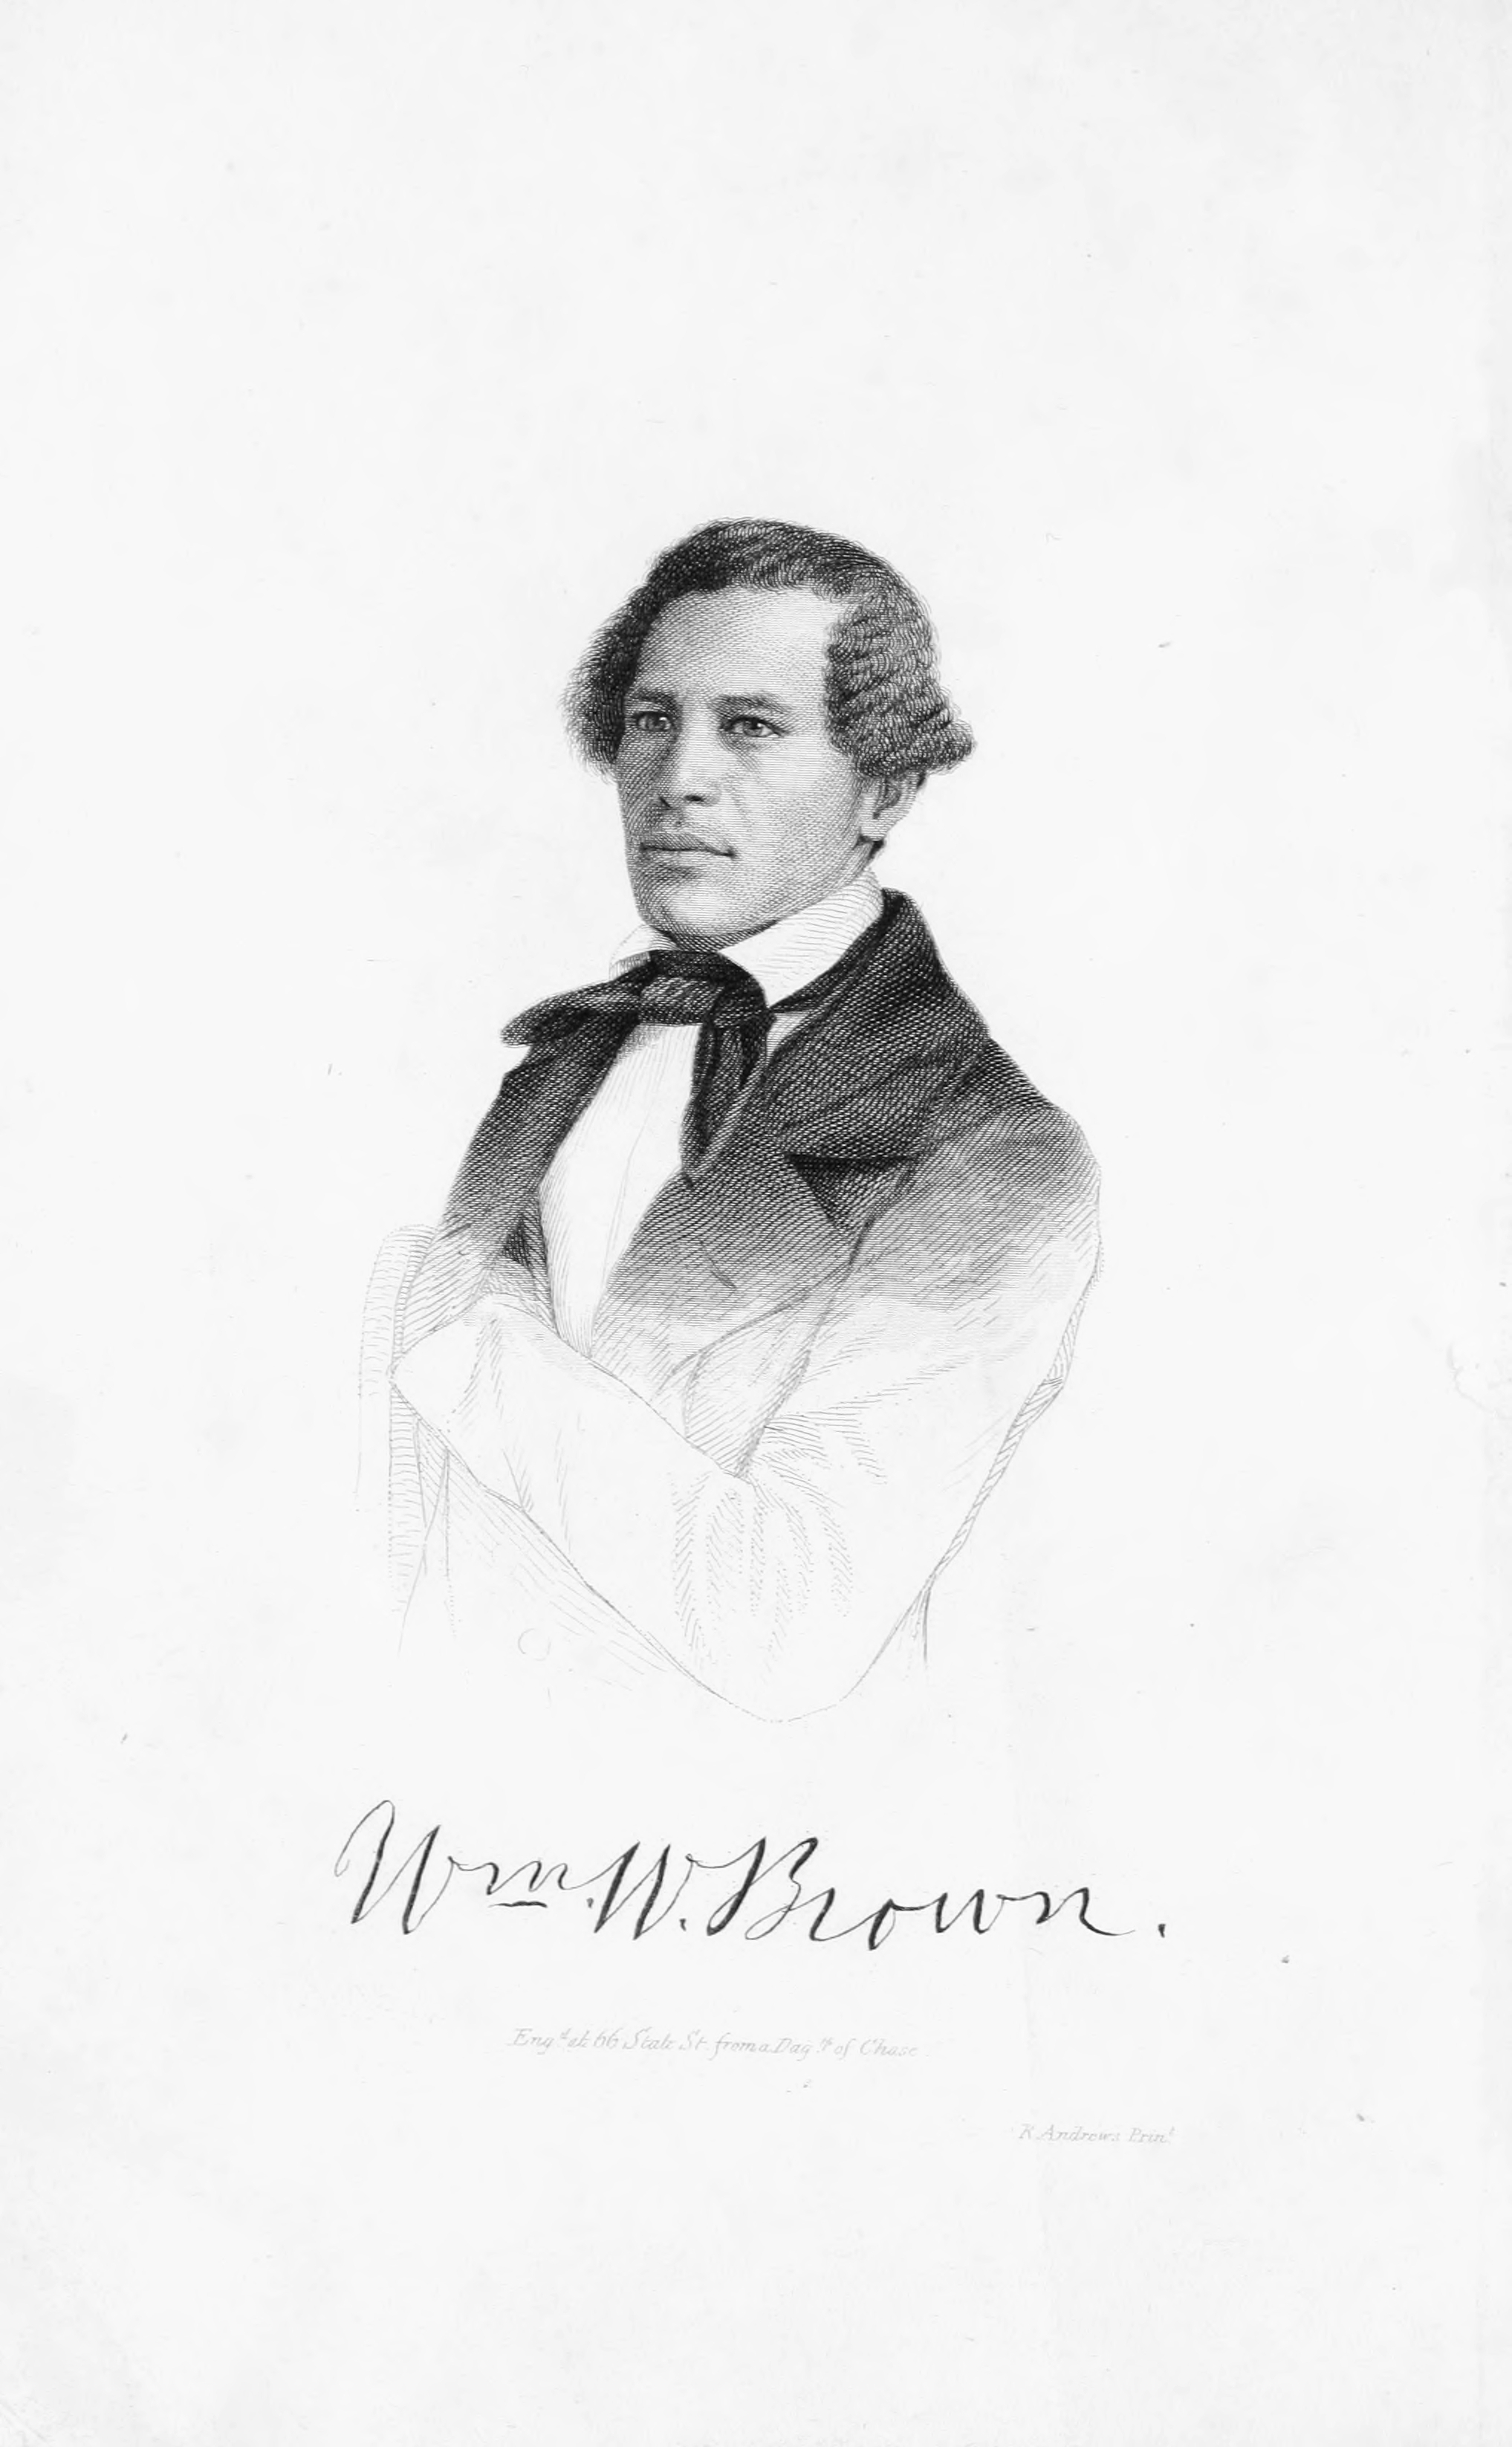
\includegraphics[width=134mm]{./imgs/front1.jpg}  \label{front}
  %\hfill
\end{adjustwidth}
  \caption{}
\end{figure}
\end{vplace}

\thispagestyle{empty}
\end{absolutelynopagebreak}


\pagebreak

\begin{absolutelynopagebreak}
\begin{vplace}
\begin{figure}[H]
\begin{adjustwidth}{-1.8cm}{}
  %\centering
  \vspace*{-2.6cm}
  %\hspace{-0.5cm}
  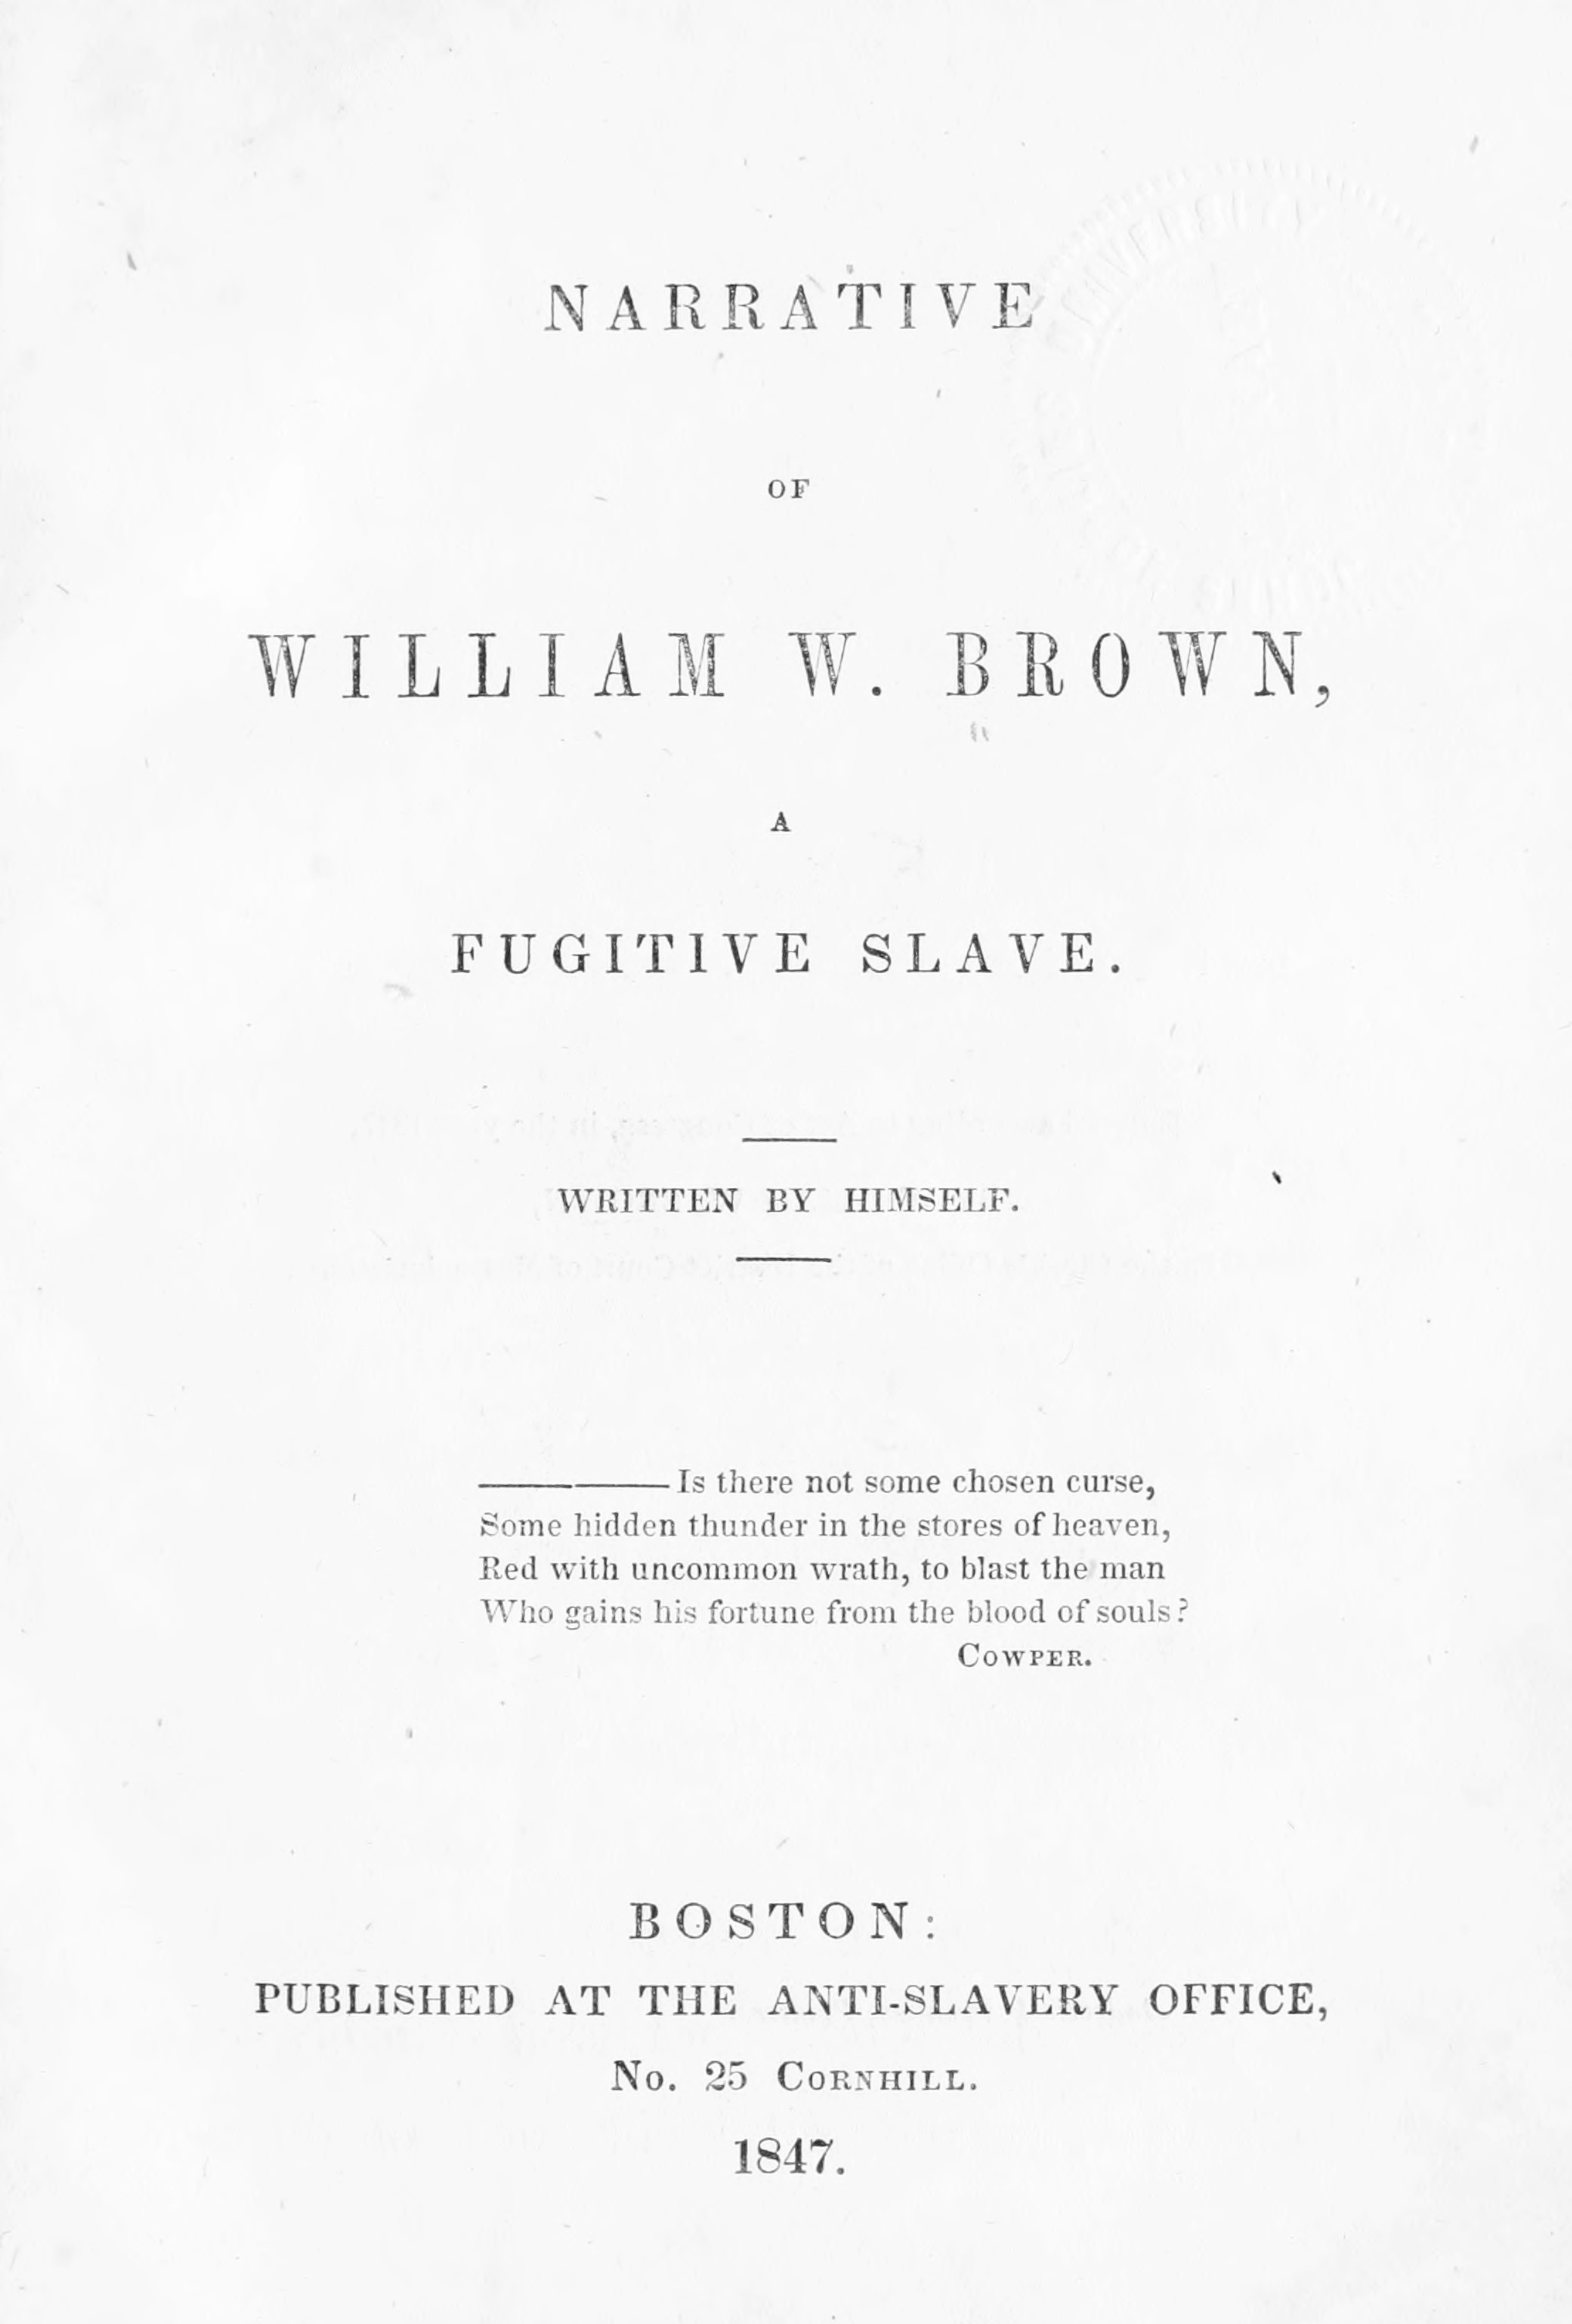
\includegraphics[width=134mm]{./imgs/front2.jpg}  
  %\hfill
\end{adjustwidth}
  \caption{Frontispício da primeira edição da autobiografia de William Wells Brown, publicada em Boston em 1847.}
\end{figure}
\end{vplace}

\thispagestyle{empty}
\end{absolutelynopagebreak}


\movetooddpage
\addcontentsline{toc}{part}{Narrativa de William Wells Brown}
\part*{Narrativa de William Wells Brown, escravo fugitivo, escrita por ele mesmo}


\chapter*{}
\thispagestyle{empty}
\begin{verse}
---Is there not some chosen curse,\\
Some hidden thunder in the stores of heaven,\\
Red with uncommon wrath, to blast the man\\
Who gains his fortune from the blood of \qb{}souls?\footnote{Tradução: ``Não haveria uma maldição seleta/ Um trovão oculto no arsenal celeste,/ Rubro com fúria especial, para fulminar o homem/ Que faz sua fortuna com o sangue das almas?''}
\end{verse}
\begin{flushright}
\versal{COWPER}\footnote{Brown atribui esses versos ao poeta inglês William
  Cowper (1731--1800). Na verdade, a passagem pertence à peça \emph{Cato,
  A Tragedy}, de Joseph Addison (1672--1719).}
\end{flushright}

\chapter{Para Wells Brown, de Ohio}

Treze anos atrás eu batia à sua porta, cansado, fugindo dos grilhões e
da chibata. Era forasteiro e você me hospedou. Estava faminto e você me
deu de comer. Estava nu e você me deu de vestir. A escravidão me negara
até um nome pelo qual pudesse ser chamado entre os homens, e você me deu
o seu. Eu seria uma criatura deveras vil se esquecesse tudo que te devo 
ou fizesse o que fosse para desonrar o seu nome sagrado!

Como pequeno testemunho da gratidão que tenho pelo meu primeiro
benfeitor, tomo a liberdade de lhe dedicar esta pequena \emph{Narrativa} dos
sofrimentos dos quais estava fugindo quando fui agraciado com a sua
compaixão. Entre as multidões que receberam seu auxílio, é bem possível
que você não se lembre de mim; mas até que eu esqueça Deus e a mim
mesmo, nunca me esquecerei de você.

Teu amigo agradecido

\begin{flushright}
\emph{William Wells Brown}
\end{flushright}

\chapter{Carta de Edmund Quincy} %, esq.

\begin{flushright}
\emph{Dedham, 1º de julho de 1847}
\end{flushright}

\begin{flushleft}
Para William Wells Brown
\end{flushleft}

Meu caro amigo: Agradeço sinceramente pelo privilégio de ler o
manuscrito da sua \emph{Narrativa}. Li"-a com profundo interesse e fiquei
emocionado. Tenho certeza que será, além de um enorme sucesso, de
extrema utilidade. Ela apresenta uma fase diferente do sistema
escravista infernal em relação àquela retratada na história admirável do
Sr.\,Douglass\footnote{Frederick Douglass (1819--1895): Abolicionista,
  jornalista e político americano. Sua primeira autobiografia, a
  \emph{Narrativa da vida de Frederick Douglass, um escravo americano},
  foi um sucesso de vendas na época e ainda é considerada um clássico da
  literatura dos \versal{EUA}.} e nos permite vislumbrar as crueldades atrozes de
outras partes do seu domínio.

As oportunidades que você teve de observar o funcionamento desse sistema
maldito foram particularmente grandes. Suas experiências na Lavoura, na
Casa Grande e, especialmente, no Rio, a serviço de Walker, o traficante
de escravos, quase não encontra paralelo entre outros indivíduos, e
certamente nenhum que tenha demonstrado a competência para descrevê"-los.
O que admiro, e o que me assombra, na sua \emph{Narrativa} é a calma e a
simplicidade com que descreve cenas e ações que poderiam muito bem
``levar as próprias pedras a se erguerem em motim'' contra a Instituição
Nacional que as tornam possíveis.

Como irá perceber, em muito pouco fiz uso da gentil permissão que me deu
para alterar aquilo que escreveras. Corrigir alguns equívocos, que \label{ref1}
pareciam ser meros erros de cópia, cometidos na pressa da composição,
empreendida em condições desfavoráveis, e sugerir alguns abreviamentos,
foi tudo que ousei fazer. Seria muita audácia da minha parte, e muita
vaidade também, tentar melhorar as descrições do que você viu e sofreu.
Algumas das cenas fariam jus ao próprio De Foe.

Confio que sua narrativa terá ampla circulação e tenho certeza de que
ela o merece. Deve possuir uma natureza diferente da minha o homem que
encerre a leitura da \emph{Narrativa} sem acreditar que entende a escravidão
melhor do que nunca, e a odeie ainda mais.

Fiel e respeitosamente, 

Seu amigo

\begin{flushright}
\emph{Edmund Quincy}
\end{flushright}

\chapter{Prefácio à primeira edição}

Os amigos da liberdade podem comemorar o surgimento da \emph{Narrativa} a
seguir, que acrescenta mais um volume à crescente literatura
antiescravista contemporânea. Como afirmou um grande observador da
natureza humana: ``Deixem"-me compor as canções de uma nação e não me
importarei com quem compõe suas leis'';\footnote{Frase de Andrew Fletcher
  (1655--1716), escritor e político antiunionista escocês.} e com o
mesmo grau de verdade pode"-se dizer que, entre um povo leitor como o
nosso, nossos livros irão ao menos caracterizar nossas leis. É uma
influência que avança silenciosamente em sua missão, mas jamais deixa de
encontrar o caminho a muitos corações calorosos para acender em seus
altares a chama da liberdade que um dia se conflagrará no incêndio que
há de consumir a opressão.

Este livreto é uma voz emanando da prisão, desvendando os feitos
sombrios que nela são perpetrados. Nossa causa recebe um grande socorro
dessa fonte. Os nomes daqueles que vieram de lá, e que batalharam
valorosamente pela justiça, não precisam ser registrados aqui. As obras
de alguns deles são monumentos eternos à divindade e seu registro
perpétuo encontra espaço nos corações agradecidos dos cativos redimidos.

Poucas pessoas tiveram maior oportunidade para conhecer a escravidão em
todos os seus aspectos mais terríveis do que William W. Brown. Ele
esteve por trás dos panos. Visitou suas câmaras secretas. Os ferros dela
penetraram a sua alma. Os laços mais caros da natureza foram fendidos em
sua pessoa. Uma mãe foi açoitada cruelmente perante seus próprios olhos.
Um pai\ldots{} mas, ah, escravo não tem pai. Um irmão se tornou vítima
de sua própria misericórdia. Uma irmã foi entregue ao controle
irresponsável do pálido opressor. E esta nação assente com a cena. A
União americana sanciona esses feitos. A Constituição protege os
criminosos. A religião americana santifica o crime. Mas a maré está
virando. Uma corrente submarina arrasta o país para a frente. Uma voz de
alerta, de admoestação, de censura, de rogo, está soando. Mãos seguram
mãos e corações se mesclam com corações na grande obra da salvação dos
escravos.

Mesmo agora, as convulsões do monstro evidenciam suas feridas profundas.

O autor desta \emph{Narrativa} foi emprestado pelo seu senhor para um
``\emph{traficante de almas}'' e testemunhou todos os horrores do
tráfico, desde a compra do rebanho humano nos estados criadores de
escravos, que produzem uma cena constante da separação das vítimas dos
seus entes queridos, até a sua venda final no mercado do Sul, para serem
exauridos em sete anos ou entregues à luxúria dos \emph{cristãos}
sulistas.

Muitas cenas pungentes são retratadas explicitamente, mas também com uma
simplicidade e uma engenhosidade que transmitem a certeza sobre a
veracidade da imagem.

Este livro fará muito para desmascarar aqueles que ``se vestiram com o
libré da corte celestial'' a fim de disfarçar a monstruosidade dos seus
atos.

Durante os últimos três anos, o autor dedicou todas as suas energias à
causa antiescravista. Labutando sob todas as deficiências e desvantagens
decorrentes de ter sido educado sob a escravidão, de ter sido sujeitado,
como foi desde nascença, a todos os males e privações inerentes à sua
condição, ainda assim ele seguiu em frente, atraído ao trabalho pelo
amor à liberdade, estimulado pela memória do próprio sofrimento, instado
pela consideração de que mãe, irmãos e irmã ainda agonizavam no
cativeiro ao lado de três milhões de filhos do Nosso Pai, sustentado por
uma fé inabalável na onipotência da verdade e no triunfo final da
justiça, para defender a causa dos escravos, e pela eloquência da sua
sinceridade transmitiu a certeza a muitas mentes e arregimentou a
simpatia e a cooperação de muitos outros em prol da causa.

Seu trabalho se limitou principalmente ao oeste do estado de Nova York,
onde conquistou muitos amigos queridos com seu zelo incansável, sua
energia perseverante, sua fidelidade constante e sua bondade universal.

Leitor, és um abolicionista? O que fizestes pelo escravo? O que fazes
por ele? O que pretendes fazer? Uma grande obra nos espera. Quem há de
ficar parado? Em termos comparativos, este é o grande movimento
humanitário da nossa era, engolindo, por ora, todas as outras questões.
O curso da história humana, obediente às leis imutáveis da nossa
existência, avança rapidamente para uma crise final. Eis a pergunta:

\begin{verse}
Have ye chosen, O my people, on whose \qb{}party ye shall stand,\\
Ere the Doom from its worn sandal shakes \qb{}the dust against our land?\footnote{Tradução: ``Já escolhestes, ó, meu povo, que partido ireis tomar,/ Antes que o Destino de suas sandálias gastas sacuda a poeira contra a
nossa terra?''. Versos de \emph{The Present Crisis}, do poeta
  romântico americano James Russell Lowell (1819--1891). ``Sacudir a
  poeira'' é uma referência a Mateus 10:14 e à antiga prática judaica de
  sacudir a poeira dos pés ao sair de cidades não"-judaicas para indicar
  separação do mundo gentio.}
\end{verse}

Você é cristão? Esta é a realização do Cristianismo prático, e não há
outra forma. O Cristianismo é \emph{prático} em sua própria essência e
natureza. É uma vida que nasce da alma imbuída com o seu espírito. É
amigo da causa missionária? Este é o maior empreendimento missionário de
hoje. Três milhões de \emph{cristãos}, transformados em pagãos pela lei,
anseiam pelas boas novas do Evangelho da liberdade. É amigo da Bíblia?
Vem, então, e nos ajuda a restaurar a vista para esses milhões cujos
olhos foram furados pela escravidão, para que possam enxergar e ler a
Bíblia. Ama Deus, a quem nunca viu? Então manifesta esse amor e devolve
ao irmão que já vistes a sua legítima herança, da qual foi privado por
tanto tempo e com tanta crueldade.

Não é por uma única geração de três milhões que trabalhamos, por mais
sublime que seja tal esforço. É pela humanidade, ao redor do mundo, não só agora, mas por todos os tempos, e por todas as gerações futuras:

\begin{verse}
For he who settles Freedom's principles,\\
Writes the death"-warrant of all tyranny.\footnote{Tradução: ``Pois quem estabelece os princípios da Liberdade/ Redige a sentença de morte
de toda a tirana.'' De \emph{L'Envoi}, poema final de \emph{A
  Year's Life}, o primeiro livro de James Russell Lowell.}
\end{verse}

É um trabalho vasto, um empreendimento glorioso, digno da devoção
inarredável de toda a vida dos grandes e dos bons.

O escravismo e os escravistas devem ser convertidos em seres
ignominiosos e detestáveis. Devem perder sua respeitabilidade e sua
reputação cristã. Devem ser tratados como ``ladrões de homens, culpados
do mais grave roubo e pecadores de primeira ordem''.\footnote{Passagem da
  Disciplina da Igreja Presbiteriana dos \versal{EUA}, adotada em 1794 e
  eliminada em 1816 com a influência crescente dos escravistas na
  Assembleia Geral.} Seus cúmplices mais culpados, na pessoa dos
\emph{apologistas nortistas}, tanto na Igreja quanto no Estado, devem
ser colocados na mesma categoria. Os homens honestos devem ser
convencidos a ver esses crimes com a mesma aversão e desprezo que
destinam aos ladrões e assassinos menos culpados, até que:


\begin{verse}
The common damned shun their society,\\
And look upon themselves as fiends less \qb{}foul.\footnote{Tradução: ``Os condenados comuns rejeitam a sua sociedade/ E se consideram demônios menos atrozes.'' De \emph{The Grave}, do poeta
  escocês Robert Blair (1699--1746).}
\end{verse}

Quando o crime da escravidão receber sua justa sentença, o trabalho
estará completo. E terá chegado o dia glorioso:

\begin{verse}
When man nor woman in all our wide \qb{}domain,\\
Shall buy, or sell, or hold, or be a slave.\footnote{Tradução: ``Quando nem homem nem mulher em nossos vastos domínios/ Há de comprar, ou vender, ou ter, ou ser escravo.'' Paráfrase dos versos finais de \emph{Inscription under the Picture of an Aged Negro"-woman}, do poeta escocês James Montgomery (1771--1854).}
\end{verse}

\bigskip

\begin{flushright}
\emph{J. C. Hathaway}

Farmington, Nova York, 1847.
\end{flushright}



\chapter*{Capítulo I}
\addcontentsline{toc}{chapter}{Capítulo \textsc{i}}

Nasci em Lexington, Kentucky. O homem que me roubou assim que nasci \label{ref5}
registrava o nascimento de todos os bebês que alegava serem de sua
propriedade em um livro que mantinha para esse fim. O nome de minha mãe
era Elizabeth. Ela teve sete filhos, a saber: Solomon, Leander,
Benjamin, Joseph, Millford, Elizabeth e eu. Nenhum de nós tinha o mesmo
pai que o outro. O nome de meu pai, como soube de minha mãe, era George
Higgins. Ele era um homem branco, aparentado com meu senhor, e ligado a
algumas das famílias mais proeminentes do Kentucky.

Meu senhor possuía cerca de quarenta escravos, vinte e cinco dos quais
eram lavradores. Ele se mudou do Kentucky para o Missouri quando eu era
ainda muito jovem e se estabeleceu cinquenta ou setenta quilômetros
acima de St.\,Charles, no Rio Missouri, onde, além da clínica de
medicina, praticava a moagem de cereais, o comércio e a agricultura. Ele
tinha uma fazenda grande, e seus principais produtos eram o tabaco e o
cânhamo. As senzalas ficavam situadas nos fundos da fazenda, com a casa
do feitor, chamado Grove Cook, em seu meio. Ele era encarregado de toda
a fazenda e, por não ter família, mantinha uma mulher que cuidava da
casa para ele; era ela a responsável por distribuir as provisões para os
lavradores.

Também havia uma mulher que ficava nos alojamentos para cozinhar para os
trabalhadores do eito, que eram convocados para a sua labuta incessante
todos os dias às quatro da manhã. O sino pendurado em um poste junto à
casa do feitor repicava e então eles tinham meia hora para fazer seu
desjejum e partir para o campo. Às quatro e meia, o feitor soava um
berrante, sinalizando o começo do trabalho, e todos que não estivessem
presentes naquele instante recebiam dez chibatadas do chicote com o qual
o feitor estava sempre armado. O cabo tinha quase um metro de
comprimento, com a ponta cheia de chumbo, e a chibata de couro tinha
dois metros, com arame trançado na ponta. O chicote era aplicado com
bastante frequência e liberdade, e qualquer pequeno delito por parte de
um escravo era causa para a sua utilização. Durante a época em que o Sr.\,Cook foi feitor, eu era criado doméstico, uma situação preferível à do
escravo do eito, pois eu era mais bem alimentado, me vestia melhor e não
era forçado a me levantar com o tocar do sino, e sim cerca de meia hora
depois. Muitas vezes fiquei deitado, escutando os estalos da chibata e
os berros dos escravos. Minha mãe trabalhava no eito e, uma manhã,
chegou ao campo dez ou quinze minutos depois dos outros. Logo que chegou
no local onde eles iriam trabalhar, o feitor começou a açoitá"-la.

--- Ah! por favor\ldots{} Ah! por favor\ldots{} Ah! por favor --- ela
gritava.

Essas eram as palavras recorrentes dos escravos, implorando por piedade
das mãos dos seus opressores. Eu reconheci a voz dela, saltei do meu
catre e saí correndo para a porta. A lavoura ficava longe da casa, mas
ainda assim eu escutava cada estalo do chicote, cada grito e gemido da
minha pobre mãe. Permaneci junto à porta, sem ousar ir além. Senti um
calafrio correr de cima a baixo e caí em prantos. Após a décima
chibatada, o som do chicote cessou e eu voltei para a cama, consolado
apenas pelas lágrimas. O sol ainda não havia nascido.

\chapter*{Capítulo II}
\addcontentsline{toc}{chapter}{Capítulo \textsc{ii}}

Meu senhor era um demagogo político e logo encontrou quem estivesse
disposto a obter"-lhe um cargo em troca dos favores que poderia prestar,
e poucos anos após sua chegada ao Missouri ele foi eleito para o
Legislativo estadual. Enquanto ele estava ausente, o Sr.\,Cook, o feitor,
ficava encarregado de tudo, e logo se tornou ainda mais tirânico e
cruel. Entre os escravos da fazenda havia um que atendia pelo nome de
Randall. Era um homem de cerca de um metro e oitenta de altura, esbelto,
conhecido por todos por sua enorme força, e considerado o escravo mais
valioso e capaz de toda a plantação; contudo, por melhor ou mais útil
que seja um escravo, ele quase nunca escapa da chibata. Mas Randall era
uma exceção. Ele estava na fazenda desde que eu me lembrava, mas eu
nunca o vira ser castigado. Isso não era graças ao senhor ou ao feitor.
Muitas vezes eu o ouvi declarar que nenhum branco jamais o açoitaria,
que morreria antes disso.

Desde o dia em que chegara à fazenda, Cook sempre declarara que podia e
iria castigar qualquer crioulo que trabalhasse sob o seu comando no
campo. Meu senhor lhe dissera inúmeras vezes que não tentasse açoitar
Randall, mas o feitor estava decidido. Assim que se tornou o único
ditador da fazenda, determinou que chegara o momento de executar suas
ameaças. Um dia, ordenou uma tarefa muito difícil, mais do que Randall
seria capaz de fazer; e à noite, como a tarefa não estava concluída,
disse a Randall que deveria lembrar dele na manhã seguinte. No outro
dia, depois que os escravos haviam feito seu desjejum, Cook chamou
Randall e disse que pretendia açoitá"-lo. O feitor ordenou que ele
cruzasse as mãos e fosse amarrado. Randall perguntou por que queria
açoitá"-lo. A resposta foi que ele não completara a tarefa do dia
anterior. Randall disse que a tarefa era grande demais, e que a teria
realizado se não fosse por isso. Cook respondeu que não fazia diferença,
que era preciso açoitá"-lo. Randall ficou em silêncio por um instante e
então respondeu:

--- Sr.\,Cook, eu sempre tentei agradá"-lo desde que o senhor chegou à
fazenda, mas o senhor está decidido a não se satisfazer com o meu
trabalho. Deixe"-me trabalhar como posso. Homem nenhum colocou as mãos em
mim para me açoitar nos últimos dez anos, e há muito concluí que não
existe homem vivo que vá me açoitar.

Cook, percebendo pelo olhar e os gestos decididos de Randall que este
iria resistir, chamou três escravos que estavam trabalhando, ordenou
que agarrassem Randall e o amarrassem. Os escravos ficaram parados; eles
conheciam Randall, e sabiam muito bem a força deste, então tinham medo
de atacá"-lo. Logo que Cook ordenou que os homens o agarrassem, Randall
se virou para eles e disse:

--- Rapazes, vocês todos me conhecem, sabem que posso com qualquer de
vocês três e que o homem que encostar em mim há de morrer. Esse branco
não consegue me castigar sozinho, então chamou vocês para ajudá"-lo.

O feitor não conseguiu convencê"-los a amarrar Randall e finalmente
ordenou que todos voltassem para o trabalho.

Randall não ouviu nada do feitor por mais de uma semana. Uma manhã, no
entanto, enquanto os escravos estavam no eito, ele chegou com três
amigos, Thompson, Woodbridge e Jones. Eles foram até onde Randall estava
trabalhando e Cook ordenou que deixasse o trabalho de lado e os
acompanhasse até o celeiro. Randall se recusou, então foi atacado pelo
feitor e seus companheiros; ele reagiu e os derrotou um a um,
prostrando"-os no chão. Woodbridge sacou sua pistola e disparou,
derrubando"-o com uma bala. Os outros saltaram sobre ele, desferindo
porretadas sobre a cabeça e no rosto até que conseguiram amarrá"-lo.
Depois, Randall foi levado ao celeiro e amarrado a uma trave. Cook lhe
deu mais de cem chibatadas com um chicote de couro pesado, mandou lavar
as feridas com salmoura e deixou"-o amarrado durante o dia. No dia
seguinte, ele foi desamarrado e levado à ferraria, onde uma bola com
corrente foi presa à sua perna. Randall foi forçado a trabalhar no campo
e completar a mesma quantidade de trabalho que todos os outros. Quando
voltou para casa, seu senhor ficou muito contente em descobrir que
Randall fora domado na sua ausência.

\chapter*{Capítulo III}
\addcontentsline{toc}{chapter}{Capítulo \textsc{iii}}

Pouco depois, meu senhor se mudou para a cidade de St.\,Louis e comprou
uma fazenda a seis quilômetros de distância, que colocou sob a
supervisão de um feitor chamado Friend Haskell, um típico yankee da Nova
Inglaterra. Os yankees são famosos por darem os feitores mais cruéis de
todos.

Minha mãe foi alugada na cidade, e eu também fui alugado lá pelo Major
Freeland, que mantinha uma taverna. Oriundo da Virgínia, ele estava
envolvido com corridas de cavalo, rinhas de galos e jogos de azar e era
um bêbado inveterado. Havia dez ou doze criados na casa e, quando ele
estava presente, o lugar era uma balbúrdia e um pandemônio. Em seus
acessos de fúria, ele atirava cadeiras nos criados; em seus momentos
mais racionais, quando desejava castigar alguém, os amarrava e açoitava
no defumadouro, então acendia uma fogueira com talos de tabaco para
defumá"-los. Isso que ele chamava de uma ``\emph{virginiada}''.

Reclamei para o meu senhor do tratamento que recebia do Major Freeland,
mas não fez diferença. Ele não dava nenhuma importância a isso, desde
que recebesse o dinheiro pelo meu trabalho. Após morar com o Major \enlargethispage{\baselineskip}
Freeland por cinco ou seis meses, fugi e me escondi na floresta perto da
cidade. Quando a noite caiu, me dirigi à fazenda do meu senhor, mas tive
medo de ser avistado, sabendo que se o feitor, o Sr.\,Haskell, me
achasse, eu seria arrastado de volta para o Major Freeland; assim,
permaneci na floresta. Um dia, enquanto estava na floresta, ouvi cães
ladrando e uivando, e logo eles se aproximaram tanto que reconheci os
sabujos do Major Benjamin O'Fallon, que criava cinco ou seis cães para
caçar escravos fugitivos.

Logo que me convenci de que eram eles, soube que a fuga seria
impossível. Encontrei refúgio na copa de uma árvore e os cães logo a
cercaram, e ali permaneceram até os caçadores chegarem, meia hora ou
três quartos de hora depois. Dois homens acompanhavam os cães e, assim
que chegaram, me mandaram descer. Eu desci e fui amarrado e levado à
cadeia de St.\,Louis. O Major Freeland logo apareceu, me soltou e ordenou
que eu o seguisse, o que fiz. Após voltarmos para casa, ele me amarrou
no defumadouro e eu fui açoitado horrivelmente. Após o Major me castigar
até se dar por satisfeito, ele mandou chamar Robert, seu filho, um jovem
de dezoito ou vinte anos, para garantir que eu fosse defumado. Ele
acendeu uma fogueira com talos de tabaco que logo me deixou tossindo e
espirrando. Esse era o modo como seu pai lidava com seus escravos na
Virgínia, Robert me contou. Após aplicarem o que consideravam uma
defumada decente, fui desamarrado e colocado no trabalho mais uma vez.

Robert Freeland era ``filho de peixe''. Apesar de muito jovem,
frequentemente chegava em casa embriagado. Creio que hoje ele é o
comandante popular de um barco a vapor no rio Mississippi. Os negócios
do Major Freeland logo decaíram e eu fui colocado a bordo do vapor
\emph{Missouri}, que fazia a rota entre St.\,Louis e Galena. O comandante
do navio era William B. Culver. Permaneci a bordo durante a temporada de
navegação, a época mais agradável que havia vivenciado até então. Ao
final do período, fui alugado pelo Sr.\,John Colburn, que mantinha o
Missouri Hotel. Ele era oriundo de um dos Estados Livres, mas não acho
que jamais pôs os pés nesta terra de Deus um inimigo mais inveterado dos
negros. Na época, o hotel era um dos maiores da cidade e empregava vinte
ou trinta criados, quase todos escravos.

O Sr.\,Colburn era muito perverso, e não apenas com os criados, mas com a
esposa também, uma excelente mulher e uma pessoa da qual nunca observei
um criado receber uma única palavra de rispidez, assim como nunca
observei uma palavra de gentileza do marido. Entre os escravos
empregados no hotel havia um chamado Aaron, que pertencia ao Sr.\,John F.
Darby, um advogado. Aaron lavava as facas. Um dia, uma das facas foi
colocada à mesa menos limpa do que poderia estar. Por essa ofensa, o Sr.\,Colburn atou Aaron no depósito de lenha e lhe deu cinquenta chibatadas
nas costas nuas com um chicote de couro, e depois me fez lavar Aaron com
rum. Isso pareceu deixá"-lo em mais agonia do que as vergastadas. Depois
que foi desamarrado, ele voltou para a casa do seu senhor e reclamou do
tratamento que recebera. O Sr.\,Darby também não deu nenhuma atenção ao
que ele tinha a dizer e o mandou de volta na mesma hora. Colburn, ao
descobrir que Aaron fora reclamar para o seu senhor, o amarrou de novo e
o castigou pior do que antes. As costas do pobre rapaz foram
literalmente cortadas em pedacinhos, tanto que não teve como trabalhar
pelos próximos dez ou doze dias.

Entre os criados havia também uma menina de nome Patsey cujo senhor
morava no campo. Uma noite, o Sr.\,Colburn a amarrou e açoitou até que
vários dos hóspedes apareceram para implorar que ele parasse. O motivo
para o castigo era o seguinte. Ela estava noiva de um homem que
pertencia ao Major William Christy, que residia seis ou sete quilômetros
ao norte da cidade. O Sr.\,Colburn a proibira de ver John Christy.
Supostamente, o motivo era o apreço que ele mesmo tinha por Patsey. Ela
foi encontrá"-lo naquela tarde e John voltou para casa com ela. O Sr.\,Colburn pretendia castigar John se ele passasse pelo cercado, mas este
conhecia muito bem o temperamento do rival e se manteve a uma distância
segura. Assim, ele extraiu sua vingança da pobrezinha. Se todos os
capatazes do mundo fossem reunidos, não creio que se encontraria entre
eles um homem mais cruel do que John Colburn, e este um nortista ainda
por cima.

Enquanto eu morava no Missouri Hotel, ocorreu uma circunstância que me
causou enorme infelicidade. Meu senhor vendeu minha mãe e todos os seus
filhos, exceto por mim. Foram todos vendidos para pessoas diferentes na  
cidade de St.\,Louis.

\chapter*{Capítulo IV}
\addcontentsline{toc}{chapter}{Capítulo \textsc{iv}}

Logo fui retirado das mãos do Sr.\,Colburn e alugado para Elijah P.
Lovejoy, na época editor e proprietário do \emph{St.\,Louis Times}. Nesse
período, meu trabalho era principalmente na tipografia, atendendo os
trabalhadores, manejando a prensa etc. O Sr.\,Lovejoy era um homem muito
bom, absolutamente o melhor senhor que jamais tive. A ele mais do que
ninguém, e ao meu emprego na tipografia, devo o pouco aprendizado que
obtive na escravidão.

Apesar de haver quem considerasse que a escravidão era leve no Missouri,
em comparação com os estados onde se cultiva algodão, açúcar e arroz,
não há parte do nosso país escravista mais famoso pelo barbarismo dos
seus habitantes do que St.\,Louis. Foi aqui que o Coronel Harney, oficial
dos Estados Unidos, açoitou uma escrava até a morte. Foi aqui que
Francis McIntosh, um negro livre de Pittsburgh, foi arrancado do vapor
\emph{Flora} e queimado na fogueira. Durante meus oito anos de
residência na cidade, pude observar pessoalmente inúmeros casos de
extrema crueldade; registrar todos eles ocuparia mais espaço do que
jamais seria possível neste pequeno volume. Assim, apresentarei apenas
mais alguns, além daqueles que já relatei.

O Capitão J. B. Brunt, que residia próximo ao meu senhor, tinha um
escravo chamado John. Este era seu criado pessoal, cocheiro etc. Em uma
ocasião, enquanto guiava seu senhor pela cidade, estando as ruas muito
lamacentas e os cavalos galopando à velocidade, um pouco de lama
respingou em um cavalheiro chamado Robert More. More estava decidido a
se vingar. Três ou quatro meses após o ocorrido, ele comprou John com o
objetivo expresso, disse ele, de ``domar esse mal***o crioulo''. Após a
compra, ele o levou a um ferreiro, prendeu bola e corrente à sua perna e
o colocou a guiar uma parelha de bois. John ficou preso no trabalho
árduo até o ferro ao redor da sua perna desgastar tanto a carne que a
mortificação parecia garantida. Além disso, John me contou que seu
senhor o açoitou regularmente três vezes por semana pelos dois primeiros
meses, e tudo isso para ``domá"-lo''. Seria impossível encontrar em toda
St.\,Louis um homem de aspecto mais nobre do que John antes de cair nas
mãos de More; e uma criatura mais degradada e de espírito mais subjugado
não se encontraria em qualquer fazenda sulista após ele ter sido
sujeitado a esse processo de ``domação'' por três meses. Na última vez
que o vi, ele havia perdido quase completamente o uso dos membros.

Enquanto morava com o Sr.\,Lovejoy, eu frequentemente era mandado aos
escritórios do \emph{Missouri Republican}, publicado pelo Sr.\,Edward
Charles, para fazer pequenas tarefas. Uma vez, enquanto voltava para o
escritório carregando tipos, fui acossado por vários meninos maiores,
filhos de escravistas, que me atacaram com bolas de neve. Por estar
carregando os tipos pesados nas mãos, eu não podia correr deles, então
coloquei os tipos no chão e reagi. Eles se reuniram ao meu redor,
atirando pedras e pedaços de pau até me dominarem, e teriam me capturado
se eu não tivesse saído em disparada. Com a minha retirada, eles se
apossaram dos tipos, e eu não conseguia imaginar como recuperá"-los.
Sabendo que o Sr.\,Lovejoy era um homem muito benevolente, voltei para o
escritório e expliquei para ele toda a situação. Ele me mandou
permanecer onde estava, recrutou um dos aprendizes e foi atrás dos
tipos. Ele logo retornou com o material, mas na volta me informou que
Samuel McKinney lhe dissera que pretendia me açoitar, pois eu havia
machucado seu filho. Logo depois, um dos tipógrafos avistou McKinney se
dirigindo ao escritório e me avisou, permitindo que eu fugisse pela
porta dos fundos.

Como eu não estava lá quando chegou no escritório, McKinney saiu
enfurecido, jurando que me açoitaria até a morte. Alguns dias depois,
enquanto eu caminhava pela Rua Principal, ele me agarrou pela gola e me
deu cinco ou seis bengaladas violentas na cabeça, fazendo com que o
sangue jorrasse do meu nariz e das minhas orelhas de tal forma que
minhas roupas ficaram completamente saturadas de sangue. Após me
espancar o quanto quis, ele me soltou. Eu voltei para o escritório tão
enfraquecido com a perda de sangue que o Sr.\,Lovejoy me mandou para
casa, de volta para o meu senhor. Cinco semanas se passaram antes que eu
voltasse a caminhar. Durante esse período, foi necessário que alguém me
substituísse no escritório, então perdi meu emprego.

Depois que me recuperei, fui alugado pelo Capitão Otis Reynolds como
camareiro de bordo do vapor \emph{Enterprize}, de propriedade dos
senhores John e Edward Walsh, agentes comerciais de St.\,Louis. Na época,
o navio trafegava no Alto Mississippi. Minha função a bordo era atender
cavalheiros e, como o capitão era um bom homem, a posição me agradava;
mas ao estar sempre de um lugar para outro, vendo rostos novos todos os
dias, e sabendo que eles podiam ir aonde bem entendessem, logo fiquei
infeliz. Várias vezes, pensei em desembarcar em algum lugar e tentar uma
fuga para o Canadá, onde sempre ouvira falar que os escravos podiam
viver, ser livres e ficar protegidos.

Mas sempre que essas ideias me ocorriam, minha determinação logo era
abalada pela memória de minha cara mãe, ainda escrava em St.\,Louis, e eu
não suportava a ideia de deixá"-la naquela situação. Tantas vezes ela me
sentara no joelho e contara como me carregara nas costas quando eu era
bebê enquanto trabalhava no eito, chegando a ser frequentemente
castigada por deixar o trabalho para me amamentar, como eu parecia feliz
quando ela me pegava no colo. Quando lembrava disso, decidia nunca
abandonar a terra da escravidão sem minha mãe. Eu pensava que deixá"-la
na escravidão, após tudo o que ela passara e sofrera por mim, seria
renegar tudo o que devia a ela. Além disso, eu tinha três irmãos e uma
irmã na cidade (dois dos meus irmãos haviam morrido).

Minha mãe, meus irmãos Joseph e Millford e minha irmã Elizabeth
pertenciam ao Sr.\,Isaac Mansfield, oriundo de um dos Estados Livres
(Massachusetts, creio). Funileiro por profissão, ele comandava uma
grande manufatura. De todos os meus parentes, minha mãe era a primeira,
minha irmã a segunda. Uma tarde, enquanto as visitava, fiz alguma alusão
à minha proposta de viajar para o Canadá. Minha irmã se sentou ao meu
lado, tomou minhas mãos nas suas e, com os olhos cheios de lágrimas,
disse:

--- Meu irmão, você não vai abandonar mamãe aqui, e sua querida irmã
também, sem um amigo sequer no mundo, vai?

Eu olhei no seu rosto banhado em lágrimas e caí em prantos também.

--- Não, eu nunca hei de desertar você e mamãe.

Ela apertou minhas mãos e disse:

--- Meu irmão, você sempre declara que não vai terminar seus dias na
escravidão. Não consigo imaginar nenhum jeito possível de escapar
conosco; e agora, irmão, você está em um barco a vapor, onde tem alguma chance
de fugir para a terra da liberdade. Por favor, não se prenda por nós. Se
não pudermos obter a nossa liberdade, não queremos ser nós o motivo para
impedi"-lo de conquistar a sua.

Eu não conseguia mais conter meus sentimentos, e quando os extravasei
ela deixou de tocar no assunto. Contrário aos desejos delas, jurei para
mim mesmo que não as deixaria nas mãos do opressor. Parti de volta para
o navio e deitei no meu catre, mas ``o sono fugiu dos meus olhos e o
repouso das minhas pálpebras''.

Algumas semanas depois, na nossa passagem para o Sul, uma turma de
escravos embarcou em Hannibal, com destino ao mercado em Nova Orleans. A
turma era composta por cinquenta ou sessenta homens e mulheres de dezoito a 
quarenta anos. Uma turma de escravos em um navio a vapor sulista, indo
em direção às regiões do algodão e do açúcar, é uma ocorrência tão comum
que ninguém, nem mesmo os passageiros, parecia notar, apesar das
correntes retinirem com cada passo que davam. Contudo, havia um membro
dessa turma que chamava a atenção dos passageiros e da tripulação. Era
uma linda menina, aparentando vinte anos de idade, perfeitamente branca,
com cabelo claro e liso e olhos azuis. Mas não era a brancura da sua
pele que causava sensação em quem a avistava, era sua beleza
praticamente ímpar. A bordo, não demorou para que atraísse os olhos de
todos os passageiros, incluindo as damas, e que o assunto de todas as
conversas fosse a linda escrava. Ela não estava acorrentada. O homem que
reclamava para si esse artigo de mercadoria humana era um tal Sr.\,Walker, um famoso traficante de escravos que residia em St.\,Louis. Entre
passageiros e tripulação, havia uma ânsia geral pela história da menina.
Seu senhor a mantinha sempre junto de si, e teria sido considerado
impudente da parte dos passageiros se dirigir a ela, enquanto os
tripulantes ficavam proibidos de conversar com eles o mínimo que fosse.
Quando chegamos a St.\,Louis, os escravos foram transferidos para um
barco com destino a Nova Orleans, então o histórico dessa bela escrava
permaneceu um mistério.

Continuei a bordo durante a temporada, e não raro tínhamos no navio
turmas de escravo a caminho das fazendas de algodão, açúcar e arroz do
Sul.

Na segunda metade do verão, o Capitão Reynolds deixou o barco e eu fui
mandado para casa. A seguir, fui mandado para trabalhar na fazenda sob o
Sr.\,Haskell, o feitor. Como eu estava longe do campo havia algum tempo,
e desacostumado a trabalhar sob o sol escaldante, foi muito difícil, mas
fui forçado a acompanhar o ritmo dos melhores escravos.

Descobri que havia uma enorme diferença entre o trabalho na cabine de um
navio a vapor e o trabalho em um milharal.

Meu senhor, que estava morando na cidade, logo se mudou para a fazenda,
então eu fui retirado do campo e levado para trabalhar de atendente na
casa grande. Sua esposa era rabugenta e difícil de agradar, mas eu muito
preferia estar sob o seu controle do que do feitor. Eles levaram consigo
o Sr.\,Sloane, um ministro presbiteriano; a Srta.\,Martha Tulley, sua
sobrinha do Kentucky; e William, seu sobrinho. O último frequentava a
família havia vários anos, mas os outros eram recém"-chegados.

O Sr.\,Sloane era um ministro jovem, estava no Sul havia muito pouco
tempo e parecia que todo o seu objetivo de vida era agradar os
escravistas, especialmente meu senhor e minha senhora. Ele pretendia
visitá"-los durante o inverno e não só tentou agradá"-los, creio que foi
admiravelmente bem"-sucedido. Quando eles queriam música, ele cantava;
quando queriam orações, rezava; quando queriam uma história, contava. Em
vez de ensinar teologia ao meu senhor, meu senhor ensinou teologia a
ele. Enquanto estava com o Capitão Reynolds, meu senhor havia
``descoberto a religião'', então havia novas leis na fazenda. Antes, aos
domingos, tínhamos o privilégio de caçar, pescar, fabricar vassouras e
cestos etc., mas tudo isso parou. Agora, todos os domingos éramos
forçados a participar de cultos. Nosso senhor era tão religioso que
convenceu outros a se juntar a ele para contratar um pastor a fim de
pregar para os escravos.

\chapter*{Capítulo V}
\addcontentsline{toc}{chapter}{Capítulo \textsc{v}}

Meu senhor fazia a família orar de manhã e à noite. À noite, os escravos
eram chamados para participar; pelas manhãs, no entanto, eles precisavam
estar no trabalho, então o senhor cuidava de todas as orações. Meu
senhor e minha senhora eram grandes entusiastas do \emph{mint
julep},\footnote{Coquetel tradicional do sul dos \versal{EUA} à base de bourbon,
  hortelã, xarope e gelo triturado.} e todas as manhãs se preparava uma
jarra cheia, da qual eles bebiam livremente, incluindo o jovem William.
Depois que todos bebiam com gosto, eles faziam as orações da família e
então o desjejum. Não posso negar que amava o \emph{julep} tanto quanto
eles, e durante as orações sempre tomava cuidado para me sentar perto da
mesa onde a jarra ficava para me servir enquanto eles se ocupavam das
suas devoções. Quando eles terminavam de rezar, ninguém estava mais
feliz do que eu. Uma manhã, ocorreu um acidente triste. Enquanto me
servia e ficava de olho na minha velha senhora ao mesmo tempo,
acidentalmente deixei a jarra cair no chão, que se despedaçou toda, e
derramou a bebida. Foi um mau bocado para mim; assim que as orações
terminaram, fui levado e castigado duramente.

A família do meu senhor era constituída por ele, pela esposa e pelo
sobrinho, William More, que fora adotado quando tinha poucas semanas.
Como ele e eu tínhamos o mesmo nome, o meu foi alterado para dar
precedência ao dele, apesar de eu ser dez ou doze anos mais velho. Como
a fazenda ficava a seis quilômetros da cidade, eu precisava guiar a
família até a igreja. Eu sempre odiava a chegada do domingo, pois,
durante o culto, era forçado a ficar junto aos cavalos, sob o sol
escaldante ou então na chuva, dependendo do dia.

Um domingo, enquanto passávamos pela casa de D.\,D.\,Page, um cavalheiro
proprietário de uma grande padaria, eu estava sentado na boleia, que
ficava bastante elevada, quando vi o Sr.\,Page perseguindo um escravo
pelo jardim, estalando um chicote comprido e acertando"-o com cada salto.
O homem logo fugiu do quintal, seguido pelo Sr.\,Page. Eles passaram
correndo por nós e, quando o escravo percebeu que seria alcançado, parou
de repente. Page tropeçou nele e caiu nas pedras da calçada, quebrando
uma das pernas e ficando aleijado pelo resto da vida. O mesmo
cavalheiro, pouco tempo antes, havia amarrado Delphia, uma de suas
mulheres, e a açoitado quase até a morte; contudo, ele era também
diácono da igreja batista e em boa situação com todos. Pobre Delphia! Eu
a conhecia bem e fui chamado para visitá"-la na sua convalescença; nunca
hei de me esquecer do seu estado. Ela pertencia à mesma igreja que o seu
senhor.

Logo depois disso, fui alugado pelo Sr.\,Walker, o mesmo homem que
mencionei que carregava turmas de escravos rio abaixo no vapor
\emph{Enterprize}. Ao me encontrar no posto de camareiro de bordo, e
acreditando que eu seria a pessoa certa para cuidar dos escravos, ele
decidiu me empregar para esse propósito; quando descobriu que meu senhor
não estava disposto a me vender, ele me alugou pelo período de um ano.

Quando descobri que fora alugado para um especulador de negros, ou
``traficante de almas'', como os escravos costumavam chamá"-los, ninguém
seria capaz de imaginar minha emoção. O Sr.\,Walker oferecera um preço
alto por mim, como viria a descobrir, mas imagino que meu senhor não
podia me vender, pois eu e ele éramos parentes próximos. Quando fui
trabalhar para o Sr.\,Walker, descobri que minha chance de fugir para a
terra da liberdade passara, pelo menos por ora. Ele tinha uma turma de
escravos pronta para Nova Orleans, e em poucos dias nossa jornada
começou. Não tenho palavras para expressar meus sentimentos naquela \label{ref6}
ocasião. Apesar do meu senhor ter dito que não havia me vendido, e o Sr.\,Walker ter dito que não me comprara, eu não acreditava neles; foi só
após visitar Nova Orleans e estar a caminho de volta que acreditei que
não havia sido vendido.

O navio tinha um salão grande no convés inferior onde os escravos eram
mantidos, homens e mulheres, promiscuamente. Eles ficavam acorrentados
aos pares, sob vigilância constante para garantir que não se soltassem;
já ocorreram casos de escravos soltarem suas correntes e fugirem nos
desembarcadouros, quando os navios param para carregar madeira. Apesar
de todo o nosso cuidado, perdemos uma mulher que havia sido tirada do
marido e dos filhos; como não desejava viver sem eles, com a alma
agonizando, ela saltou pela borda fora e se afogou. Ela não estava
acorrentada.

Era quase impossível manter aquela parte do barco limpa.

Ao atracar em Natchez, os escravos foram todos levados para o
barracão,\footnote{No original, \emph{slave"-pen}. Termo usado na literatura
  antiescravista para referir"-se ao edifício que servia de loja para a
  venda dos escravizados, mas que também possuía elementos de prisão (grades
  e algemas) para o confinamento dos cativos.} onde foram mantidos por
uma semana, durante a qual vários foram vendidos. O Sr.\,Walker
alimentava bem seus escravos. Em St.\,Louis, carregamos várias centenas
de quilos de toicinho defumado e farinha de milho, e seus escravos se
alimentavam melhor do que o normal em Natchez, até onde pude observar.

Ao final da semana, partimos para Nova Orleans, nosso destino final,
onde chegamos após dois dias. Lá, os escravos foram colocados em um
barracão, onde aqueles que desejavam comprá"-los podiam examiná"-los. O
barracão era um pátio pequeno, cercado de edifícios, de cinco a sete
metros de largura, com exceção de um portão com grades de ferro. Os
escravos eram mantidos nos edifícios durante a noite e mandados para o
pátio durante o dia. Depois que os melhores eram negociados em vendas
privadas no barracão, o resto era levado ao Exchange Coffee House
Auction Rooms, estabelecimento comercial de Isaac L. McCoy, e leiloado
para o público. Após a venda desse lote de escravos, partimos de volta
para St.\,Louis.

\chapter*{Capítulo VI}
\addcontentsline{toc}{chapter}{Capítulo \textsc{vi}}

Quando cheguei em St.\,Louis, fui ver o Dr.\,Young e disse que não queria
mais ficar com o Sr.\,Walker. Estava desgostoso de ver criaturas como eu
sendo compradas e vendidas, mas o doutor havia me cedido por um ano,
então eu precisava continuar. O Sr.\,Walker começou a comprar outra turma
de escravos. Ele adquiriu um homem do Coronel John O'Fallon, que morava
nos subúrbios. Esse homem tinha mulher e três filhos. Assim que a compra
foi finalizada, ele foi colocado em custódia na cadeia até estar pronto
para a viagem a Nova Orleans. Sua esposa o visitou lá várias vezes, e
várias vezes, quando chegou à cadeia para a visita, foi proibida de
entrar.

O Sr.\,Walker levou oito ou nove semanas para compor sua carga de carne
humana. Esse lote incluía um certo número de homens e mulheres mais
velhos, alguns com cachos grisalhos. Partimos de St.\,Louis no vapor
\emph{Carlton}, do Capitão Swan, com destino a Nova Orleans. No caminho,
e antes de chegarmos a Rodney, onde faríamos nossa primeira parada,
precisei preparar os escravos idosos para o mercado. Minha ordem foi
raspar as barbas e bigodes dos velhos e arrancar os cabelos grisalhos
quando estes não eram por demais numerosos; caso contrário, ele possuía
uma mistura de graxa preta e um pincel para aplicá"-la. A tarefa era \label{ref7}
novidade para mim, e realizada em um quarto onde os passageiros não
teriam como nos ver. O Sr.\,Walker também ensinava a esses escravos sua
nova idade e, após o processo de engraxamento, eles pareciam dez ou
quinze anos mais jovens. Tenho certeza de que alguns daqueles que
compraram escravos do Sr.\,Walker foram vítimas de uma trapaça terrível,
especialmente quanto à idade dos escravos adquiridos.

Atracamos em Rodney e os escravos foram levados para um barracão no
fundo do vilarejo. Vários foram vendidos ali mesmo, durante nossa
estadia de quatro ou cinco dias, antes de procedermos para Natchez.
Atracamos nessa cidade à noite e a turma foi colocada em um armazém até
a manhã, quando foi levada para o barracão. Assim que os escravos eram
colocados nesses barracões, um enxame de fazendeiros aparece ao seu
redor. Eles sabiam quando Walker iria chegar, pois este sempre anunciava
de antemão quando estaria em Rodney, Natchez e Nova Orleans. Esses eram
os principais locais onde colocava à venda os seus escravos.

Na minha segunda vez em Natchez, vi um escravo ser açoitado cruelmente.
Ele pertencia ao Sr.\,Broadwell, um mercador que possuía uma loja no
cais. O nome do escravo era Lewis. Eu o conhecia havia vários anos, pois
ele era oriundo de St.\,Louis. Estávamos esperando o vapor que iria nos
levar para Nova Orleans e o Sr.\,Walker me mandou até o cais para ficar
de vigia e avisá"-lo quando este chegasse. Enquanto estava lá, fui até a
loja visitar Lewis. Vi um escravo na loja e perguntei onde estava Lewis.

--- Estão com Lewis pendurado entre o Céu e a terra.

Perguntei o que ele queria dizer com isso e ele me respondeu para ir até
o armazém para ver. Entrei e encontrei Lewis amarrado a uma viga, os
dedos dos pés mal encostando no chão. Como não havia mais ninguém no
armazém, perguntei qual o motivo de ele estar naquela situação. Ele
disse que o Sr.\,Broadwell havia vendido sua esposa para um fazendeiro a
dez quilômetros da cidade e que ele fora visitá"-la; que fora à noite,
esperando voltar antes do sol raiar, e que fora sem a permissão do seu
senhor. Uma patrulha o apanhara antes de alcançar a esposa. Ele foi
colocado na cadeia e seu senhor teve que pagar pela captura e a
custódia, e era por isso que estava amarrado.

Assim que ele terminou a história, o Sr.\,Broadwell entrou e perguntou o
que eu estava fazendo lá. Eu não sabia o que dizer e, enquanto pensava
em uma resposta, ele me acertou na cabeça com o chicote. A ponta acertou
acima do meu olho direito e cravou na carne, deixando uma cicatriz que
tenho até hoje. Antes da minha visita, Lewis havia recebido cinquenta
chibatadas, e o Sr.\,Broadwell deu outras cinquenta depois que saí, como
o próprio Lewis me informaria posteriormente.

No dia seguinte partimos para Nova Orleans, e a turma foi colocada no
mesmo barracão que havíamos ocupado da outra vez. Não demorou para os
fazendeiros descerem sobre o barracão para comprar escravos. Antes de
serem expostos à venda, os escravos foram vestidos e levados para o
pátio. Alguns foram colocados a dançar, alguns a pular, alguns a cantar \label{ref8}
e alguns a jogar cartas. O objetivo era fazer com que parecessem alegres 
e felizes. Meu dever era garantir que eles estariam nessas situações
antes da chegada dos compradores, e muitas vezes os pus a dançar
enquanto seus rostos ainda estavam úmidos de lágrimas. Como a procura
pelos escravos era forte na época, logo todos foram vendidos e estávamos
de volta a caminho de St.\,Louis.

Quando chegamos, o Sr.\,Walker adquiriu uma fazenda a oito ou nove
quilômetros da cidade. Ele não tinha família, mas colocou uma das suas
escravas de governanta. Pobre Cynthia! Eu a conhecia bem. Ela era uma
quadrarona e uma das mulheres mais lindas que jamais vi. Nativa de St.\,Louis, tinha uma personalidade irrepreensível em termos de virtude e boa
conduta. O Sr.\,Walker a comprara para o mercado de Nova Orleans e a
levara consigo em uma das viagens que fiz com ele. Nunca esquecerei as
circunstâncias daquela viagem! Na primeira noite a bordo do vapor, ele
me mandou colocá"-la no camarote particular que adquirira para ela, longe
dos outros escravos. Eu havia testemunhado o funcionamento da escravidão
por tempo demais para não saber o que isso queria dizer. Assim, eu o
assisti entrar no camarote e fiquei escutando o que se passou entre
eles. Eu ouvi ele fazer ofertas vis, que ela rejeitou. Ele disse que se
ela aceitasse suas propostas sórdidas, ele a levaria consigo de volta
para St.\,Louis e a colocaria de governanta da fazenda. Se persistisse em
rejeitá"-las, no entanto, ele a venderia para ser escrava de eito na pior
fazenda do rio. Como nem ameaças nem suborno tiveram sucesso,
entretanto, ele se retirou, desenganado da sua presa.

Na manhã seguinte, a pobre Cynthia me contou o que se passara e pranteou
sua triste sina com uma enxurrada de lágrimas. Eu a reconfortei e
encorajei o quanto pude, mas sabia muito bem qual haveria de ser o
resultado. Sem entrar em mais detalhes, basta dizer que Walker cumpriu a
sua parte do contrato na época. Ele a levou de volta para St.\,Louis e a
estabeleceu como sua senhora e governanta da fazenda; antes da minha
partida, ele havia tido dois filhos com ela. Mas, cuidem o resultado!
Desde a minha chegada ao Norte, fui informado de fonte segura que Walker
havia se casado e, como precaução, vendera a pobre Cynthia e seus quatro
filhos (ela teve outros dois desde que eu fui embora)!

Ele logo começou a comprar membros para uma terceira turma. Tomamos um
vapor até Jefferson City, uma cidade no Rio Missouri. Lá atracamos e
tomamos uma diligência para o interior do estado. Ele comprou vários
escravos enquanto passava por diversas fazendas e vilarejos. Após
adquirir vinte e dois ou vinte e três homens e mulheres, chegamos a St.\,Charles, uma vila nas margens do Missouri. Lá ele comprou uma mulher com
um bebê de colo que parecia ter quatro ou cinco semanas de idade.

Estávamos viajando por terra havia alguns dias e esperávamos encontrar
nesse local um navio para St.\,Louis, mas nos desiludimos. Como o próximo
navio ainda demoraria alguns dias, partimos para St.\,Louis por terra. O
Sr.\,Walker havia comprado dois cavalos. Ele montava um, eu o outro. Os
escravos foram acorrentados e então começamos a marcha, com o Sr.\,Walker
na dianteira e eu na retaguarda. A distância era de menos de trinta
quilômetros, mas não a completamos no primeiro dia. Jamais encontrei uma
estrada em pior condição do que aquela.

Logo depois que partimos de St.\,Charles, o bebê começou a ficar muito
irritado e choramingou durante quase todo o dia. O Sr.\,Walker reclamou
do choro várias vezes e disse à mãe que se ela não parasse com aquele
mal***o barulho, ele iria. A mulher tentou fazer com que a criança
parasse de chorar, mas não conseguiu. Passamos a noite com um conhecido
do Sr.\,Walker e, pela manhã, quando estávamos prestes a sair, a criança
recomeçou o choro. Walker foi até a mãe e mandou que lhe entregasse o
bebê. A mãe obedeceu, trêmula. Ele pegou a criança por um braço, como se
pegaria um gato pela perna, entrou na casa e disse para a dona da casa: \label{ref9}

--- Senhora, estou lhe dando esse crioulinho de presente, ele grita
tanto que não aguento mais.

--- Obrigado, senhor --- disse a senhora.

A mãe, assim que viu que o filho seria deixado para trás, correu para o
Sr.\,Walker e caiu de joelhos, implorando para ficar com a criança.

--- Ai, meu filho! Meu filho! --- ela gemia, agarrada à suas pernas. ---
Senhor, deixa eu ficar com o meu filho! Por favor, por favor, por favor!
Eu vou parar com o choro, só me deixa ficar com ele.

Quando vi a mulher chorando tão pateticamente pelo filho, um calafrio
correu pelo meu corpo, uma sensação quase de terror. Na minha
imaginação, fico imaginando o lamento dela por aquele bebê:

\begin{verse}
O, master, let me stay to catch\\
My baby's sobbing breath,\\
His little glassy eye to watch,\\
And smooth his limbs in death,\\[5pt]

And cover him with grass and leaf,\\
Beneath the large oak tree:\\
It is not sullenness, but grief,---\\
O, master, pity me!\\[5pt]

The morn was chill---I spoke no word,\\
But feared my babe might die,\\
And heard all day, or thought I heard,\\
My little baby cry.\\[5pt]

At noon, oh, how I ran and took\\
My baby to my breast!\\
I lingered---and the long lash broke\\
My sleeping infant's rest.\\[5pt]

I worked till night---till darkest night,\\
In torture and disgrace;\\
Went home and watched till morning light,\\
To see my baby's face.\\[5pt]

Then give me but one little hour---\\
O! do not lash me so!\\
One little hour---one little hour---\\
And gratefully I'll go.\footnote{Tradução: ``Senhor, deixa"-me recuperar/ O fôlego soluçante do meu bebê,/ Cuidar do seu olhinho nublado,/ E alisar seus membros na morte,// E cobri"-lo com grama e folhagem/ Sob o grande carvalho:/ Não é teimosia, é pesar;/ Ó, senhor, tenha piedade de mim!// A manhã estava fria, eu não disse nada,/ Mas temia que meu bebê morresse,/ E ouvi todo o dia, ou achei que ouvi,/ Meu bebezinho chorar.//
Ao meio"-dia, ah, corri e levei/ Meu bebê ao peito!/ Eu me detive, e o chicote interrompeu/ O repouso do meu bebê.// Trabalhei até a noite, a noite mais sombria,/ Torturada e desgraçada;/ 
Voltei para casa e fiquei acordada até a aurora/ Para ver o rosto do meu bebê.// Então me dê só uma hora;/ Ai! Não me açoite assim!/ Uma horinha, uma horinha,/ E agradecida irei.''
Adaptado de \emph{The Slave and her Babe}, poema de Charlotte Elizabeth Tonna
  (1790--1846), publicado por George W. Clark em \emph{The Liberty
  Minstrel} (1844).}
\end{verse}

O Sr.\,Walker ordenou que ela se juntasse aos outros escravos. As
mulheres que tinham filhos não eram acorrentadas, mas as que não tinham,
eram. Assim que a criança foi alienada, a mãe foi acorrentada à turma.

Muito ouvi a canção a seguir de escravos prestes a serem levados para o
Sul. Diz"-se que foi composta por um escravo.


\begin{verse}
See these poor souls from Africa\\
Transported to America;\\
We are stolen, and sold to Georgia,\\
Will you go along with me?\\
We are stolen, and sold to Georgia,\\
Go sound the jubilee!\\[5pt]

See wives and husbands sold apart,\\
Their children's screams will break my \qb{}heart;---\\
There's a better day a coming,\\
Will you go along with me?\\
There's a better day a coming,\\
Go sound the jubilee!\\[5pt]

O, gracious Lord! when shall it be,\\
That we poor souls shall all be free;\\
Lord, break them slavery powers---\\
Will you go along with me?\\
Lord, break the slavery powers,\\
Go sound the jubilee!\\[5pt]

Dear Lord, dear Lord, when slavery'll cease,\\
Then we poor souls will have our peace;---\\
There's a better day a coming,\\
Will you go along with me?\\
There's a better day a coming,\\
Go sound the jubilee!\footnote{Tradução: ``Veja essas pobres almas da África,/ Transportadas para a América;/ Fomos roubados e vendidos para a Geórgia,/ Irás me acompanhar?/ Fomos roubados e vendidos para a Geórgia,/ Soai o jubileu!//
Veja mulheres e maridos vendidos e separados,/ Os gritos dos seus filhos vão partir meu coração;/
Um dia melhor está por vir,/ Irás me acompanhar?/ Um dia melhor está por vir,/ Soai o jubileu!//
Senhor cheio de graça! quando será/ Que nós, pobres almas, seremos livres;/ Senhor, destrua os poderes da escravidão;/ Irás me acompanhar?/ Senhor, destrua os poderes da escravidão;/ Soai o jubileu!// Senhor, Senhor, quando a escravidão acabar,/ Então nós, pobres almas, teremos paz;/ 
Um dia melhor está por vir,/ Irás me acompanhar?/ Um dia melhor está por vir,/ Soai o jubileu!''. Essa música é uma variação de \emph{Song of the Coffle Gang}, publicada e musicada por
  George W. Clark em \emph{The Liberty Minstrel} (1844). Wells Brown
  reproduz a sua versão em \emph{The Anti"-Slavery Harp; A Collection of
  Songs for Anti"-Slavery Meetings} (1849) com a mesma nota de Clark.}
\end{verse}

Finalmente chegamos à fazenda do Sr.\,Walker. Em nossa ausência, ele
mandara construir uma casa para colocar os escravos. Era uma espécie de
cadeia doméstica. Os escravos eram colocados na cadeia à noite e
trabalhavam na fazenda durante o dia. Eles eram mantidos ali até a turma
estar completa, quando mais uma vez partimos para Nova Orleans, desta
vez a bordo do vapor \emph{North America}, do Capitão Alexander Scott.
Tínhamos uma grande quantidade de escravos nessa turma. Um, pelo nome de
Joe, o Sr.\,Walker estava treinando para ocupar o meu lugar, pois meu
tempo estava quase esgotado, o que muito me agradava. Fizemos nossa
primeira parada em Vicksburg, onde permanecemos uma semana e vendemos
vários escravos.

O Sr.\,Walker não era um bom senhor, mas não castigara nenhum escravo
desde que eu fora trabalhar para ele, apesar de ter me ameaçado. Os
escravos eram mantidos no barracão e ele sempre se hospedava nos
melhores hotéis, com vinhos no seu quarto para receber aqueles que o
visitavam para negociar a compra dos escravos. Um dia, enquanto
estávamos em Vicksburg, vários cavalheiros vieram vê"-lo com esse fim e,
como sempre, o vinho foi pedido. Peguei a bandeja e comecei a servi"-los,
mas como acidentalmente enchera demais algumas das taças, os cavalheiros
respingaram vinho nas suas roupas quando foram beber. O Sr.\,Walker se
desculpou pela minha desatenção, mas me lançou um olhar que dizia que
voltaríamos àquele assunto.

Depois que os cavalheiros foram embora, ele me perguntou o que eu queria
com aquele descuido e disse que cuidaria de mim. Na manhã seguinte, ele
me deu um bilhete para levar ao carcereiro e um dólar em dinheiro para o
homem. Suspeitando que havia algo de errado, fui até o cais e procurei
um marinheiro. Perguntei a ele se me faria o favor de ler o que o
bilhete dizia. Ele leu o papel e então olhou para mim. Pedi que me
informasse o que dizia.

--- Você vai levar uma surra.

--- Por quê? --- perguntei.

--- Esse bilhete diz que é para açoitá"-lo e que você tem um dólar para
pagar pelo serviço.

Ele me entregou o bilhete de volta e eu fui embora. Eu não sabia o que
fazer, mas estava decidido a não ser açoitado. Fui até a cadeia, dei uma
olhada e me afastei de novo. Como o Sr.\,Walker conhecia o carcereiro, eu
temia que se descobrisse que eu não havia ido até a cadeia, a
consequência seria um tratamento ainda pior.

Enquanto meditava sobre o assunto, apareceu um homem de cor mais ou
menos do mesmo tamanho que eu, então tive a ideia de mandá"-lo para a
cadeia com o meu bilhete. Fui até ele e perguntei quem era o seu dono.
Ele disse que era livre e que estava na cidade havia pouco tempo. Contei
que tinha um bilhete me mandando ir até a cadeia e pegar um baú para
levar até um dos vapores, mas estava tão ocupado que não tinha como
fazê"-lo, apesar de ter um dólar para pagar pelo serviço. Ele me
perguntou se eu não poderia repassar o serviço para ele. Entreguei o
bilhete e o dólar e ele partiu em direção à cadeia.

Fiquei cuidando para confirmar que ele entrara na cadeia e, assim que vi
a porta se fechar, virei a esquina e me posicionei, aguardando para
descobrir em que estado meu amigo sairia dali. Não demorou para que um
outro homem de cor virasse a esquina e comentasse para um conhecido,
também negro:

--- Estão surrando um crioulo na cadeia.

--- Por quê?

--- Um crioulo chegou na cadeia e pediu para ver o carcereiro --- o
primeiro continuou. --- O carcereiro saiu, ele entregou um bilhete e
disse que estava buscando um baú. O carcereiro mandou ele ir junto e
disse que ia entregar o baú. Ele o levou até um quarto e mandou o
crioulo entregar o dólar. Ele disse que um homem lhe dera o dólar para
pagar pela entrega do baú, mas essa mentira não adiantou. Fizeram ele
tirar a roupa, depois o amarraram e agora estão açoitando o rapaz.

Fiquei escutando essa conversa e logo descobri que a pessoa mencionada
era o meu cliente. Fui até a rua no outro lado da cadeia e me escondi
para que não pudesse ser visto por ninguém que saísse. Pouco tempo
depois, o jovem rapaz apareceu, procurando por mim. Discretamente, saí
do meu esconderijo atrás de uma pilha de tijolos, e, quando me viu, ele
veio reclamar para mim, dizendo que eu o havia enganado. Neguei ter
conhecimento sobre o que dizia o bilhete e perguntei o que havia
acontecido. Ele me contou o mesmo que eu ouvira do homem que saíra da
cadeia.

--- Sim, eles me açoitaram e pegaram o meu dólar, e depois me deram este
bilhete.

Ele me mostrou o bilhete que o carcereiro lhe dera, dizendo que devia
entregá"-lo para o seu senhor. Eu disse que daria cinquenta centavos pelo
bilhete, que era todo o dinheiro que tinha. Ele me entregou e aceitou o
dinheiro. Ele havia recebido vinte chibatadas nas costas nuas. \label{ref2}

Peguei o bilhete e parti para o hotel onde havia deixado o Sr.\,Walker.
Ao chegar, entreguei"-o a um estranho que nunca vira antes e pedi que o
lesse para mim. Até onde lembro, o texto era o seguinte:

\begin{quote}
Caro senhor: Seguindo suas instruções, dei ao seu menino vinte
chibatadas. Ele é muito levado e quis me convencer que não pertencia ao
senhor, de modo que caprichei no castigo por causa da mentira.

Continuo sempre,

Seu criado obediente.
\end{quote}

É verdade que na maioria das cidades escravistas, quando um cavalheiro
deseja que seus criados sejam castigados, ele pode mandá"-los para a
cadeia para isso. Antes de entrar onde o Sr.\,Walker estava, molhei
minhas bochechas um pouco, como se tivesse chorado. Ele olhou para mim e
perguntou qual era o problema. Respondi que nunca fora tão açoitado na
vida e entreguei o bilhete. Ele olhou para o papel e deu uma risada.

--- E você disse que não era meu.

--- Sim, senhor --- respondi. --- Não sabia que tinha algum mal nisso.

Ele disse que eu deveria me comportar se não queria ser castigado de
novo.

Esse incidente mostra como a escravidão transforma suas vítimas em
mentirosos mesquinhos, vícios pelos quais ela os censura depois e usa
como argumento para provar que não merecem sina melhor do que essa.
Desde a minha fuga, muito lamentei e me arrependi profundamente do logro \label{ref4}
que perpetrei contra esse pobre rapaz; é meu desejo sincero que, um dia,
esteja ao meu alcance ressarci"-lo pela tortura que sofreu em meu nome.

\chapter*{Capítulo VII}
\addcontentsline{toc}{chapter}{Capítulo \textsc{vii}}

Chegamos a Nova Orleans alguns dias depois, à noite, então permanecemos
a bordo até a manhã seguinte. Nessa visita a Nova Orleans, eu vi um
escravo ser morto; um relato do caso foi publicado por Theodore D. Weld,
em seu livro \emph{Slavery as it is} {[}A escravidão como ela
é{]}. As circunstâncias foram as seguintes. À noite, entre sete e oito
horas, um escravo veio correndo pelo dique, seguido de vários homens e
meninos.

--- Segurem esse crioulo! Segurem esse crioulo! --- os brancos gritavam.

--- Eu não roubei a carne! Eu não roubei a carne! --- o pobre escravo
repetia, arfando.

O pobre coitado buscou um último refúgio no rio. Os brancos que o
perseguiam subiram a bordo de um dos barcos para procurá"-lo. Finalmente,
eles o avistaram sob a proa do vapor \emph{Trenton}, pegaram um croque e
tentaram expulsá"-lo do esconderijo. Quando eles o atacavam, o homem
mergulhava. A água estava tão fria que logo ficou evidente que ele iria
se afogar se não saísse.

--- Eu não roubei a carne, eu não roubei a carne --- ele implorava e
balbuciava enquanto tentavam tirá"-lo de baixo da proa ou afogá"-lo. ---
Meu senhor mora rio acima, quero ver meu senhor. Eu não roubei a carne.
Deixem"-me ir para casa ver meu senhor.

Após atacá"-lo e acertar a sua cabeça algumas vezes, ele finalmente se
afundou no rio e não emergiu novamente com vida.

O croque com o qual o atacaram tinha um gancho na ponta que prendeu na
sua roupa, então o içaram até a proa do navio. Alguns diziam que ele
estava morto, outros que estava fingindo, outros ainda desferiram chutes
para que se levantasse. Nada adiantou; ele estava morto.

Assim que se convenceram disso, começaram a ir embora, um após o outro.
Um dos marinheiros informou ao capitão que um homem havia sido morto e
que o corpo estava caído no convés. O capitão apareceu no convés e se
dirigiu àqueles que haviam sobrado:

--- Vocês mataram esse crioulo, agora tirem ele do meu barco.

O nome do capitão era Hart. O cadáver foi arrastado até a margem e
deixado ali. Fui a bordo do navio onde estava a nossa turma de escravos
e minha mente passou toda a noite ocupada com a cena que assistira. No
começo da manhã, fui à margem para ver se o corpo continuava lá.
Encontrei"-o na mesma posição em que fora deixado na noite anterior.
Fiquei observando para ver o que fariam com ele. O corpo foi deixado ali
até as oito ou nove horas, quando apareceu a carroça que recolhe o lixo.
O corpo foi atirado nela e em poucos minutos foi coberto com a sujeira
removida das ruas. Durante todo esse período, não vi mais de seis ou
sete pessoas nas redondezas, e pelo seu comportamento ficava evidente
que não viam nada de incomum no ocorrido.

Durante a nossa estadia na cidade, encontrei um jovem branco que
conhecia bem em St.\,Louis. Ele fora vendido como escravo sob as
seguintes circunstâncias. Seu pai era um bêbado, e muito pobre também,
com uma família de cinco ou seis filhos. O pai morreu e a mãe precisou
cuidar e sustentar dos filhos como fosse possível. O mais velho era um
menino chamado Burrill, de cerca de treze anos, que fazia pequenos
serviços na loja do Sr.\,Riley para ajudar a mãe no sustento da família.
Após trabalhar com ele por dois anos, o Sr.\,Riley o levou a Nova Orleans
para servi"-lo durante a visita; quando voltou a St.\,Louis, ele disse à
mãe que o menino havia morrido de febre amarela. Ninguém teve mais
notícia dele, pois ninguém acreditava que estivesse vivo. Foi um espanto
quando Burrill me contou a sua história. Por mais que me condoesse dele,
eu não tinha como ajudá"-lo. Éramos ambos escravos. Ele era pobre, sem
educação e sem amigos; e se ainda vive, suponho que continua em
cativeiro.

Após vender toda a carga de carne humana, voltamos a St.\,Louis, e meu
tempo com o Sr.\,Walker se encerrou. Eu o servira por um ano, e foi o ano
mais longo de toda a minha vida.

\chapter*{Capítulo VIII}
\addcontentsline{toc}{chapter}{Capítulo \textsc{viii}}

Fui mandado para casa, feliz de deixar o serviço de alguém que arrancava
maridos de mulheres, filhos de mães e irmãs de irmãos, mas uma provação
mais severa e cruciante ainda me aguardava. Minha cara irmã fora vendida
para um homem que ia para Natchez e estava na cadeia, aguardando a
partida. Ela expressara a determinação de morrer antes de ser levada ao
Sul extremo e fora colocada em custódia na cadeia. Fui à cadeia no mesmo
dia que cheguei, mas o carcereiro estava ausente e não pude vê"-la.

Voltei para a casa do meu senhor, no interior, e no primeiro dia após o
meu retorno, ele foi até onde eu estava trabalhando e falou comigo
educadamente. Pela sua aparência, eu sabia que havia algo de errado.
Após conversar sobre as minhas várias jornadas até Nova Orleans com o
Sr.\,Walker, ele me disse que suas finanças estavam complicadas e que,
como havia vendido minha mãe e todos os seus filhos, exceto por mim,
achava que seria melhor me vender do que qualquer outro; e que como eu
estava acostumado a morar na cidade, acreditava que eu provavelmente
preferiria essa situação à vida no campo. Ergui minha cabeça e olhei nos
seus olhos. Quando nossos olhares se cruzaram, ele imediatamente baixou
a cabeça. Após uma breve pausa, respondi:

--- Senhor, minha mãe sempre diz que nós somos parentes próximos, e
várias vezes ouvi o senhor admitir esse fato; e tendo alugado meus
serviços e recebido, como uma vez ouvi o senhor dizer, novecentos
dólares por isso, após receber tamanha soma, o senhor quer que eu seja
levado para Nova Orleans ou algum outro lugar?

--- Não, eu não pretendo vendê"-lo para um traficante. Se eu quisesse
fazer isso, poderia tê"-lo vendido para o Sr.\,Walker por uma boa soma,
mas eu não o venderia para um traficante. Você pode ir para a cidade e
procurar um bom senhor.

--- Mas não consigo encontrar um bom senhor em toda a cidade de St.\,Louis --- respondi.

--- Por quê? --- ele perguntou.

--- Porque não há bons senhores no estado.

--- Eu não sou um bom senhor?

--- Se fosse, não me venderia.

--- Vou lhe dar uma semana para encontrar um senhor, com certeza vai ser
tempo o suficiente.

O preço que meu senhor fixara por minha alma e meu corpo foi de meros
quinhentos dólares. Eu tentei arranjar algum acordo pelo qual poderia
comprar minha liberdade, mas ele se recusou a fazê"-lo.

Parti para a cidade com o entendimento de que deveria voltar em uma
semana com alguém disposto a ser meu novo senhor. Logo após chegar à
cidade, fui até a cadeia para saber se poderia visitar minha irmã, mas
não consegui entrar. A seguir, fui ver minha mãe, e ouvi dela que o dono
da minha irmã pretendia partir para Natchez em alguns dias.

Fui até a cadeia no dia seguinte e o Sr.\,Simonds, o carcereiro, me
deixou ver minha irmã pela última vez. Não seria possível oferecer uma
descrição justa da cena naquela conversa de despedida. Nunca, jamais se
apagará do meu coração os ocorridos daquele dia! Quando entrei no quarto
onde ela estava, encontrei"-a sentada em um canto, sozinha. Havia quatro
outras mulheres no mesmo quarto, todas pertencentes ao mesmo homem,
compradas, segundo ele, para o seu próprio uso. Ela estava sentada com o
rosto virado para a porta pela qual eu entrara, mas não me olhou até que
me aproximei. Assim que me observou, ela deu um salto, atirou os braços
ao redor do meu pescoço, descansou a cabeça sobre o meu peito e, sem
dizer uma só palavra, caiu em prantos. Logo que se recuperou o
suficiente para falar, ela me aconselhou a pegar nossa mãe e tentar
fugir da escravidão. Ela disse que não havia mais esperança para si, que
ela iria viver e morrer uma escrava. Após dar alguns conselhos e tirar
um anel do meu dedo e colocá"-lo no seu, me despedi dela para sempre e
voltei para a minha mãe. Naquele instante, tomei a decisão de partir
para o Canadá assim que possível.

Eu estava na cidade havia quase dois dias, e como deveria me ausentar do
trabalho por apenas uma semana, achei que seria melhor começar minha
jornada assim que possível. Conversando com minha mãe, vi que ela não
estava disposta a empreender a tentativa de chegar à terra da liberdade,
mas me aconselhou a obter a minha própria libertação se pudesse. Ela
disse que, como todos os seus filhos estavam na escravidão, não desejava
abandoná"-los. Eu não suportava a ideia de deixá"-la entre aqueles piratas
quando não havia nenhuma possibilidade de escapar deles. Após muito
esforço, consegui persuadi"-la a tentar uma fuga.

A hora combinada para a nossa partida foi a noite seguinte. Eu levava
comigo o pouco dinheiro que recebera, de tempos em tempos, por fazer
pequenas tarefas para alguns cavalheiros. Reuni meus parcos recursos e
comprei um pouco de carne seca, bolachas e queijo, que levei para minha
mãe, que havia arranjado uma sacola para levar os mantimentos.
Ocasionalmente, lembrava do meu velho senhor e da minha missão na cidade
de encontrar um substituto para ele. Esperava com máxima ansiedade a
hora combinada para partir da terra da escravidão em busca da terra da
liberdade.

O momento finalmente chegou; saímos da cidade assim que o relógio soou
nove horas. Seguimos para o norte da cidade, onde eu estivera duas ou
três vezes naquele dia, e selecionamos um esquife para atravessar o rio.
O barco não era meu e eu não sabia a quem pertencia; também não me
importava. O barco estava preso a uma pequena vara que, com a ajuda de
barra, logo soltei do atracadouro. Após procurar e achar uma prancha
para usar de remo, me virei para a cidade e, com uma longa despedida,
empurrei meu barco rio adentro. A correnteza era muito forte e ainda não
havíamos chegado ao meio do rio quando passamos diretamente para o outro
lado da cidade.

Logo chegamos às margens do Illinois e, saltando do barco, colocamo"-lo à
deriva; da última vez que o vi, ele descia o rio a uma boa velocidade.
Tomamos a estrada principal para Alton e atravessamos a cidade ao nascer
do sol, dirigindo"-nos para a floresta, onde ficamos durante o dia. Nosso
motivo para entrar na floresta é que esperávamos que o Sr.\,Mansfield (o
homem que possuía minha mãe) começaria a perseguição assim que
descobrisse sua ausência. Ele também sabia que eu estava na cidade à
procura de um novo senhor, e achávamos que ele provavelmente iria até o
meu senhor à procura de minha mãe; no processo, o Dr.\,Young poderia ser
levado a suspeitar que eu fora ao Canadá atrás de um comprador.

Permanecemos na floresta durante o dia, mas assim que a escuridão
encobriu a terra, recomeçamos nossa trilha sombria, a estrela do norte
nossa única guia. Continuamos a viajar à noite e a nos ocultar na
floresta durante o dia; e todas as noites, antes de emergirmos do nosso
esconderijo, procurávamos ansiosamente nossa guia, nossa cara amiga, a
estrela do norte.

\chapter*{Capítulo IX}
\addcontentsline{toc}{chapter}{Capítulo \textsc{ix}}

Viajando em direção à terra da liberdade, às vezes meu coração dava
saltos de alegria. Outras, por estar quase constantemente na caminhada,
eu sentia que não conseguiria mais continuar. Mas quando pensava na
escravidão, com suas chibatas democratas, suas correntes republicanas,
seus sabujos evangélicos e seus escravistas religiosos, quando pensava
em toda a parafernália da Religião e da Democracia americanas atrás de
mim e na perspectiva da liberdade à minha frente, eu me encorajava a
persistir, meu coração se fortalecia e eu esquecia que estava cansado ou
faminto.

No oitavo dia da nossa jornada caiu uma chuva pesadíssima e, algumas
horas depois que ela começou, não tínhamos um fio seco que fosse sobre
nossos corpos. Isso deixou nossa jornada ainda mais desagradável. No
décimo dia, estávamos absolutamente desprovidos de mantimentos e não
imaginávamos como poderíamos obter mais. Finalmente, decidimos parar 
em alguma fazenda e tentar arranjar algo de comer. Assim que decidimos
fazê"-lo, fomos até uma casa e pedimos um pouco de comida. Fomos tratados
com muita bondade; não só ganhamos algo para comer, também nos deram
provisões para levarmos conosco. Eles nos aconselharam a viajar de dia e
descansar à noite. Como já estávamos a 230 quilômetros de St.\,Louis,
concluímos que seria seguro viajar à luz do dia e não saímos da casa até
a manhã seguinte. Naquele dia, atravessamos uma região densamente
povoada e também um pequeno vilarejo. Fugíamos de uma terra de opressão,
mas nossos corações continuavam lá. Minha querida irmã e dois irmãos
amados haviam ficado para trás, e a ideia de abandoná"-los para todo o
sempre nos deixava tristes. Mas, apesar de toda essa tristeza no
coração, a ideia de que um dia eu seria livre e chamaria meu corpo de
meu era uma grande fonte de animação e fazia meu coração dar saltos de
alegria. Eu estava dizendo à minha mãe que tentaria arranjar um emprego
assim que chegasse ao Canadá, que pretendia comprar uma fazendinha para
nós, que ganharia dinheiro o suficiente para comprar minha irmã e meus
irmãos e como seríamos felizes em nosso lar livre quando três homens a
cavalo apareceram e nos mandaram parar onde estávamos.

Voltei"-me para aquele que parecia ser o líder e perguntei o que ele
queria. Ele disse que tinha um mandado para nos capturar. Os três
imediatamente desmontaram e um deles tirou do bolso um panfleto que nos
declarava fugitivos e oferecia uma recompensa de duzentos dólares pela
nossa apreensão e entrega na cidade de St.\,Louis. O anúncio fora
publicado por Isaac Mansfield e John Young.

Enquanto liam o anúncio, minha mãe me olhou nos meus olhos e caiu em
prantos. Um calafrio correu por mim, uma sensação tal que nunca tivera
antes e que espero nunca ter de novo. Eles tiraram uma corda e me
amarraram e então fomos levados cerca de dez quilômetros de volta, até a
casa do indivíduo que parecia ser o líder. Chegamos lá perto das sete
horas da noite, jantamos e fomos separados pelo resto da noite. Dois
homens permaneceram comigo no quarto durante toda a noite. Antes de a
família se retirar, todos foram chamados para fazer suas orações. O
homem que poucas horas antes havia atado minhas mãos com uma corda agora
lia um capítulo da Bíblia e oferecia suas preces, como se Deus
sancionasse o ato que ele acabara de cometer contra um pobre escravo
fugitivo e esbaforido.

Na manhã seguinte, um ferreiro veio me prender com um par de algemas e
nós começamos nossa jornada de volta à terra do chicote, das correntes e
das Bíblias. Minha mãe não foi amarrada, mas era vigiada de perto à
noite. Fomos levados de volta em uma carroça e, após quatro dias de
viagem, avistamos St.\,Louis ao longe. Não consigo descrever o que senti
ao me aproximar daquela cidade.

Enquanto fazíamos a travessia, o Sr.\,Wiggins, proprietário da balsa,
veio até mim e perguntou o que eu andara fazendo para estar acorrentado.
Ele não ouvira falar que eu fugira. Em alguns minutos, estávamos no lado
do Missouri e eu fui levado diretamente para a cadeia. No caminho,
enxerguei vários dos meus amigos, que acenaram seu reconhecimento
enquanto eu passava. Quando chegamos à cadeia, fomos trancados em
alojamentos separados.

\chapter*{Capítulo X}
\addcontentsline{toc}{chapter}{Capítulo \textsc{x}}

Pouco após ser preso, informaram"-me que meu senhor estava doente, e nada
trouxe mais alegria para o meu coração do que receber essa notícia.
Rezei ardorosamente por ele; não pela sua recuperação, mas pela sua
morte. Eu sabia que ele ficaria contrariado por ter que pagar pela minha
apreensão e, conhecendo a sua crueldade, eu o temia. Na cadeia, descobri
que Elizabeth, minha irmã, que estava presa quando saímos da cidade,
fora levada quatro dias antes da nossa chegada.

Poucas horas depois de chegar à cadeia, três traficantes de escravos, ao
saber que eu fora preso daquela maneira por fugir, vieram até a prisão
para me examinar, com a expectativa de que eu seria posto à venda. O Sr.\,Mansfield, o homem que possuía minha mãe, veio até a cadeia assim que o
Sr.\,Jones, o homem que nos prendera, o informou que a trouxera de volta.
Ele disse que não a castigaria e que, em vez disso, a venderia para um
traficante ou a levaria ele mesmo para Nova Orleans. Após cerca de uma
semana na cadeia, o senhor mandou um homem para me buscar e me levar
para casa. Fui solto e levado de volta, onde encontrei o velho bem o
suficiente para me receber sentado. Fui levado ao quarto onde ele estava
e, assim que entrei, ele perguntou onde eu estivera. Eu disse que agira
de acordo com as suas ordens. Ele me mandara procurar um senhor, e eu
estava procurando. Ele respondeu que não havia me mandado procurar um
novo senhor no Canadá. Eu disse que o havia servido fielmente e que
pelos meus préstimos ele havia embolsado centenas e centenas de dólares,
então achava que tinha direito à minha liberdade. Ele disse que
prometera ao meu pai que eu não seria vendido para o mercado de Nova
Orleans, ou para um traficante.

Mandaram"-me trabalhar no eito, e eu era vigiado de perto pelo feitor
durante o dia e preso à noite. No segundo dia no campo, o feitor me
vergastou gravemente. Pouco tempo depois de chegar em casa, meu senhor
se recuperou o suficiente para ir até a cidade; na volta, me informou
que havia me vendido para Samuel Willi, dono de uma confecção. Eu
conhecia o Sr.\,Willi, tendo morado com ele durante três ou quatro meses
alguns anos antes, quando ele alugara meus serviços.

O Sr.\,Willi não era considerado um homem muito mau pelos seus criados,
mas também não era o melhor dos senhores. Fui para a minha nova casa e
descobri que minha nova senhora estava muito contente em me ver. O Sr.\,Willi já possuía dois criados antes de me comprar, Robert e Charlotte.
Robert era um excelente caiador e alugava o seu próprio tempo do seu
senhor, pagando um dólar por dia, além de cuidar de si mesmo. Ele era
conhecido na cidade pelo nome de Bob Music. Charlotte era uma mulher
idosa que cuidava da cozinha, lavava roupas, etc. O Sr.\,Willi não era um
homem rico e não se sentia apto a manter tantos criados em casa, então
logo decidiu alugar meus serviços; como eu estava acostumado a trabalhar
em barcos a vapor, ele me deu o privilégio de encontrar emprego nesse
ramo.

Logo obtive uma posição a bordo do vapor \emph{Otto}, sob o Capitão J.
B. Hill, que trafegava entre St.\,Louis e Independence, Missouri. O Dr.\,Young, meu antigo senhor, não informara o Sr.\,Willi que eu havia fugido,
ou então este não teria permitido que eu subisse a bordo de um vapor. O
barco ainda não estava pronto para zarpar, então tive que permanecer com
o Sr.\,Willi. Contudo, durante esse período tive que enfrentar uma
provação para a qual estava completamente despreparado. Minha mãe, presa
desde o seu retorno, estava prestes a ser levada para Nova Orleans, para
morrer em uma fazenda de algodão, cana"-de"-açúcar ou arroz!

Eu visitara a cadeia diversas vezes, mas não conseguira conversar com
ela. Ainda assim, eu conseguira determinar o horário de partida do navio
no qual ela iria embarcar. Como não via minha mãe desde que ela fora
atirada na prisão, estava ansioso pelo momento da partida. Finalmente,
chegara o dia em que poderia vê"-la pela primeira vez desde a nossa
separação tão dolorosa, e, até onde sabia, pela última vez neste mundo!

Cerca de dez horas da manhã, subi a bordo do navio e a encontrei na
companhia de cinquenta ou sessenta outros escravos. Ela estava
acorrentada à outra mulher. Quando me enxergou, imediatamente baixou a
cabeça sobre o peito cansado. Ela não se mexeu, não chorou. Seus
sentimentos eram profundos demais para as lágrimas. Eu cheguei mais
perto, coloquei os braços em torno do seu pescoço, beijei"-a e caí de
joelhos, implorando o seu perdão, pois me considerava culpado pelo seu
triste estado; se não a tivesse persuadido a me acompanhar, ela não
estaria acorrentada naquele instante.

Ela finalmente ergueu a cabeça, me olhou nos olhos (com aquele olhar que
somente um anjo seria capaz de dar!) e disse:

--- Meu filho amado, não é culpa sua que estou aqui. Você não fez nada
mais nada menos que o seu dever. Não chore por mim, eu imploro. Eu não
vou durar muito em uma fazenda de algodão. Creio que meu Senhor Celeste
logo há de me chamar para casa, e então vou estar livre das mãos dos
escravistas!

Eu não aguentava mais; meu coração se debatia para se livrar da forma
humana. Em um instante, ela avistou o Sr.\,Mansfield vindo em direção
àquela parte do barco, então sussurrou no meu ouvido:

--- Meu filho, logo vamos ter que nos despedir e não vamos mais nos
encontrar neste lado do túmulo. Você sempre disse que não morreria
escravo, que quer ser livre. Pois corra pela sua liberdade! Logo não vai
ter ninguém para cuidar além de si mesmo!

Assim que cochichou essa última frase, Mansfield se aproximou de mim e
começou a gritar e me chutar com suas botas pesadas.

--- Saia já daqui neste instante, você me fez perder cem dólares para
trazer essa vagabunda de volta!

Quando parti, ela deu um último grito:

--- Vai com Deus!

Foi a última vez que a vi, e a última palavra que ouvi dos seus lábios.

Fui caminhando pela margem do rio. O sino estava tocando, o barco estava
prestes a partir. Com um peso no coração, fiquei ali parado, assistindo
ao navio desatracar. Pensando em minha mãe, só conseguia sentir que
havia perdido:

\begin{verse}
---the glory of my life,\\
My blessing and my pride!\\
I half forgot the name of slave,\\
When she was by my side.\footnote{Tradução: ``--- a glória da minha vida,/ Minha bênção e meu orgulho!/ Eu quase esquecia o nome de escravo/ Quando ela estava ao meu lado.'' Paráfrase de \emph{The Bereaved Father}, de Elizabeth
  Margaret Chandler (1807--1834), publicada no jornal abolicionista
  \emph{The Genius of Universal Emancipation}, nº 12, vol.~\versal{I}, Terceira
  Série, março de 1831.}
\end{verse}

\chapter*{Capítulo XI}
\addcontentsline{toc}{chapter}{Capítulo \textsc{xi}}

O amor à liberdade que ardia em meu seio havia quase se apagado. Eu me
sentia preparado para morrer. O navio se afastou gentilmente do cais, e
enquanto ele planava rio abaixo, percebi que minha mãe realmente:

\begin{verse}
Gone, ---gone, ---sold and gone\\
To the rice swamp dank and lone!\footnote{Tradução: ``Foi"-se, foi"-se, vendida se foi/ Para os arrozais, úmidos e ermos!''. De \emph{The Farewell of a Virginia Slave Mother to
  her Daughters sold into Southern Bondage}, do poeta abolicionista
  americano John Greenleaf Whittier (1807--1892).}
\end{verse}

 

Quando o navio sumiu de vista, voltei para casa, mas minha mente estava
absorta no que testemunhara e eu não sabia o que estava acontecendo no
mundo metade do tempo. A noite caiu, mas não trouxe sono aos meus olhos.

Alguns dias depois, o navio no qual eu deveria trabalhar estava pronto,
então embarquei para começar. Esse emprego me agradava mais do que morar
na cidade, então permaneci a bordo até quase o início da navegação; não
que o período tenha sido agradável em qualquer sentido. O capitão era um
bêbado esbanjador, com um coração de pedra, que não sabia tratar a si
mesmo ou qualquer outra pessoa.

Na sua segunda viagem, o navio trouxe de volta o Sr.\,Walker, o homem que
mencionei em um capítulo anterior e que alugara meu tempo. Ele tinha de
cem a duzentos escravos em correntes e grilhões. Entre eles estava um
homem que pertencera a Aaron Young, irmão do meu ex"-senhor. Seu nome era
Solomon. Ele era um pastor e pertencia à mesma igreja que o seu senhor.
Fiquei feliz em ver o velho. Ele chorou como uma criança quando me
contou que fora vendido e separado da mulher e dos filhos.

Enquanto permaneci a bordo, o navio transportou quatro ou cinco turmas
de escravos. O Missouri, apesar de ser um estado comparativamente novo,
é bastante envolvido com a criação de escravos para o abastecimento do
mercado sulista. Em um capítulo anterior, mencionei que uma vez fui
empregado por um traficante de escravos, ou condutor, como são chamados
no Sul. Por medo que alguém acredite que estou difamando um condutor de
escravos, apresento a seguir uma passagem do \emph{Millennial
Trumpeter}, um jornal publicado no estado escravista do Tennessee.

\begin{quote}
Rebanhos de negros, acorrentados às dezenas e vintenas, e algemados,
foram conduzidos através de nossa região em quantidades muito maiores do
que em qualquer ano anterior, e esses sórdidos condutores e traficantes
descem sobre nós como abutres sobrevoando carniça. Nesse condado, é
impossível andar alguns quilômetros nas grandes estradas sem ter cada
gota de humanidade insultada e lacerada por esse escândalo, nem mesmo é
possível adentrar qualquer condado ou mesmo vizinhança sem ver ou ouvir
uma dessas criaturas desprezíveis chamadas de condutores de negros.

Quem é o condutor de negros? Alguém cujos olhos se deleitam nos corpos
lacerados de homens, mulheres e crianças indefesas; cuja alma sente um
regozijo diabólico na presença de correntes e algemas e chibatas, com a
tortura de mães lacrimosas, arrancadas da sua prole desvalida, e de
maridos e mulheres divididos para sempre!\footnote{Provavelmente
  extraído de \emph{The Brotherhood of Thieves: Or, A True Picture of
  the American Church and Clergy: a Letter to Nathaniel Barney, of
  Nantucket} (1844), de Stephen Symonds Foster (1809--1881).}
\end{quote}

Por mais sombrio e revoltante que seja esse retrato, ele veio da pena de
alguém que vive no meio da escravidão. Esses homens podem choramingar
sobre os condutores, e informar a todos as criaturas desprezíveis que
são, mas quem, pergunto, quem os fornece com os seres humanos que estão
separando? Minha resposta, até onde vai meu conhecimento sobre o estado
de que me originei, é que aqueles que criam escravos para o mercado
estão entre todas as classes, desde Thomas H. Benton\footnote{Thomas
  Hart Benton (1782--1858), senador do estado do Missouri de 1821 a 1851
  pelo Partido Democrata que foi um dos maiores defensores da doutrina
  de Destino Manifesto e da expansão dos \versal{EUA} para o Oeste. Benton se
  transformou em adversário da escravidão após a Guerra
  Mexicano"-Americana (1846--1848).} até o menor demagogo político, e são
capazes de adquirir uma mulher para fins de cultivar seu rebanho, do
Doutor em Divindade até o membro leigo mais humilde da congregação.

Em St.\,Louis, não era raro passar por uma casa de leilão, encontrar uma
mulher na plataforma e escutar o leiloeiro berrando:

--- Quanto se oferece por essa mulher? Boa cozinheira, boa lavadeira,
criada obediente. E religiosa!

Por que esse homem informaria os compradores que ela é religiosa? A
resposta é que no Missouri e, até onde sei da escravidão, nos outros
estados o ensino religioso consiste em ensinar o escravo que ele jamais
deve atacar um homem branco; que Deus o fez para ser escravo; e que,
quando açoitado, ele não deve culpar ninguém, pois diz a Bíblia que ``E
o servo que soube a vontade do seu senhor, e não se aprontou, nem fez
conforme a sua vontade, será castigado com muitos açoites!''\footnote{Lucas
  12:47.} E para os escravistas, essa religião muito lhes convém.

Após deixar o vapor \emph{Otto}, fiquei morando em casa, com a família
do Sr.\,Willi, e mais uma vez comecei a traçar planos para executar minha
fuga da escravidão. Meu anseio por ser livre não me deixava descansar
dia ou noite. Eu pensava nas cidades do Norte, das quais tanto ouvira
falar; no Canadá, onde tantos dos meus conhecidos haviam se refugiado. À
noite, sonhava que estava no Canadá, livre, e quando acordava de manhã,
chorava ao perceber o triste equívoco.

\begin{verse}
I would think of Victoria's domain,\\
And in a moment I seemed to be there!\\
But the fear of being taken again,\\
Soon hurried me back to despair.\footnote{Tradução: ``Eu pensava nos domínios de Vitória,/ E em um instante parecia estar lá!/ Mas o medo de ser recapturado/ Logo me levava de volta ao desespero.'' Adaptado de \emph{The Solitude of Alexander Selkirk}, do poeta inglês William Cowper.}
\end{verse}

O Sr.\,Willi me tratava melhor do que o Dr.\,Young jamais tratou; mas em
vez de me deixar contente e feliz, isso só me deixou ainda mais
miserável, pois me permitiu valorizar mais a liberdade. O Sr.\,Willi era
um homem que amava o dinheiro, assim como a maioria dos homens, e sem
procurar uma oportunidade para me vender, encontrou uma na oferta do
Capitão Enoch Price, agente comercial e proprietário de navios a vapor
que morava na cidade de St.\,Louis. O Capitão Price ofereceu setecentos
dólares, duzentos a mais do que o Sr.\,Willi pagara. Assim, ele decidiu
que era preciso aceitar a oferta. Fui adquirido para ser cocheiro, e a
Sra.\,Price ficou muito satisfeita com a barganha do capitão. A família
ainda tinha uma criança. O capitão tinha três criados além de mim: um
homem e duas mulheres.

A Sra.\,Price tinha muito orgulho dos seus criados, sempre mantendo"-os
bem vestidos. Assim que fui comprado ela decidiu que precisava de uma
nova carruagem, e logo adquiriram uma, com todas as preparações para
adereços e complementos grandiosos, e comigo na boleia.

Uma das criadas era uma menina de dezoito ou vinte anos chamada Maria. A
Sra.\,Price não demorou para decidir que deveríamos nos unir, caso
pudesse arranjá"-lo. Ela sempre insistia comigo que eu precisava ter uma
esposa, dizendo que seria muito agradável para mim se ela fosse da mesma
família! Mas casar"-se, ainda na escravidão, era a última ideia que me
ocorria; e mesmo que estivesse inclinado a tanto, não teria casado com
Maria, pois meu amor já estava reservado a outra. A Sra.\,Price logo
descobriu que não lograria sucesso em seus esforços casamenteiros por
mim e Maria. Ela também descobriu (ou assim pensava) que eu gostava de
uma menina chamada Eliza, da propriedade do Dr.\,Mills. Isso a induziu
imediatamente a tentar comprar Eliza, tamanho era o seu desejo de me
arranjar uma esposa!

Antes de realizar a tentativa, no entanto, ela considerou que seria
melhor conversar um pouco comigo sobre amor, namoro e casamento. Desse
modo, uma tarde ela me chamou para o seu quarto e me mandou puxar uma
cadeira e me sentar. Foi o que fiz, achando aquilo muito estranho, pois
os criados quase nunca são chamados a se sentar na mesma sala que o seu
senhor ou senhora. Ela disse que descobrira que eu não gostava o
suficiente de Maria para me casar com ela. Respondi que era verdade.
Depois, me perguntou se não havia alguma menina na cidade que eu amasse.
Ora, mas isso estava virando intimidade demais para mim! Em geral, as
pessoas não contam suas histórias de amor a qualquer um que se ache no
direito de perguntar sobre elas, e assim era comigo. Contudo, após corar
um pouco e me recuperar, disse a ela que não queria uma esposa. Então
ela me perguntou se eu não tinha algum interesse por Eliza. Respondi que
tinha. Por fim, ela disse que se eu desejasse me casar com Eliza, ela a
compraria, se pudesse.

Não tentei encorajar a proposta, pois estava determinado a lograr outra
tentativa de obter minha liberdade, e sabia que, se tivesse uma esposa,
não estaria disposto a deixá"-la para trás; e que se tentasse levá"-la
comigo, as chances de sucesso diminuiriam. Contudo, Eliza foi comprada e
trazida para a família.

\chapter*{Capítulo XII}
\addcontentsline{toc}{chapter}{Capítulo \textsc{xii}}

Mas quanto mais pensava na armadilha que a Sra.\,Price criara para me
deixar satisfeito com meu novo lar ao me obter uma esposa, mais decidido
ficava a jamais me casar com mulher nenhuma sobre a terra até conquistar
minha liberdade. Mas esse segredo eu era forçado a guardar de todos, o \label{ref3}
que me colocava em uma situação bastante crítica. Era preciso me manter
nas graças da Sra.\,Price. Assim, prometi à Sra.\,Price que me casaria com
Eliza, mas disse que ainda não estava pronto. E precisava me manter nas
graças de Eliza também, por medo de que a Sra.\,Price descobrisse que eu
não pretendia me casar.

Falo aqui em casamento, e é muito comum entre os escravos que se fale
disso. E é comum também que os escravos se casem, ou pelo menos que
realizem a cerimônia de casamento. Mas não existem escravos legalmente
casados. Jamais ocorreu de um escravo ser julgado por bigamia. O homem
pode ter tantas mulheres quanto desejar, e a mulher tantos homens; e a
lei não toma conhecimento de tais atos entre os escravos. Na verdade,
alguns senhores, quando vendem o marido e o separam da esposa, forçam
esta a arranjar outro.

No outro lado da rua do Capitão Price morava o Dr.\,Farrar, muito
conhecido em St.\,Louis. Ele vendera um homem chamado Ben para um dos
traficantes. Ele também possuía a esposa de Ben, e alguns dias depois
forçara Sally (esse era o seu nome) a se casar com Peter, outro homem
que lhe pertencia. Perguntei a Sally por que ela se casara com Peter tão
pouco depois que Ben foi vendido.

--- Porque o meu senhor me obrigou --- ela respondeu.

O Sr.\,John Calvert, que morava próximo à nossa residência, tinha uma
mulher chamada Lavínia. Ela era muito jovem, e o homem com quem ela
estava prestes a se casar foi vendido e levado para o interior próximo a
St.\,Charles, a cerca de trinta quilômetros de St.\,Louis. O Sr.\,Calvert
queria lhe arranjar um marido, mas ela estava decidida a não se casar
com mais ninguém e então se recusou. O Sr.\,Calvert a vergastou de tal
forma que se acreditou que ela iria morrer. Alguns cidadãos o prenderam,
mas o caso logo foi acobertado. E assim terminou a história. A mulher
não morreu, mas foi como se tivesse.

\textls[-15]{O Capitão Price me comprara no mês de outubro, e permaneci com ele até
dezembro, quando a família fez uma viagem a Nova Orleans em um navio de
sua propriedade, o \emph{Chester}. Servi a bordo na função de camareiro.
Ao chegar em Nova Orleans, em meados do mês, o navio embarcou cargas com
destino a Cincinnati, e foi decidido que a família subiria o rio com
ele; e, o que era do meu interesse, que eu os acompanharia.}

A oportunidade tão ansiada de executar minha fuga da escravidão se
aproximava.

O Capitão Price tinha alguns receios quanto ao cabimento de me levar tão
perto de um estado livre, ou até algum lugar onde eu provavelmente
poderia fugir e ter uma boa perspectiva de conquistar a liberdade. Ele
me perguntou se eu já estivera em um Estado Livre antes.

--- Ah, sim --- respondi. --- Já estive no Ohio. Meu senhor me levou até
aquele estado uma vez, mas nunca gostei dos Estados Livres.

Logo foi decidido que seria seguro me levar com eles, e mais seguro
ainda porque Eliza estava no navio conosco; e a Sra.\,Price, para me
tentar, perguntou se eu ainda pensava em Eliza tanto quanto antes.
Respondi que Eliza me era muito cara e que nada além da morte poderia
nos separar. Era como se estivéssemos casados. Isso teve o efeito
desejado. O navio zarpou de Nova Orleans e partiu rio acima.

Em diferentes momentos eu obtivera pequenas somas de dinheiro que
guardara para um dia difícil. Arranjei um pouco de tecido de algodão,
que transformei em um saco para levar mantimentos. As provações do
passado se dissiparam nas esperanças para o futuro. O amor à liberdade,
que ardia em meu seio havia anos e que quase se extinguira, agora se
reanimara. À noite, enquanto tudo estava em silêncio, eu caminhava pelo
convés, meditando sobre a felicidade vindoura.

Eu devia ter explicado que antes de partir de St.\,Louis, fora visitar um
velho escravo chamado Frank, de propriedade do Sr.\,Sarpee. Esse idoso
era um vidente muito respeitado (não apenas entre a população escrava,
mas entre os brancos também). Ele tinha cerca de setenta anos de idade e
mais de um metro e oitenta de altura e era muito esguio. Na verdade, seu
corpo era tão estreito que parecia não ter força suficiente para
sustentar a cabeça.

Tio Frank era um grande favorito entre as jovens damas, que o procuravam
em grande quantidade para ler a sorte. E a crença geral era que ele
realmente tinha a capacidade de penetrar os mistérios do futuro. Verdade
ou não, ele tinha o \emph{nome}, e isso é metade do necessário nessa era
de credulidade. Encontrei Tio Frank às dez horas da noite, sentado no
canto junto à chaminé. Logo que entrei, o velho se ergueu da cadeira.
Observei seus movimentos como pude sob a luz fraca da lareira. Ele logo
acendeu uma lâmpada e se aproximou de mim.

--- Ora, meu filho --- ele disse, me encarando. --- Veio pedir para o tio
ler a sua sorte, é?

--- Sim --- respondi.

\textls[-20]{Como o velho sabia por que o procurara, eu não sabia dizer. Contudo, fiz
o pagamento de vinte e cinco centavos, e ele começou observando uma
cabaça cheia d'água. Se o velho era um profeta, ou o filho de um
profeta, não sei dizer; mas uma coisa é certa, que muitas das suas
previsões se confirmaram.}

Não acredito na clarividência, mas às vezes não sei explicar como Tio
Frank sabia prever tão precisamente o que ocorreria no futuro. Entre as
muitas coisas que ele me contou estava uma que compensaria toda a
dificuldade que tive em encontrá"-lo. Era que \emph{eu seria livre!} Além
disso, ele disse que na tentativa de obter minha liberdade, eu
enfrentaria muitas provações terríveis. ``Qualquer idiota sabe disso!'',
pensei comigo mesmo.

\textls[-15]{Nosso primeiro atracadouro em um Estado Livre foi em Cairo, um vilarejo
na foz do Rio Ohio. Permanecemos ali poucas horas, e então seguimos em
frente para Louisville. Após desembarcar parte da carga, o navio
continuou em sua viagem rio acima. O dia seguinte era primeiro de
janeiro. Eu aguardava ansiosamente a chegada do Dia de Ano Novo, que
representava o início de uma nova era na história da minha vida. Eu
decidira abandonar a instituição peculiar naquele dia.}

Durante minha última noite sob a escravidão, não fechei meus olhos um
único instante. Quando não pensava sobre meu futuro, minha mente se
atinha ao passado. O amor de uma mãe querida, uma irmã querida e três
irmãos queridos, ainda vivos, me fez derramar muitas lágrimas. Se
pudesse apenas ter alguma garantia da sua morte, eu teria ficado
satisfeito; mas eu imaginava ver minha mãe querida no algodoal, seguida
por um capataz impiedoso, sem ninguém para lhe oferecer uma palavra de
consolo! Eu enxergava minha irmã nas mãos de um feitor, forçada a se
submeter à sua crueldade! Apenas alguém colocado nessa situação por um \label{ref10}  
instante ao menos seria capaz de imaginar a agonia intensa a que tais
reflexões me sujeitavam. 

\chapter*{Capítulo XIII}
\addcontentsline{toc}{chapter}{Capítulo \textsc{xiii}}

A hora da ação finalmente chegara. O barco atracou em um local que me
parecia o ponto de partida ideal, acima de todos os outros. Descobri que
seria impossível levar qualquer coisa comigo além do que carregava no
corpo. Eu tinha alguns mantimentos e uma única muda de roupa, e esta um
tanto gasta. Enquanto o navio desembarcava sua carga e os passageiros
traziam e levavam suas bagagens para a margem, aproveitei a oportunidade
para me deslocar para a terra, junto com meus humildes pertences. Peguei
um baú, desci para o cais e logo me afastei da multidão. Rumei
diretamente para a floresta, onde permaneci até o cair da noite, sabendo
muito bem que não poderia viajar durante o dia, mesmo no estado do Ohio,
sem correr o risco de ser preso.

Há muito estava decidido que não colocaria meu destino nas mãos de mais
ninguém, fosse ele homem branco ou de cor. O escravo é ensinado a
considerar todo homem branco um inimigo pessoal e da raça; e vinte e um
anos na escravidão me ensinaram que existem traidores em nosso meio,
inclusive entre as pessoas de cor. Após o anoitecer, saí da floresta e
segui um caminho estreito até a estrada principal. Mas eu não sabia para
onde ir. Não sabia distinguir Norte de Sul, Leste de Oeste. Busquei em
vão a Estrela do Norte; uma nuvem negra a ocultava da vista. Andei de um
lado para o outro pela estrada até quase meia"-noite, quando as nuvens
sumiram e pude cumprimentar minha amiga, a verdadeira amiga do escravo,
a Estrela do Norte!

Assim que a avistei, sabia qual caminho deveria seguir, e antes da
aurora percorri trinta e cinco ou quarenta quilômetros. Como era
inverno, sofri horrivelmente com o frio, pois estava sem casaca, e
minhas outras roupas eram um tanto leves para a estação. Estava munido
de um isqueiro, de modo que podia fazer fogo quando necessário. Se não
fosse por isso, com certeza teria morrido congelado, já que estava
decidido a não buscar abrigo em casa alguma. Eu sabia de um homem
pertencente ao General Ashly, de St.\,Louis, que fugira perto de
Cincinnati, a caminho de Washington, e fora capturado e levado de volta
à escravidão; e temia a mesma sina caso alguém me avistasse. Eu viajava
à noite e descansava durante o dia.

No quarto dia, minhas provisões se esgotaram e eu não sabia o que fazer
a partir de então. Ter algo de comer era necessário; mas como
arranjá"-lo, essa era a questão! Na primeira noite após minha comida
terminar, entrei em um celeiro à beira da estrada, onde encontrei
algumas espigas de milho. Peguei dez ou doze delas e continuei minha
viagem. Durante o dia seguinte, escondido na floresta, assei o milho e
me deliciei com o resultado, agradecendo a Deus por estar tão bem
suprido.

Minha fuga para a terra da liberdade agora parecia certa, e as
possibilidades do futuro ocupavam boa parte dos meus pensamentos. Uma
questão que me enchia de ansiedade era qual haveria de ser minha
ocupação; e a seguinte era qual deveria ser meu nome. Como já mencionei,
meu antigo senhor, o Dr.\,Young, não tinha filhos, mas tinha com ele um
sobrinho, filho de Benjamin Young, seu irmão. Quando o menino foi levado
para o Dr.\,Young, como o seu nome era William, igual ao meu, minha mãe
recebeu a ordem de trocar o meu nome ou sofrer as consequências. Na
época, este eu considerei um dos atos mais cruéis que poderiam ser
perpetrados contra os meus direitos; e recebi vários castigos
fortíssimos por dizer às pessoas que meu nome era William após ter
recebido a ordem de mudá"-lo. Apesar de jovem, eu era velho o suficiente
para dar grande valor ao meu nome. Contudo, fora decidido que eu seria
chamado de ``Sandford'', e este era o nome pelo qual era conhecido na
fazenda do meu senhor e até o momento em que executara minha fuga. Fui
vendido sob o nome de Sandford.

Mas assim que o assunto me ocorreu, decidi adotar meu antigo nome de
William e lançar Sandford pela borda fora, pois sempre o odiara. Não que
houvesse nada de peculiar no nome, mas porque ele me fora forçado. No
Sul, às vezes é comum que os escravos adotem o nome dos seus senhores.
Alguns têm o direito legítimo de fazê"-lo, mas eu sempre detestei a ideia
de ser chamado pelo nome de qualquer um dos meus senhores. E quanto ao
meu pai, eu teria preferido adotar o nome de ``Sexta"-Feira'', e ser
conhecido como o criado de algum Robinson Crusoé, a usar o seu nome. 
Assim, eu não caçava apenas a liberdade, eu estava à caça de um nome
também, ainda que desse pouca importância para o segundo, desde que
pudesse obter a primeira. Andando pela estrada, às vezes eu falava
sozinho, pronunciando meu nome a fim de me acostumar com ele antes de
estar entre seres humanos civilizados. No quinto ou sexto dia caiu uma
chuva rápida, e que congelava com a mesma velocidade, de modo que minhas
roupas se transformaram em uma capa de gelo. Viajei durante a noite, com
o vento soprando contra o rosto, até ficar tão gelado e entorpecido que
se tornou impossível ir mais além. Busquei abrigo em um celeiro, onde
fui forçado a caminhar de um lado para o outro para não congelar.

Sempre penso naquela noite como a parte mais memorável da minha fuga da
escravidão. Nada além da providência divina, e aquele velho celeiro, me
salvou de morrer congelado. Peguei um resfriado fortíssimo que me atacou
os pulmões, e meus pés haviam sofrido algumas queimaduras de frio, de
modo que eu caminhava com dificuldade. Viajei dois dias nessa situação,
até que decidi que era preciso buscar abrigo em algum lugar, ou morrer.

A ideia da morte não me assustava em nada em comparação com a de ser
pego e arrastado de volta para a escravidão. Nada além da perspectiva de
gozar da liberdade teria me convencido a me submeter a essa provação,
pois:


\begin{verse}
Behind I left the whips and chains,\\
Before me were sweet Freedom's plains!\footnote{Tradução: ``Para trás deixei chicotes e correntes,/ À frente, as planícies da doce Liberdade!''. Da canção abolicionista \emph{The Flying
  Slave}, publicada por George W. Clark em \emph{The Liberty Minstrel} (1844).}
\end{verse}

Isso e nada mais me encorajava a seguir em frente. Mas finalmente
resolvi buscar alguma proteção contra a inclemência do clima, então me
escondi atrás de algumas toras e arbustos, pretendendo esperar ali até
que alguém passasse. Considerava provável que poderia avistar alguma
pessoa de cor, ou, se não, alguém que não fosse um escravista, pois
tinha a ideia de que saberia reconhecer um escravista assim que o
enxergasse.

\chapter*{Capítulo XIV}
\addcontentsline{toc}{chapter}{Capítulo \textsc{xiv}}

A primeira pessoa a passar foi um homem em uma charrete, mas ele parecia
distinto demais para que eu o interpelasse. Logo passou outro, a cavalo.
Tentei falar com ele, mas o medo fez minha voz fraquejar. Quando ele
passou, saí do meu esconderijo e estava me aproximando da estrada quando
observei um homem mais velho caminhando na minha direção, guiando um
cavalo branco. Ele usava um chapéu de abas largas e um casaco bem
comprido e obviamente estava se exercitando com uma caminhada. Assim que
o avistei e observei suas vestes, pensei comigo mesmo: ``Aí está o homem
que procuro!'' E não estava enganado. Era o próprio!

Ao se aproximar, ele me perguntou se eu não seria um escravo. Olhei para
ele por algum tempo e então perguntei se ele sabia de alguém que poderia
me ajudar, pois estava doente. Ele respondeu que me ajudaria, mas
perguntou mais uma vez se eu não era um escravo. Disse que era. Ele
respondeu que estávamos em uma comunidade muito pró"-escravidão e que se
eu esperasse até ele voltar para casa, obteria uma carroça coberta para
mim. Prometi permanecer onde estava. Ele montou seu cavalo e logo sumiu
de vista.

Depois que ele se foi, refleti se deveria ou não esperar, apreensivo com
a possibilidade de ele ter ido buscar alguém para me prender.
Finalmente, concluí que deveria ficar onde estava até que ele voltasse,
afastando"-me algumas dezenas de metros para observar seus movimentos.
Após um suspense de uma hora e meia ou mais, ele voltou com uma carroça
coberta puxada por dois cavalos, como aquelas que costuma se ver no
alpendre das casas de culto dos Quakers aos domingos e às
quintas"-feiras, pois o velho era um Quaker ao estilo de George
Fox.\footnote{George Fox (1624--1691): Líder religioso inglês e um dos
  fundadores da Sociedade Religiosa dos Amigos, mais conhecida como
  Quakers ou quacres. Os Quakers tiveram uma participação importante no
  movimento abolicionista nos \versal{EUA}.}

Ele me levou até a sua casa, mas demorou algum tempo até me convencer a
adentrá"-la; foi só depois que a velha senhora saiu que ousei entrar na
casa. Creio ter visto algo na touca da senhora que me disse que não
apenas estaria seguro dentro da sua casa, mas que eu seria bem"-vindo. Eu
não estava, entretanto, preparado para receber suas hospitalidades. O
único defeito que vi neles foi o de serem bondosos demais. Nunca um
homem branco me tratara como igual, e a ideia de uma senhora branca me
servindo à mesa era pior ainda! Embora a mesa estivesse cheia das coisas
boas da vida, nada comi, pensando que se ao menos tivesse o privilégio
de comer na cozinha, estaria mais do que satisfeito.

Como eu não comia, a velha senhora, que era uma
``thomsoniana'',\footnote{Sistema de medicina alternativa fitoterápica
  criado pelo autodidata Samuel Thomson (1769--1843), popular nos \versal{EUA}
  durante o séc.~\versal{XIX}.} preparou uma xícara de ``composição'', ou
``número seis''; mas tão forte e tão quente que a chamei de
``\emph{número sete}''! Contudo, logo me senti à vontade nessa família.
Em diferentes ocasiões, ao recontar esses fatos, perguntam"-me como me
senti ao ser tratado como um homem por uma família branca, especialmente
tendo acabado de fugir de outra. Não posso dizer que já encontrei uma
resposta.

O fato de que eu muito provavelmente era um homem livre soava como um
feitiço para os meus ouvidos. Estou convencido de que ninguém além de um
escravo saberia valorizar a liberdade tanto quanto eu naquele momento.
Queria ver minha mãe e minha irmã para poder dizer"-lhes ``estou livre!''
Queria ver meus colegas escravos em St.\,Louis para que soubessem que as
correntes não prendiam mais meus membros. Queria ver o Capitão Price e
informá"-lo com meus próprios lábios que não era mais propriedade, que
era um homem! Estava ansioso, também, para informar a Sra.\,Price que ela
precisaria arranjar um novo cocheiro. E eu queria ver Eliza mais do que
o Sr.\,ou a Sra.\,Price!

O fato de que era um homem livre, que podia caminhar, falar, comer e
dormir como um homem, sem ninguém pairando sobre mim com um chicote
sanguinolento, tudo isso fazia com que não me sentisse eu mesmo.

O gentil amigo que me acolhera se chamava Wells Brown. Ele era um amigo
dedicado dos escravos; mas também era muito idoso, e não desfrutava de
boa saúde. Após sentar"-me junto à lareira por algum tempo, descobri que
meus pés haviam congelado bastante. Fui acometido de uma febre que
ameaçava me deixar confinado à cama. Mas meus amigos thomsonianos me
reergueram sem demora, tratando"-me como se fosse um dos seus próprios
filhos. Permaneci com eles por doze ou quinze dias; durante esse tempo
eles me fizeram algumas roupas, e o velho cavalheiro comprou para mim um
par de botas.

Descobri que estava a cerca de oitenta ou noventa quilômetros de Dayton,
no estado de Ohio, e de cento e cinquenta a trezentos quilômetros de
Cleveland, às margens do Lago Erie, local que desejava alcançar no meu
caminho para o Canadá. Sei que isso há de soar estranho aos ouvidos
estrangeiros, mas não deixa de ser verdade. Um cidadão americano estava
fugindo de um governo democrático, republicano e cristão, em busca de
proteção sob a monarquia da Grã"-Bretanha. O povo dos Estados Unidos se
gaba da sua liberdade, mas, ao mesmo tempo, mantém três milhões dos seus
próprios cidadãos acorrentados; e enquanto escrevo esta narrativa,
avistando o Monumento a Bunker Hill da minha cadeira, sou um escravo, e
não há lei alguma, nem mesmo em Massachusetts, que possa me proteger das
mãos dos escravistas!

Antes de deixar esse bom amigo Quaker, ele me perguntou qual era o meu
nome, além de William. Respondi que não tinha nenhum outro.

--- Bem, tu deves ter outro nome. Como fugiste da escravidão, agora és
um homem, e os homens sempre têm dois nomes.

Respondi que como ele fora o primeiro homem a me estender a mão em
amizade, eu lhe daria o privilégio de me nomear.

--- Se te nominar, chamar"-te"-ei de Wells Brown, meu próprio nome.

--- Mas não estou disposto a perder meu nome de William. Como ele me foi
roubado uma vez, não estou disposto a abandoná"-lo jamais, seja qual for
a condição.

--- Então hei de chamar"-te de William Wells Brown.

--- Assim seja --- respondi, e por esse nome sou conhecido desde que
deixei a casa de Wells Brown, meu primeiro amigo branco.

Depois que ele me deu algumas moedas, parti mais uma vez em direção ao
Canadá. Após quatro dias, cheguei a uma hospedaria, onde entrei para me
aquecer, e descobri que alguns escravos fugitivos haviam acabado de
passar por ali. Os homens na sala de bar estavam conversando sobre o
caso, e eu achei que eles deviam estar se referindo a mim, de modo que
fiquei com medo de sair, temendo que me capturassem; finalmente, reuni
coragem o suficiente para abandonar aquele lugar. Assim que saí de
vista, adentrei a floresta e permaneci nela até o cair da noite, quando
mais uma vez retomei a estrada, e segui por ela até o dia seguinte.

Por não ter comida alguma havia quase dois dias, a fome já quase me
fazia desmaiar, e eu estava em um dilema quanto ao que fazer, pois o
pouco dinheiro que meu pai adotivo me fornecera, e que contribuíra para
o meu conforto, já havia se esgotado. Contudo, decidi procurar um sítio
e pedir algo de comer. Ao me aproximar da primeira que encontrei, bati à
porta e logo fui recebido por um homem que perguntou o que eu queria.
Disse que queria algo de comer. Ele perguntou de onde eu vinha e aonde
ia. Respondi que vinha de longe e que estava indo para Cleveland.

Após hesitar por um instante ou dois, ele respondeu que não tinha comida
para me dar, mas completou que se eu trabalhasse, ganharia algo para
comer.

Senti"-me mal com essa recusa de algo que sustentasse minha natureza, mas
não ousei contar"-lhe que era um escravo.

Quando estava indo embora, com um peso no coração, uma mulher, que
depois descobri ser a esposa desse cavalheiro, apareceu na porta e
perguntou ao marido o que eu queria. Ele não parecia inclinado a
informá"-la, então ela própria me perguntou. Contei que havia pedido um
pouco de comida. Após mais algumas perguntas, ela me convidou para
entrar e disse que me daria alguma coisa para comer.

Fui até a porta, mas o marido permaneceu onde estava, como se não
estivesse disposto a me deixar entrar.

Ela pediu duas ou três vezes que ele saísse do caminho e me deixasse
passar. Como ele não se mexeu, ela o empurrou para o lado e me mandou
entrar! Nunca antes eu ficara tão feliz em ver uma mulher empurrando um
homem! Desde aquele ato, sempre fui a favor dos ``direitos das
mulheres''!

Após me dar tanta comida quanto pude consumir, ela me presenteou com dez
centavos, que era todo o dinheiro que tinha para dispor, acompanhados de
um bilhete para um amigo que morava a alguns quilômetros de distância
pela mesma estrada. Com o coração transbordando de alegria, agradeci a
esse anjo de misericórdia e segui em frente, e em três dias cheguei a
Cleveland, Ohio.

Por ser um completo estranho nesse lugar, tive dificuldade para
descobrir onde poderia ficar. Eu não tinha dinheiro e, como o lago
estava congelado, percebi que seria preciso permanecer na cidade até ele
estar aberto para navegação, ou então me dirigir para o Canadá através
de Buffalo. Como acreditava estar um tanto longe do perigo, no entanto,
obtive um emprego de garçom na Mansion House em troca da hospedagem.
Contudo, o proprietário, cujo nome era E. M. Segur, logo me contratou,
pagando doze dólares por mês; trabalhei sob essas condições até a
primavera, quando encontrei um bom emprego a bordo de um vapor do lago.

Comprei alguns livros e passei a folheá"-los nos momentos de folga, o que
me trouxe vantagens consideráveis. Em Cleveland, encontrei pela primeira
vez um jornal antiescravista. Era o \emph{Genius of Universal
Emancipation}, publicado por Benjamin Lundy,\footnote{Benjamin Lundy
  (1789--1839): Jornalista Quaker abolicionista americano, possivelmente
  o primeiro a viajar pelo país para palestrar contra a escravidão.} e
apesar de não ter lar, tornei"-me assinante do jornal. Era meu grande
desejo, tendo saído da escravidão, fazer o possível em prol da
emancipação dos meus irmãos ainda acorrentados; no Lago Erie, tive
diversas oportunidades de ``promover o avanço da sua causa''.

É sabido que um grande número de fugitivos escapa para o Canadá através
de Cleveland; e enquanto estive no lago, sempre arranjava para levá"-los
de barco para Buffalo ou Detroit, o que lhes permitia completar a fuga
para a ``terra prometida''. Os amigos dos escravos, sabendo que eu os
transportaria sem cobrar nada, sempre tinham uma delegação a postos
quando o navio atracava em Cleveland. Às vezes, eu levava quatro ou
cinco a bordo ao mesmo tempo.

No ano de 1842, transportei, entre primeiro de maio e primeiro de
dezembro, sessenta e nove fugitivos para o Canadá através do Lago Erie.
Em 1843, visitei Malden, no Alto Canadá, e contei dezessete naquele
vilarejo que deviam sua fuga aos meus humildes esforços.

Logo após chegar ao Norte, assinei o \emph{Liberator}, editado por
William Lloyd Garrison,\footnote{William Lloyd Garrison (1805--1879):
  Abolicionista e jornalista americano, um dos inimigos mais radicais da
  escravidão.} o campeão da liberdade. Trabalhei durante uma temporada
na promoção da causa da temperança entre as pessoas de cor, mas nos
últimos três anos tenho pleiteado pelas vítimas da escravidão americana.

\begin{flushright}
\emph{William Wells Brown}

Boston, Massachusetts, junho de 1847.
\end{flushright}




\part{Paratexto}

\chapter{Apresentação}

\begin{flushright}
\textsc{cristiane rodrigues de souza}
\end{flushright}
\bigskip

\noindent{}Essa antologia traz os poemas mais representativos dos principais livros que formam a trajetória poética de Mário de Andrade.
Além de assinalar o percurso da poesia modernista de Mário de Andrade,
desde 1922, marcado pelo ``amor do todo'', esta antologia
se organiza ainda de maneira a estabelecer conjuntos de textos que dão a
ver traços essenciais de cada livro de poemas de Mário de Andrade,
escolhidos, levando"-se em conta a alta qualidade formal que apresentam.

Sua elaboração tem base nos resultados de pesquisas que realizei, nos
últimos 20 anos, acerca da poesia de Mário de Andrade, em instituições
como a \textsc{unesp} de Araraquara, a Faculdade de Filosofia, Letras e Ciências
Humanas da \textsc{usp} e o Instituto de Estudos Brasileiros, também da
Universidade de São Paulo, com o apoio de seus docentes, pesquisadores e
funcionários, contando com fomento da \textsc{fapesp}.

Levando em consideração o conjunto da obra poética de Mário de Andrade,
destacam"-se nesta antologia alguns temas, imagens e linguagens que
caracterizam a obra desse autor. Chama a atenção o projeto arrojado de
abarcar, nos poemas, as culturas brasileiras e suas expressões
distintas, como se observa, por exemplo, no itinerário que vai da São
Paulo ``arlequinal'' da \emph{Pauliceia desvairada} aos ``Dois Poemas
Acreanos'', do \emph{Clã do jabuti}, passando pelo ``Carnaval Carioca''
e pelo ``Noturno de Belo Horizonte''. Os muitos tempos, lugares e povos
do Brasil se encontram nos poemas desta antologia, em cujas formas estão
inscritas falas e saberes populares, que lhes imprimem ritmos e
paisagens diversas. Paralelamente, a perspectiva modernista de
renovação da criação artística brasileira também participa da
composição desses textos, na ruptura com as formas fixas dos parnasianos
e na celebração da liberdade formal e dos temas urbanos, cotidianos,
especialmente da cidade de São Paulo. O resultado é um conjunto
fascinante, heterogêneo e coerente, matizado e harmonioso, que abriu
portas para muitos poetas que vieram depois.

No intuito de assegurar a qualidade do livro, no baseamos nos dois
volumes das \emph{Poesias completas}, publicados pela Nova Fronteira, em
2013, sob os cuidados de Tatiana Longo Figueiredo e de Telê Ancona
Lopez, tendo em vista o rigoroso e incansável trabalho de pesquisa que
realizaram, com olhares atentos a manuscritos, à correspondência, às
anotações marginais nos livros da biblioteca de Mário de Andrade, assim
como a edições publicadas em vida pelo autor, apresentando um texto
apurado, capaz de revelar o projeto estético da poesia de Mário de
Andrade.

\part{\textsc{pauliceia desvairada}}

\chapter{Inspiração}
\openany

{\setlength{\epigraphwidth}{.45\textwidth}
\epigraph{Onde até na força do verão havia\\
tempestades de ventos e frios de\\
crudelíssimo inverno}{\textsc{fr.\,luís de sousa}}}


\begin{verse}
São Paulo! comoção de minha vida\ldots{}\\
Os meus amores são flores feitas de original!\ldots{}\\
Arlequinal!\ldots{} Traje de losangos\ldots{} Cinza e ouro\ldots{}\\
Luz e bruma\ldots{} Forno e inverno morno\ldots{}\\
Elegâncias sutis sem escândalos, sem ciúmes\ldots{}\\
Perfumes de Paris\ldots{} Arys!\\
Bofetadas líricas no Trianon\ldots{} Algodoal!\ldots{}

São Paulo! comoção de minha vida\ldots{}\\
Galicismo a berrar nos desertos da América!
\end{verse}

\chapter{O trovador}

\begin{verse}
Sentimentos em mim do asperamente\\
dos homens das primeiras eras\ldots{}\\
As primaveras de sarcasmo\\
intermitentemente no meu coração arlequinal\ldots{}\\
Intermitentemente\ldots{}\\
Outras vezes é um doente, um frio\\
na minha alma doente como um longo som redondo\ldots{}\\
Cantabona! Cantabona!\\
Dlorom\ldots{}

Sou um tupi tangendo um alaúde!
\end{verse}

\chapter{Rua de São Bento}

\begin{verse}
Triângulo.

Há navios de vela para os meus naufrágios!\\
E os cantares da uiara rua de São Bento\ldots{}

Entre estas duas ondas plúmbeas de casas plúmbeas,\\
as minhas delícias das asfixias da alma!\\
Há leilão. Há feira de carnes brancas. Pobres arrozais!\\
Pobres brisas sem pelúcias lisas a alisar!\\
A cainçalha\ldots{} A Bolsa\ldots{} As jogatinas\ldots{}

Não tenho navios de vela para mais naufrágios!\\
Faltam"-me as forças! Falta"-me o ar!\\
Mas qual! Não há sequer um porto morto!\\
-- Can you dance the tarantella? -- Ach! ya.\\
São as califórnias duma vida milionária\\
numa cidade arlequinal\ldots{}

O Clube Comercial\ldots{} A Padaria Espiritual\ldots{}\\
Mas a desilusão dos sombrais amorosos\\
põe majoration temporaire, 100\% \textsuperscript{nt}!\ldots{}

Minha Loucura, acalma"-te!\\
Veste o water"-proof dos tambéns!\\
Nem chegarás tão cedo\\
à fábrica de tecidos dos teus êxtases;\\
telefone: Além, 3991\ldots{}\\
Entre estas duas ondas plúmbeas de casas plúmbeas,\\
vê, lá nos muito"-ao"-longes do horizonte,\\
a sua chaminé de céu azul!
\end{verse}

\chapter{Paisagem nº 1}

\begin{verse}
Minha Londres das neblinas finas!\\
Pleno verão. Os dez mil milhões de rosas paulistanas.\\
Há neve de perfumes no ar.\\
Faz frio, muito frio\ldots{}\\
E a ironia das pernas das costureirinhas\\
parecidas com bailarinas\ldots{}\\
O vento é como uma navalha\\
nas mãos dum espanhol. Arlequinal!\ldots{}\\
Há duas horas queimou sol.\\
Daqui a duas horas queima sol.

Passa um São Bobo, cantando, sob os plátanos,\\
um tralalá\ldots{} A guarda"-cívica! Prisão!\\
Necessidade a prisão\\
para que haja civilização?\\
Meu coração sente"-se muito triste\ldots{}\\
Enquanto o cinzento das ruas arrepiadas\\
dialoga um lamento com o vento\ldots{}

Meu coração sente"-se muito alegre!\\
Este friozinho arrebitado\\
dá uma vontade de sorrir!\\
E sigo. E vou sentindo,\\
à inquieta alacridade da invernia,\\
como um gosto de lágrimas na boca\ldots{}
\end{verse}

\chapter{Ode ao burguês}

\begin{verse}
Eu insulto o burguês! O burguês"-níquel,\\
o burguês"-burguês!\\
A digestão bem feita de São Paulo!\\
O homem"-curva! o homem"-nádegas!\\
O homem que sendo francês, brasileiro, italiano,\\
é sempre um cauteloso pouco"-a"-pouco!

Eu insulto as aristocracias cautelosas!\\
Os barões lampiões! os condes Joões! os duques zurros!\\
que vivem dentro de muros sem pulos;\\
e gemem sangues de alguns milréis fracos\\
para dizerem que as filhas da senhora falam o francês\\
e tocam o \emph{Printemps} com as unhas!

Eu insulto o burguês"-funesto!\\
O indigesto feijão com toucinho, dono das tradições!\\
Fora os que algarismam os amanhãs!\\
Olha a vida dos nossos setembros!\\
Fará sol? Choverá? Arlequinal!\\
Mas à chuva dos rosais\\
o êxtase fará sempre sol!

Morte à gordura!\\
Morte às adiposidades cerebrais!\\
Morte ao burguês"-mensal!\\
ao burguês"-cinema! Ao burguês"-tílburi!\\
Padaria Suíça! Morte viva ao Adriano!\\
``-- Ai, filha, que te darei pelos teus anos?\\
-- Um colar\ldots{} -- Conto e quinhentos!!!\\
Mas nós morremos de fome!''

Come! Come"-te a ti mesmo, oh! gelatina pasma!\\
Oh! purée de batatas morais!\\
Oh! cabelos nas ventas! oh! carecas!\\
Ódio aos temperamentos regulares!\\
Ódio aos relógios musculares! Morte e infâmia!\\
Ódio à soma! Ódio aos secos e molhados!\\
Ódio aos sem desfalecimentos nem arrependimentos,\\
sempiternamente as mesmices convencionais!\\
De mãos nas costas! Marco eu o compasso! Eia!\\
Dois a dois! Primeira posição! Marcha!\\
Todos para a Central do meu rancor inebriante!

Ódio e insulto! Ódio e raiva! Ódio e mais ódio!\\
Morte ao burguês de giolhos,\\
cheirando religião e que não crê em Deus!\\
Ódio vermelho! Ódio fecundo! Ódio cíclico!\\
Ódio fundamento, sem perdão!

Fora! Fu! Fora o bom burguês!\ldots{}
\end{verse}

\chapter{O Domador}

\begin{verse}
Alturas da Avenida. Bonde 3.\\
Asfaltos. Vastos, altos repuxos de poeira\\
sob o arlequinal do céu ouro"-rosa"-verde\ldots{}\\
As sujidades implexas do urbanismo.\\
Filets de manuelino. Calvícies de Pensilvânia.\\
Gritos de goticismo.\\
Na frente o tram da irrigação,\\
onde um sol bruxo se dispersa\\
num triunfo persa de esmeraldas, topázios e rubis\ldots{}\\
Lânguidos boticellis a ler Henry Bordeaux\\
nas clausuras sem dragões dos torreões\ldots{}

Mário, paga os duzentos réis.\\
São cinco no banco: um branco,\\
um noite, um ouro,\\
um cinzento de tísica e Mário\ldots{}\\
Solicitudes! Solicitudes!

Mas\ldots{} olhai, oh meus olhos saudosos dos ontens\\
esse espetáculo encantado da Avenida!\\
Revivei, oh gaúchos paulistas ancestremente!\\
e oh cavalos de cólera sanguínea!\\
Laranja da China, laranja da China, laranja da China!\\
Abacate, cambucá e tangerina!\\
Guardate! Aos aplausos do esfuziante clown,\\
heroico sucessor da raça heril dos bandeirantes,\\
passa galhardo um filho de imigrante,\\
louramente domando um automóvel!
\end{verse}

\chapter{Noturno}

\begin{verse}
Luzes do Cambuci pelas noites de crime\ldots{}\\
Calor!\ldots{} E as nuvens baixas muito grossas,\\
feitas de corpos de mariposas,\\
rumorejando na epiderme das árvores\ldots{}

Gingam os bondes como um fogo de artifício,\\
sapateando nos trilhos,\\
cuspindo um orifício na treva cor de cal\ldots{}

Num perfume de heliotrópios e de poças\\
gira uma flor"-do"-mal\ldots{} Veio do Turquestã;\\
e traz olheiras que escurecem almas\ldots{}\\
Fundiu esterlinas entre as unhas roxas\\
nos oscilantes de Ribeirão Preto\ldots{}

-- Batat'assat'ô furnn!\ldots{}

Luzes do Cambuci pelas noites de crime!\ldots{}\\
Calor\ldots{} E as nuvens baixas muito grossas,\\
feitas de corpos de mariposas,\\
rumorejando na epiderme das árvores\ldots{}

Um mulato cor de ouro,\\
com uma cabeleira feita de alianças polidas\ldots{}\\
Violão! ``Quando eu morrer\ldots{}'' Um cheiro pesado de baunilhas\\
oscila, tomba e rola no chão\ldots{}\\
Ondula no ar a nostalgia das Baías\ldots{}

E os bondes passam como um fogo de artifício,\\
sapateando nos trilhos,\\
ferindo um orifício na treva cor de cal\ldots{}\\

-- Batat'assat'ô furnn!\ldots{}

Calor!\ldots{} Os diabos andam no ar\\
corpos de nuas carregando\ldots{}\\
As lassitudes dos sempres imprevistos!\\
e as almas acordando às mãos dos enlaçados!\\
Idílios sob os plátanos!\ldots{}\\
E o ciúme universal às fanfarras gloriosas\\
de saias cor"-de"-rosa e gravatas cor"-de"-rosa!\ldots{}

Balcões na cautela latejante, onde florem Iracemas\\
para os encontros dos guerreiros brancos\ldots{} Brancos?\\
E que os cães latam nos jardins!\\
Ninguém, ninguém, ninguém se importa!\\
Todos embarcam na Alameda dos Beijos da Aventura!\\
Mas eu\ldots{} Estas minhas grades em girândolas de jasmins,\\
enquanto as travessas do Cambuci nos livres\\
da liberdade dos lábios entreabertos!\ldots{}\\
Arlequinal! Arlequinal!\\
As nuvens baixas muito grossas,\\
feitas de corpos de mariposas,\\
rumorejando na epiderme das árvores\ldots{}\\
Mas sobre estas minhas grades em girândolas de jasmins,\\
o estelário delira em carnagens de luz,\\
e meu céu é todo um rojão de lágrimas!\ldots{}

E os bondes riscam como um fogo de artifício,\\
sapateando nos trilhos,\\
jorrando um orifício na treva cor de cal\ldots{}

-- Batat'assat'ô furnn!\ldots{}
\end{verse}

\chapter{Tu}

\begin{verse}
Morrente chama esgalga,\\
mais morta inda no espírito!\\
Espírito de fidalga,\\
que vive dum bocejo entre dois galanteios\\
e de longe em longe uma chávena da treva bem forte!

Mulher mais longa\\
que os pasmos alucinados\\
das torres de São Bento!\\
Mulher feita de asfalto e de lamas de várzea,\\
toda insultos nos olhos,\\
toda convites nessa boca louca de rubores!

Costureirinha de São Paulo,\\
ítalo"-franco"-luso"-brasílico"-saxônica,\\
gosto dos teus ardores crepusculares,\\
crepusculares e por isso mais ardentes,\\
bandeirantemente!

Lady Macbeth feita de névoa fina,\\
pura neblina da manhã!\\
Mulher que és minha madrasta e minha irmã!\\
Trituração ascencional dos meus sentidos!\\
Risco de aeroplano entre Moji e Paris!\\
Pura neblina da manhã!

Gosto dos teus desejos de crime turco\\
e das tuas ambições retorcidas como roubos!\\
Amo"-te de pesadelos taciturnos,\\
Materialização da Canaã do meu Poe!\\
Never more!

Emílio de Menezes insultou a memória do meu Poe\ldots{}

Oh! Incendiária dos meus aléns sonoros!\\
tu és o meu gato preto!\\
Tu te esmagaste nas paredes do meu sonho!\\
este sonho medonho!\ldots{}

E serás sempre, morrente chama esgalga,\\
meio fidalga, meio barregã,\\
as alucinações crucificantes\\
de todas as auroras de meu jardim!
\end{verse}

\chapter{Paisagem nº 3}

\begin{verse}
Chove?\\
Sorri uma garoa cor de cinza,\\
muito triste, como um tristemente longo\ldots{}\\
A casa Kosmos não tem impermeáveis em liquidação\ldots{}\\
Mas neste largo do Arouche\\
posso abrir meu guarda"-chuva paradoxal,\\
este lírico plátano de rendas mar\ldots{}

Ali em frente\ldots{} -- Mário, põe a máscara!\\
-- Tens razão, minha Loucura, tens razão.\\
O rei de Tule jogou a taça ao mar\ldots{}

Os homens passam encharcados\ldots{}\\
Os reflexos dos vultos curtos\\
mancham o petit"-pavé\ldots{}\\
As rolas da Normal\\
esvoaçam entre os dedos da garoa\ldots{}\\
(E se pusesse um verso de Crisfal\\
No \emph{De Profundis}?\ldots{})\\
De repente\\
um raio de Sol arisco\\
risca o chuvisco ao meio.
\end{verse}

\chapter[As Enfibraturas do Ipiranga]{As Enfibraturas do Ipiranga \subtitulo{(Oratório profano)}}


\epigraph{O, woe is me\\
To have seen what I have seen, see what I see!}{\textsc{shakespeare}}

\section*{Distribuição das vozes:}

\begingroup\parindent=0em
\textsc{Os Orientalismos Convencionais} -- (escritores e demais
artífices elogiáveis) -- Largo, imponente coro afinadíssimo de sopranos,
contraltos, barítonos, baixos.

\textsc{As Senectudes Tremulinas} -- (milionários e burgueses) -- Coro
de sopranistas.

\textsc{Os Sandapilários Indiferentes} -- (operariado, gente pobre) --
Barítonos e baixos.

\textsc{As Juvenilidades Auriverdes} -- (nós) -- Tenores, sempre
tenores! Que o diga Walter von Stolzing!

\textsc{Minha Loucura} -- Soprano ligeiro. Solista.

Acompanhamento de orquestra e banda.
\endgroup

\medskip

\begin{hangparas}{.15in}{1}
Local de execução: a esplanada do Teatro Municipal. Banda e orquestra
colocadas no terraplano que tomba sobre os jardins. São perto de cinco
mil instrumentistas dirigidos por maestros\ldots{} vindos do estrangeiro.
Quando a solista canta há silêncio orquestral -- salvo nos casos
propositadamente mencionados. E, mesmo assim, os instrumentos que então
ressoam, fazem"-no a contragosto dos maestros. Nos coros dos
\textsc{Orientalismos Convencionais} a banda junta"-se à orquestra. É um
\emph{tutti} formidando.

Quando cantam \textsc{As Juvenilidades Auriverdes} (há
naturalmente falta de ensaios) muitos instrumentos silenciam. Alguns
desafinam. Outros partem as cordas. Só aguentam o \emph{rubato}
lancinante violinos, flautas, clarins, a bateria e mais borés e maracás.

\textsc{Os Orientalismos Convencionais} estão nas janelas e terraços do
Teatro Municipal. \textsc{As Senectudes Tremulinas} disseminaram"-se
pelas sacadas do Automóvel Clube, da Prefeitura, da Rôtisserie, da
Tipografia Weisflog, do Hotel Carlton e mesmo da Livraria Alves, ao
longe. \textsc{Os Sandapilários Indiferentes} berram do Viaduto do Chá.
Mas \textsc{As Juvenilidades Auriverdes} estão embaixo, nos parques do
Anhangabaú, com os pés enterrados no solo. \textsc{Minha Loucura} no
meio delas.
\end{hangparas}

\section*{Na Aurora do Novo Dia}

\section*{prelúdio}

As caixas anunciam a arraiada. Todos os 550.000 cantores concertam
apressadamente as gargantas e tomam fôlego com exagero, enquanto os
borés, as trompas, o órgão, cada timbre por sua vez, entre largos
silêncios reflexivos, enunciam, sem desenvolvimento, nem harmonização o
tema: ``\emph{Utilius est saepe et securius quod homo non habeat multas
consolationes in hāc vitā}''.

E começa o oratório profano, que teve por nome

\section*{as enfibraturas do ipiranga}

\section*{As Juvenilidades Auriverdes}

\hfill{}(pianíssimo)

\begin{verse}
Nós somos as Juvenilidades Auriverdes!\\
As franjadas flâmulas das bananeiras,\\
as esmeraldas das araras,\\
os rubis dos colibris,\\
os lirismos dos sabiás e das jandaias,\\
os abacaxis, as mangas, os cajus\\
almejam localizar"-se triunfantemente,\\
na fremente celebração do Universal!\ldots{}\\
Nós somos as Juvenilidades Auriverdes!\\
As forças vivas do torrão natal,\\
as ignorâncias iluminadas,\\
os novos sóis luscofuscolares\\
entre os sublimes das dedicações!\ldots{}\\
Todos para a fraterna música do Universal!\\
Nós somos as Juvenilidades Auriverdes!
\end{verse}

\section*{Os Sandapilários Indiferentes}

\hfill{}(num estampido preto)

\begin{verse}
Vá de rumor! Vá de rumor!\\
Esta gente não nos deixa mais dormir!\\
Antes \emph{E lucevan le stelle} de Puccini!\\
Oh! pé de anjo, pé de anjo!\\
Fora! Fora o que é de despertar!

\hfill{}(A orquestra num crescendo cromático de contrabaixos anuncia\ldots{})
\end{verse}

\section*{Os Orientalismos Convencionais}

\begin{verse}
Somos os Orientalismos Convencionais!\\
Os alicerces não devem cair mais!\\
Nada de subidas ou de verticais!\\
Amamos as chatezas horizontais!\\
Abatemos perobas de ramos desiguais!\\
Odiamos as matinadas arlequinais!\\
Viva a Limpeza Pública e os hábitos morais!\\
Somos os Orientalismos Convencionais!

Deve haver Von Iherings para todos os tatus!\\
Deve haver Vitais Brasis para os urutus!\\
Mesmo peso de feijão em todos os tutus!\\
Só é nobre o passo dos jabirus!\\
Há estilos consagrados para os Pacaembus!\\
Que os nossos antepassados foram homens de truz!\\
Não lhe bastam velas? Para que mais luz!

Temos nossos coros só no tom de dó!\\
Para os desafinados, doutrina de cipó!\\
Usamos capas de seda, é só escovar o pó!\\
Diariamente à mesa temos mocotó!\\
Per omnia saecula saeculorum moinhos terão mó!\\
Anualmente de sobrecasaca, não de paletó,\\
vamos visitar o esqueleto de nossa grande Avó!\\
Glória aos Iguais! Um é todos! Todos são um só!\\
Somos os Orientalismos Convencionais!
\end{verse}

\section*{As Juvenilidades Auriverdes}

\begin{flushright}
(perturbadas com o fabordão,\\
recomeçam mais alto, incertas)
\end{flushright}

\begin{verse}
Magia das alvoradas entre magnólias e rosas\ldots{}\\
Apelos do estelário visível aos alguéns\ldots{}\\
-- Pão de Ícaros sobre a toalha estática do azul!\\
Os tuins esperanças das nossas ilusões!\\
Suaviloquências entre as deliquescências\\
dos sáfaros, aos raios do maior solar!\ldots{}\\
Sobracemos as muralhas! Investe com os cardos!\\
Rasga"-te nos acúleos! Tomba sobre o chão!\\
Hão"-de vir valquírias para os olhos"-fechados!\\
Anda! Não pares nunca! Aliena o duvidar\\
e as vacilações perpetuamente!
\end{verse}

\section*{As Senectudes Tremulinas}

\begin{flushright}
(tempo de minuete)
\end{flushright}

\begin{verse}
Quem são estes homens?\\
Maiores menores\\
Como é bom ser rico!\\
Maiores menores\\
Das nossas poltronas\\
Maiores menores\\
olhamos as estátuas\\
Maiores menores\\
do signor Ximenes\\
-- o grande escultor!

Só admiramos os célebres\\
e os recomendados também!\\
Quem tem galeria\\
terá um Bouguereau!\\
Assinar o Lírico?\\
Elegância de preceito!\\
Mas que paulificância\\
Maiores menores\\
o \emph{Tristão e Isolda}!\\
Maiores menores

Preferimos os coros\\
dos Orientalis"-\\
mos Convencionais!\\
Depois os sanchismos\\
(Ai! gentes, que bom!)\\
da alta madrugada\\
no largo do Paiçandu!

Alargar as ruas\ldots{}\\
E as Instituições?\\
Não pode! Não pode!

Maiores menores\\
Mas não há quem diga\\
Maiores menores\\
quem são esses homens\\
que cantam do chão?

\hfill{}(a orquestra súbito emudece, depois duma grande gargalhada de timbales)
\end{verse}

\section*{Minha Loucura}

\begin{flushright}
(recitativo e balada)
\end{flushright}

\begin{verse}
Dramas da luz do luar no segredo das frestas\\
perquirindo as escuridões\ldots{}\\
A traição das mordaças!\\
E a paixão oriental dissolvida no mel!\ldots{}

Estas marés da espuma branca\\
e a onipotência intransponível dos rochedos!\\
Intransponivelmente! Oh!\ldots{}\\
A minha voz tem dedos muito claros\\
que vão roçar nos lábios do Senhor;\\
mas as minhas tranças muito negras\\
emaranharam"-se nas raízes do jacarandá\ldots{}

Os cérebros das cascatas marulhantes\\
e o benefício das manhãs serenas do Brasil!

\hfill{}(grandes glissandos de harpa)

Estas nuvens da tempestade branca\\
e os telhados que não deixam a chuva batizar!\\
Propositadamente! Oh!\ldots{}\\
Os meus olhos têm beijos muito verdes\\
que vão cair às plantas do Senhor;\\
mas as minhas mãos muito frágeis\\
apoiaram"-se nas faldas do Cubatão\ldots{}

Os cérebros das cascatas marulhantes\\
e o benefício das manhãs solenes do Brasil

\hfill{}(notas longas de trompas)

Estas espigas da colheita branca\\
e os escalrachos roubando a uberdade!\\
Enredadamente! Oh!\ldots{}\\
Os meus joelhos têm quedas muito crentes\\
que vão bater no peito do Senhor;\\
mas os meus suspiros muito louros\\
entreteceram"-se com a rama dos cafezais\ldots{}

Os cérebros das cascatas marulhantes\\
e o benefício das manhãs gloriosas do Brasil!

\hfill{}(harpas, trompas, órgão)
\end{verse}

\section*{As Senectudes Tremulinas}

\hfill{}(iniciando uma gavota)

\begin{verse}
Quem é essa mulher!\\
É louca, mas louca\\
pois anda no chão!
\end{verse}

\section*{As Juvenilidades Auriverdes}

\hfill{}(num crescendo fantástico)

\begin{verse}
Ódios, invejas, infelicidades!\ldots{}\\
Crenças sem Deus! Patriotismos diplomáticos!\\
Cegar!\\
Desvalorização das lágrimas lustrais!\\
Nós não queremos mascaradas! E ainda menos\\
cordões \emph{Flor"-do"-abacate} das superfluidades!\\
Os tumultos da luz!\ldots{} As lições dos maiores!\ldots{}\\
E a integralização da vida no Universal!\\
As estradas correndo todas para o mesmo final!\ldots{}\\
E a pátria simples, una, intangivelmente\\
partindo para a celebração do Universal!\\
Ventem nossos desvarios fervorosos!\\
Fulgurem nossos pensamentos dadivosos!\\
Clangorem nossas palavras proféticas\\
na grande profecia virginal!\\
Somos as Juvenilidades Auriverdes!\\
A passiflora! o espanto! a loucura! o desejo!\\
Cravos! mais cravos para nossa cruz!
\end{verse}

\section*{Os Orientalismos Convencionais}

\hfill{}(\emph{Tutti.} O crescendo é resolvido

\hfill{}numa solene marcha fúnebre)

\begin{verse}
Para que cravos? Para que cruzes?\\
Submetei"-vos à metrificação!\\
A verdadeira luz está nas corporações!\\
Aos maiores: serrote; aos menores: o salto\ldots{}\\
E a glorificação das nossas ovações!

{[}\ldots{}{]}
\end{verse}

\section*{As Juvenilidades Auriverdes}

\hfill{}(loucos, sublimes, tombando exaustos)

\begin{verse}
Seus\dotfill{}!!!\\
(A maior palavra feia que o leitor conhecer)\\
Nós somos as Juvenilidades Auriverdes!\\
A passiflora! o espanto!\ldots{} a loucura! o desejo!\ldots{}\\
Cravos!\ldots{} Mais cravos\ldots{} para\ldots{} a nossa\ldots{}
\end{verse}

Silêncio. Os \textsc{Orientalismos Convencionais}, bem como as
\textsc{Senectudes Tremulinas} e os \textsc{Sandapilários Indiferentes}
fugiram e se esconderam, tapando os ouvidos à grande, à máxima \textsc{verdade}.
A orquestra evaporou"-se, espavorida. Os \emph{maestri} sucumbiram. Caiu
a noite, aliás; e na solidão da noite das mil estrelas as
\textsc{Juvenilidades Auriverdes}, tombadas no solo, chorando, chorando
o arrependimento do tresvario final.

{[}\ldots{}{]}

\partepigraph{\emph{para Anita Malfatti}}{}
\part[Losango cáqui]{\textsc{losango cáqui}\\\textsc{\large ou\\ afetos militares de mistura com\\ os porquês de eu saber alemão}} %(1926)
\removeepigraph

\chapter[«Meu coração estrala»]{\textsc{i}}

\begin{verse}
Meu coração estrala.\\
Esse lugar"-comum inesperado: Amor.

\quad\quad\quad{}Na trajetória rápida do bonde\ldots{}\\
\quad\quad\quad\quad{}De Sant'Ana à cidade.\\
\quad\quad\quad\quad\quad{}Da Terra à Lua\\
\quad\quad\quad\quad\quad\quad{}Júlio Verne\\
\quad\quad\quad\quad\quad{}Atravessei o núcleo dum cometa?\\
\quad\quad\quad\quad{}Me sinto vestido de luzes estranhas\\
\quad\quad\quad\quad{}E da inquietação fulgurante da felicidade.

Aqueles olhos matinais sem nuvens\ldots{}\\
Meu coração estrala.

No entanto dia intenso apertado.\\
\quad\quad\quad\quad{}Fui buscar minha farda.\\
\quad\quad\quad\quad{}Choveu.\\
\quad\quad\quad\quad{}Visita espanto\\
\quad\quad\quad\quad{}Discussões estéticas.\\
\quad\quad\quad\quad{}Automóvel confidencial.\\
\quad\quad\quad\quad{}Os cariocas perderam o matche.\\
\quad\quad\quad\quad{}Eta paulistas!

Mas aqueles olhos matinais sem nuvens\ldots{}\\
Meu refrão!

E penso nela, unicamente penso em mim.\\
Amo todos os amores de S. Paulo\ldots{} do Brasil.\\
Eu sou a Fama de cem bocas\\
Pra beijar todas as mulheres do mundo!\\
Hoje é Suburra nos meus braços abraços frementes amor!\\
Minha Loucura, acalma"-te.\\
\ldots{} Muitos dias de exercícios militares\ldots{}\\
\quad\quad\quad\quad{}Previsões tenebrosas\ldots{}\\
\quad\quad\quad\quad\quad\quad{}Revoluções futuras\ldots{}\\
Perspectiva de escravo cáqui, pardacento, fardacento\ldots{}\\

Meu coração estrala.\\
Amor!\ldots{}
\end{verse}

\chapter[«Soldado"-raso da República»]{\textsc{iv}}

\begin{verse}
Soldado"-raso da República.\\
Quarto Batalhão de Caçadores aquartelado em Sant'Ana.\\
\hfill{}Rogai por nós!\\
\qquad\qquad\qquad\qquad\qquad\qquad\qquad{}Valha"-me Deus!\\
\quad\qquad\qquad{}Todo vibro de ignorâncias militares.\\
\qquad\quad{}\ldots{} O calcanhar direito se levanta,\\
\qquad\quad{}Corpo inclinado pra frente\ldots{}

A marcha rompe.

\qquad\quad\quad{}Marcha, soldado,\\
\qquad\quad\quad{}Cabeça de papel,\\
\qquad\quad\quad{}Soldado relaxado\\
\qquad\quad\quad{}Vai preso pro quartel\ldots{}
\end{verse}

\chapter[«Careço de marchar cabeça levantada»]{\textsc{ix}}

\begin{verse}
Careço de marchar cabeça levantada\\
Olhar altivo pra frente\ldots{}

Mas eu queria olhar à esquerda\ldots{}\\
\qquad\qquad\qquad\qquad{}Bonita casa colonial\\
\qquad\qquad\qquad\qquad{}Cheinha mesmo de paisagem!

``-- Olhar altivo pra frente!''

O meu tenente\\
Não aprecia as casas coloniais.

Porém o meu olhar blefa o tenente.\\
Olhou altivo pra frente\\
E batendo no quepe do soldado da frente\\
Fez esquerda"-volver\\
E meigamente espiou a casa colonial.
\end{verse}

\chapter[A menina e a cantiga]{\textsc{xxi}\\A menina e a cantiga}


\begin{verse}
\ldots{} trarilarára\ldots{} traríla\ldots{}

A meninota esganiçada magriça com a saia voejando\\
por cima dos joelhos em nó vinha meia dançando cantando no crepúsculo escuro. Batia compasso com a varinha na poeira da calçada.

\ldots{} trarilarára\ldots{} traríla\ldots{}

De repente voltou"-se pra negra velha que vinha trôpega atrás, enorme trouxa de roupas na cabeça:\\
-- Qué mi dá, vó?\\
-- Naão.

\ldots{} trarilarára\ldots{} traríla\ldots{}
\end{verse}

\chapter[Cabo Machado]{\textsc{xxxi}\\Cabo Machado}

\begin{verse}
Cabo Machado é cor"-de"-jambo,\\
Pequeninho que nem todo brasileiro que se preza.\\
Cabo Machado é moço bem bonito.\\
É como se a madrugada andasse na minha frente.\\
Entreabre a boca encarnada num sorriso perpétuo\\
Adonde alumia o sol de ouro dos dentes\\
Obturados com um luxo oriental.

Cabo Machado marchando\\
É muito pouco marcial.\\
Cabo Machado é dançarino, sincopado,\\
Marcha vem"-cá"-mulata.\\
Cabo Machado traz a cabeça levantada\\
Olhar dengoso pros lados.\\
Segue todo rico de joias olhares quebrados\\
Que se enrabicharam pelo posto dele\\
E pela cor"-de"-jambo.

Cabo Machado é delicado, gentil.\\
Educação francesa mesureira.\\
Cabo Machado é doce que nem mel\\
E polido que nem manga"-rosa.\\
Cabo Machado é bem o representante duma terra\\
Cuja Constituição proíbe as guerras de conquista\\
E recomenda cuidadosamente o arbitramento.\\
Só não bulam com ele!\\
Mais amor menos confiança!\\
Cabo Machado toma um jeito de rasteira\ldots{}

Mas traz unhas bem tratadas\\
Mãos transparentes frias,\\
Não rejeita o bom"-tom do pó"-de"-arroz.\\
Se vê bem que prefere o arbitramento.\\
E tudo acaba em dança!\\
Por isso cabo Machado anda maxixe.

Cabo Machado\ldots{} bandeira nacional!
\end{verse}

\chapter[«Meu gozo profundo ante a manhã sol»]{\textsc{xxxiii}}

\epigraph{Prazeres e dores prendem a alma no corpo como com um prego. Tornam"-a
corporal\ldots{} Consequentemente é impossível a ela chegar pura nos
Infernos.}{\textsc{platão}}

\begin{verse}
Meu gozo profundo ante a manhã sol\\
\qquad\qquad\qquad\qquad{}a vida carnaval\ldots{}\\
\qquad\qquad\qquad\qquad{}Amigos\\
\qquad\qquad\qquad{}Amores\\
\qquad\qquad{}Risadas\\
Os piás imigrantes me rodeiam pedindo retratinhos de artistas de cinema,
desses que vêm nos maços de cigarros.

Me sinto a Assunção de Murilo!

Já estou livre da dor\ldots{}\\
Mas todo vibro da alegria de viver.

\quad{}Eis porque minha alma inda é impura.
\end{verse}

\chapter[«Te gozo!\ldots{}»]{\textsc{xxxvii}}

\begin{verse}
Te gozo!\ldots{}\\
E bem humanamente, rapazmente.

Mas agora esta insistência em fazer versos sobre ti\ldots{}
\end{verse}

\chapter[Parada]{\textsc{xxxix}\\Parada \subtitulo{(7 de setembro de 1922)}}

\begin{verse}
``-- Colunas de pelotões por quatro!''

\textsc{o desfile principia.}

O refle rombudo da soldadesca marchando\\
Mansamente se embainha na Avenida.

``-- Olhe a conversão!''\\
\qquad\quad Conversão de S. Paulo\ldots{}\\
Todos convergem pra esquerda.\\
Lá está Bilac estreando a fatiota de bronze.\\
\qquad\quad Pátria latejo em ti\ldots{}\\
Meu Brasilzinho do coração!\\
A alma da gente drapeja no espaço cinzento.\\
Os mil milhões de rosas paulistanas.

Moça bonita!\\
Muitas moças.\\
Conhecidos.\\
``-- Troque o passo!''\\
Gi, Taco, Maria, que lindos os três!\\
Máquinas cinematográficas.\\
\qquad\qquad\qquad My Boy.\\
\qquad\qquad Não posso me rir.\\
Olhar altivo pra frente\ldots{}

Na minha frente\\
O cabo mais descabido deste mundo.\\
Rua Augusta curiosa.\\
Todas as ruas transversais espiando curiosas\\
Trepadas em trincheiras de automóveis.\\
Sorveteiro.\\
Moça bonita!\\
Palmas.\\
Grade dos escoteiros perfilados.\\
Cunhãs, velhas corocas debruçadas\ldots{}\\
\qquad\quad\qquad\quad\qquad\quad\qquad\quad\qquad\quad Brutas!\\
No parapeito das cabeças infantis.\\
As famílias dos mitras nos castelos roqueiros\\
Apresentam armas em negligé.\\
\qquad\quad\qquad\qquad Zero uniforme.

Este cabo caminha em contratempo,\\
\qquad\qquad\qquad\quad Cinco por quatro,\\
\qquad\qquad Tal e qual Boieldieu na \emph{Dama branca}\\
\qquad ``Viens, gentille dame''\ldots{}\\
\quad\emph{Zortzico} de Albeniz\ldots{}\\
Esculhamba toda a marcha!

Moça bonita!\\
``-- Olhe o Mário de Andrade!''\\
Se enganou, moça.\\
\qquad\qquad\qquad Onde estarei?\\
\qquad\qquad\qquad Ela não veio com certeza\ldots{}\\
\qquad\qquad\qquad Que bem me importa!\\
\qquad\qquad\qquad Saiba a cidade de S. Paulo\\
\qquad\qquad\qquad Que nela vive um homem feliz!\\
``-- Olhe a cadência!''\\
\qquad\qquad\textsc{o trianon vai passar}\\
Palmas.\\
O tenente gesticula com a espada\\
E todos olham pra direita em continência.\\
Músicas.\\
Ovação.\\
Trinta carinhas adoráveis.\\
Esta família sorocaba\ldots{}\\
Tudo procissiona em meus olhos um"-dois\ldots{}\\
\qquad\qquad\qquad\qquad\qquad\quad Árvores,\\
\qquad\qquad\qquad\qquad\qquad\quad O preto,\\
\qquad\qquad\qquad\qquad\qquad\quad Beiço vermelho tapa o resto.\\
\qquad\qquad\qquad\qquad\qquad\quad Moça bonita!\\
\qquad\qquad\qquad\qquad\qquad\quad Músicas.\\
\qquad\qquad\qquad\qquad\qquad\quad Cornetas.\\
\qquad\qquad\qquad\qquad\quad Cornacas.\\
\qquad\qquad\qquad\quad Bengalós.\\
\qquad No alto dum palanquim\\
\qquad Sua Excia. o marajá de Khajurao.\\
O sr. presidente do Estado não gosta de Modernismo\ldots{}

Olha pra mim!\\
``-- Fora de forma!\\
Quarenta dias de prisão!\ldots{}''\\
\qquad\qquad\qquad\quad Oh, minhas alucinações!\\
Moça bonita!\\
Palmas.\\
Passou o palanquim.\\
Serenamente continuou sua jornada\\
Sua Excia. o marajá de Khajurao.\\
E os diademas de pérolas luzentes\\
Nos risos das favoritas.\\
Toneladas de moças bonitas!\\
\qquad\quad ``-- Viva o Brasil!''\\
\qquad\qquad\quad ``-- Viva o Quarto Batalhão de Caçadores!''\\
Risos.\\
Sorveteiro"-sorveteiro.\\
Acerte o passo, cabo!\\
Um senhor três filhas gordas,\\
\qquad\qquad\qquad\quad Colares falsos,\\
\qquad\qquad\qquad Terra"-roxa,\\
\qquad\qquad\quad Guaratinguetá,\\
\qquad\qquad Tabatinguera,\\
\qquad\quad Oblivion!\\
\qquad Oblivion\ldots{}

Está acabando a preocupação.\\
Braço dói.\
A Avenida escampou.\\
Não tem mais moça bonita.\\
Quedê as palmas?\\
Não existo.\\
Não marcho.\\
Muito longe\\
Nos cafundós penumbristas de Santo Amaro\\
O vácuo badalando badalando\ldots{}\\
Eco dentro de mim.\\
Não tem mais Independência do Brasil.\\
Olhos defuntos.\\
Ninguém.\\
Nada.\\
Pra que tanto tambor?\\
O braço nem dói mais.\\
Cheiros de almoços mayonnaises.\\
Sol crestado nas nuvens que nem PÃO.\\
\qquad\qquad Kennst du das Land\\
\qquad\qquad Wo die Zitronen blühen?\ldots{}\\
\qquad\qquad\qquad\qquad  Assombrações desaparecidas.\\
\qquad\qquad\qquad\qquad\qquad  O mundo não existe.\\
\qquad\qquad\qquad\qquad\qquad\qquad Não existo.\\
\qquad\qquad\qquad\qquad\qquad\qquad Não sou.

\qquad\qquad\qquad\quad\textsc{ciclização}

\qquad\qquad\qquad\qquad\qquad Alô?\ldots{}\\
Dava dez milréis por um copo de leite.
\end{verse}

\part{\textsc{clã do jabuti}}

\chapter[Carnaval carioca]{Carnaval carioca \subtitulo{(1923)}}

\hfill\emph{a Manuel Bandeira}

\begin{verse}
A fornalha estrala em mascarados cheiros silvos\\
Bulhas de cor bruta aos trambolhões,\\
Cetins sedas cassas fundidas no riso febril\ldots{}\\
Brasil!\\
Rio de Janeiro!\\
Queimadas de verão!\\
E ao longe, do tição do Corcovado a fumarada das nuvens pelo céu.

Carnaval\ldots{}\\
Minha frieza de paulista,\\
Policiamentos interiores,\\
Temores da exceção\ldots{}\\
E o excesso goitacá pardo selvagem!\\
Cafrarias desabaladas\\
Ruínas de linhas puras\\
Um negro dois brancos três mulatos, despudores\ldots{}\\
O animal desembesta aos botes pinotes desengonços\\
No heroísmo do prazer sem máscaras supremo natural.

Tremi de frio nos meus preconceitos eruditos\\
Ante o sangue ardendo povo chiba frêmito e clangor.\\
Risadas e danças\\
Batuques maxixes\\
Jeitos de micos piricicas\\
Ditos pesados, graça popular\ldots{}\\
Ris? Todos riem\ldots{}

O indivíduo é caixeiro de armarinho na Gamboa.\\
Cama de ferro curta por demais,\\
Espelho mentiroso de mascate\\
E no cabide roupas lustrosas demais\ldots{}\\
Dança uma joça repinicada\\
De gestos pinchando ridículos no ar.\\
Corpo gordo que nem de matrona\\
Rebolando embolado nas saias baianas,\\
Braço de fora, pelanca pulando no espaço\\
E no decote cabeludo cascavéis saracoteando\\
Desritmando a forçura dos músculos viris.\\
Fantasiou"-se de baiana,\\
\qquad\qquad\qquad\qquad\quad A Baía é boa terra\ldots{}\\
\qquad\qquad\qquad\qquad\qquad\qquad\qquad\qquad\quad Está feliz.

Entoa à toa a toada safada\\
E no escuro da boca banguela\\
O halo dos beiços de carmim.\\
Vibrações em redor.\\
Pinhos gargalhadas assobios\\
Mulatos remelexos e boduns.\\
Palmas. Pandeiros. -- Aí, baiana!\\
\qquad\qquad\qquad\qquad\quad Baiana do coração!\\
Serpentinas que saltam dos autos em monóculos curiosos,\\
Este cachorro espavorido,\\
Guarda"-civil indiferente.\\
Fiscalizemos as piruetas\ldots{}\\
Então só eu que vi?\\
Risos. Tudo aplaude. Tudo canta:\\
\quad\quad{}-- Aí, baiana faceira,\\
\quad\quad{}Baiana do coração!\\
Ele tinha nos beiços sonoros beijando se rindo\\
Uma ruga esquecida uma ruga longínqua\\
Como esgar duma angústia indistinta ignorante\ldots{}\\
Só eu pude gozá"-la.\\
E talvez a cama de ferro curta por demais\ldots{}

Carnaval\ldots{}\\
A baiana se foi na religião do Carnaval\\
Como quem cumpre uma promessa.\\
Todos cumprem suas promessas de gozar.\\
Explodem roncos roucos trilos tchique"-tchiques\\
E o falsete enguia esguia rabejando pelo aquário multicor.\\
Cordões de machos mulherizados,\\
Ingleses evadidos da pruderie,\\
Argentinos mascarando a admiração com desdéns superiores\\
Degringolando em lenga"-lenga de milonga,\\
Polacas de indiscutível índole nagô,\\
Yankees fantasiados de norte"-americanos\ldots{}\\
Coiozada emproada se aturdindo turtuveando\\
Entre os carnavalescos de verdade\\
Que pererecam pararacas em derengues meneios cantigas, chinfrim de gozar!

Tem outra raça ainda.\\
O mocinho vai fuçando o manacá naturalizado espanhola.\\
Ela se deixa bolinar na multidão compacta.\\
\qquad\qquad\qquad\qquad\qquad\qquad\quad Por engano.\\
Quando aproximam dos polícias\\
Como ela é pura conversando com as amigas!\\
Pobre do moço olhando as fantasias dos outros,\\
Pobre do solitário com chapéu caicai nos olhos!\\
Naturalmente é um poeta\ldots{}

Eu mesmo\ldots{} Eu mesmo, Carnaval\ldots{}\\
Eu te levava uns olhos novos\\
Pra serem lapidados em mil sensações bonitas,\\
Meus lábios murmurejando de comoção assustada\\
Haviam de ter puríssimo destino\ldots{}\\
É que sou poeta\\
E na banalidade larga dos meus cantos\\
Fundir"-se"-ão de mãos dadas alegrias e tristuras, bens e males,\\
Todas as coisas finitas\\
Em rondas aladas sobrenaturais.

Ânsia heroica dos meus sentidos\\
Pra acordar o segredo de seres e coisas.\\
Eu colho nos dedos as rédeas que param o infrene das vidas,\\
Sou o compasso que une todos os compassos,\\
E com a magia dos meus versos\\
Criando ambientes longínquos e piedosos\\
Transporto em realidades superiores\\
A mesquinhez da realidade.\\
Eu bailo em poemas, multicolorido!\\
Palhaço! Mago! Louco! Juiz! Criancinha!\\
Sou dançarino brasileiro!\\
Sou dançarino e danço! E nos meus passos conscientes\\
Glorifico a verdade das coisas existentes\\
Fixando os ecos e as miragens.\\
Sou um tupi tangendo um alaúde\\
E a trágica mixórdia dos fenômenos terrestres\\
Eu celestizo em euritmias soberanas,\\
Ôh encantamento da Poesia imortal!\ldots{}\\
Onde que andou minha missão de poeta, Carnaval?\\
Puxou"-me a ventania,\\
Segundo círculo do Inferno,\\
Rajadas de confetes\\
Hálitos diabólicos perfumes\\
Fazendo relar pelo corpo da gente\\
Semíramis Marília Helena Cleópatra e Francesca.\\
Milhares de Julietas!\\
Domitilas fantasiadas de cow"-girls,\\
Isoldas de pijama bem francesas,\\
Alzacianas portuguesas holandesas\ldots{}\\
\qquad\qquad\qquad\qquad\qquad\qquad\quad Geografia!\\
Êh liberdade! Pagodeira grossa! É bom gozar!\\
Levou a breca o destino do poeta,\\
Barreei meus lábios com o carmim doce dos dela\ldots{}

Teu amor provinha de desejos irritados,\\
Irritados como os morros do nascente nas primeiras horas da manhã.\\
Teu beijo era como o grito da araponga,\\
Me alumiava atordoava com o golpe estridente viril.\\
Teu abraço era como a noite dormida na rede\\
Que traz o dia de membros moles mornos de torpor.\\
Te possuindo eu me alimentei com o mel dos guarupus,\\
Mel ácido, mel que não sacia,\\
Mel que dá sede quando as fontes estão muitas léguas além,\\
Quando a soalheira é mais desoladora\\
E o corpo mais exausto.

Carnaval\ldots{}\\
Porém nunca tive intenção de escrever sobre ti\ldots{}\\
Morreu o poeta e um gramofone escravo\\
Arranhou discos de sensações\ldots{}
\end{verse}

\medskip
\section*{I}

\begin{verse}
Embaixo do Hotel Avenida em 1923\\
Na mais pujante civilização do Brasil\\
Os negros sambando em cadência.\\
Tão sublime, tão áfrica!\\
A mais moça bulcão polido ondulações lentas lentamente\\
Com as arrecadas chispando raios glaucos ouro na luz peluda de pó.\\
Só as ancas ventre dissolvendo"-se em vaivéns de ondas em cio.\\
Termina se benzendo religiosa talqualmente num ritual.

E o bombo gargalhante de tostões\\
Sincopa a graça da danada.
\end{verse}

\medskip
\section*{II}

\begin{verse}
Na capota franjada com xale chinês\\
Amor curumim abre as asas de ruim papelão.\\
Amor abandonou as setas sem prestígio\\
E se agarra na cinta fecunda da mãe.\\
Vênus Vitoriosa emerge de ondas crespas serpentinas,\\
De ondas encapeladas por mexicanos e marqueses cavalgando autos perseguidores.\\
-- Quero ir pra casa, mamãe!\\

Amor com medo dos desejos\ldots{}
\end{verse}

\medskip
\section*{III}

\begin{verse}
O casal jovem rompendo a multidão.\\
O bando de mascarados de supetão em bofetadas de confetes na mulher.\\
-- Olhe só a boquinha dela!\\
-- Ria um pouco, beleza!\\
-- Come do meu!\\
O marido esperou (com paciência) que a esposa se desvencilhasse do bando de máscaras\\
E lá foram rompendo a multidão.\\
Ela apertava femininamente contra o seio o braço protetor do\\
Esposo.\\
Do esposo recebido ante a imponência catedrática da Lei\\
E as bênçãos invisíveis -- extraviadas? -- do Senhor\ldots{}

Meu Deus\ldots{}\\
Onde que jazem tuas atrações?\\
Pra que lados de fora da Terra\\
Fugiu a paz das naves religiosas\\
E a calma boa de rezar ao pé da cruz?\\
Reboa o batuque.\\
São priscos risadas\\
São almas farristas\\
Aos pinchos e guinchos\\
Cambeteando na noite estival.\\
Pierrots"-fêmeas em calções mais estreitos que as pernas,\\
\qquad{}Gambiarras iluminadas!\\
Oblatas de confetes no ar,\\
Incenso e mirra marca Rodo nacional\\
Açulam raivas de gozar.

O cabra enverga fraque de cetim verde no esqueleto.\\
Magro magro asceta de longos jejuns dificílimos.\\
Jantou gafanhotos.\\
E gesticula fala canta.\\
Prédicas de meu Senhor\ldots{}\\
Será que vai enumerar teus pecados e anátemas justos?\\
A boca vai florir em bênçãos e perdões\ldots{}

Porém de que lados de fora da Terra\\
Falam agora as tuas prédicas?\\
Quedê teus padres?\\
Quedê teus arcebispos purpurinos?\\
Quedele o tempo\\
Sem fraque de cetim verde no esqueleto\\
Agarrava a contar as parábolas lindas\\
De que os padres não se lembram mais?\\
Por onde pregam os Sumés de meu Senhor?\\
Aqueles a quem deixaste a tua Escola\\
Fingem ignorar que gostamos de parábolas lindas,\\
E todos nos pusemos sapeando histórias de pecado\\
Porque não tinha mais histórias pra escutar\ldots{}

Senhor! Deus bom, Deus grande sobre a terra e sobre o mar,\\
Grande sobre a alegria e o esquecimento humano,\\
Vem de novo em nosso rancho, Senhor!\\
Tu que inventaste as asas alvinhas dos anjos\\
E a figura batuta de Satanás;\\
Tu, tão humilde e imaginoso\\
Que permitiste Isis guampuda nos templos do Nilo,\\
Que indicaste a bandeira triunfal de Dionísio pros gregos\\
E empinaste Tupã sobre os Andes da América\ldots{}

Aleluia!\\
Louvemos o Criador com os sons dos saxofones arrastados,\\
Louvemo"-Lo com os salpicos dos xilofones nítidos!\\
Louvemos o Senhor com os riscos dos recorrecos e os estouros do tam"-tam,\\
Louvemo"-Lo com a instrumentarada crespa do jazz"-band!\\
Louvemo"-Lo com os violões de cordas de tripa e as cordeonas imigrantes,\\
Louvemo"-Lo com as flautas dos choros mulatos e os cavaquinhos das serestas ambulantes!\\
Louvemos O que permanece através das festanças virtuosas e dos gozos ilegítimos!\\
Louvemo"-Lo sempre e sobre tudo! Louvemo"-Lo com todos os instrumentos e todos os
ritmos!\ldots{}

Vem de novo em nosso rancho, Senhor!\\
Descobrirei no colo dengoso da Serra do Mar\\
Um derrame no verde mais claro do vale,\\
Arrebanharei os cordões do carnaval\\
E pros carlitos marinheiros gigoletes e arlequins\\
Tu contarás de novo com tua voz que é ver o leite\\
Essas histórias passadas cheias de bons samaritanos,\\
Dessas histórias cotubas em que Madalena atapetava com os cabelos o teu chão\ldots{}

\ldots{} pacapacapacapão!\ldots{} pacapão! pão! pão!\ldots{}

Pão e circo!\\
Roma imperial se escarrapacha no anfiteatro da Avenida.\\
Os bandos passam coloridos,\\
Gesticulam virgens,\\
Semivirgens,\\
Virgens em todas as frações\\
Num desespero de gozar.

Homens soltos\\
Mulheres soltas\\
Mais duas virgens fuxicando o almofadinha\\
Maridos camaradas\\
Mães urbanas\\
Meninos\\
Meninas\\
Meninos\\
O de dois anos dormindo no colo da mãe\ldots{}\\
-- Não me aperte!\\
\qquad\qquad -- Desculpe, Madama!\\
Falsetes em desarmonia\\
Coros luzes serpentinas serpentinas\\
Coriscos coros caras colos braços serpentinas serpentinas\\
Matusalém cirandas Breughel\\
\qquad\qquad\qquad\qquad\qquad -- Diacho!\\
Sambas bumbos guizos serpentinas serpentinas\ldots{}\\
E a multidão compacta se aglomera aglutina mastiga em aproveitamentos brincadeiras asfixias desejadas delírios sardinhas desmaios\\
Serpentinas serpentinas coros luzes sons\\
E sons!\\

\quad\quad\quad\quad\quad{}\textsc{yayá, fruta"-do"-conde},\\
\quad\quad\quad\quad\quad{}\textsc{castanha"-do"-pará!}\ldots{}

\quad\quad\quad\quad\quad\quad\quad{}Yayá, fruta"-do"-conde,\\
\quad\quad\quad\quad\quad\quad\quad{}Castanha"-do"-Pará!\ldots{}

O préstito passando.\\
Bandos de clarins em cavalos fogosos.\\
Utiaritis aritis assoprando cornetas sagradas.\\
Fanfarras fanfarrãs\\
\qquad\qquad\qquad{}fenferrens\\
\qquad\qquad\qquad\qquad{}finfirrins\ldots{}\\
\qquad\qquad\qquad\qquad\qquad{}Forrobodó de cuia!\\
Vitória sobre a civilização! Que civilização?\ldots{} É Baco!

É Baco num carro feito de ouro e de mulheres\\
E dez parelhas de bestas imorais.\\
Tudo aplaude guinchos berros,\\
E sobre o Etna de loucuras e pólvoras\\
Os Tenentes do Diabo.\\
Alegorias, críticas, paródias\\
Palácios bestas do fundo do mar,\\
Os aluguéis se elevam\ldots{}\\
\quad{}Os senhorios exigentes\ldots{}\\
\quad\quad{}Cães! infames! malditos!\ldots{}

\ldots{} Eu enxerguei com estes meus olhos que inda a terra há"-de comer\\
Anteontem as duas mulheres se fantasiando de lágrimas.\\
A mais nova amamentava o esqueletinho.\\
Quatro barrigudinhos sem infância,\\
Os trastes sem conchego\\
No lar"-de"-todos da rua\ldots{}\\
O solzão ajudava a apoteose\\
Com o despejo das cores e calores\ldots{}

Segue o préstito numa via"-látea de esplendores.\\
Presa num palanquim de ônix e pórfiro\ldots{}\\
Ôta, morena boa!\\
Os olhos dela têm o verde das florestas,\\
Todo um Brasil de escravos"-banzo sensualismos,\\
Índios nus balanceando na terra das tabas,\\
Cauim curare caxiri\\
Cajás\ldots{} Ariticuns\ldots{} Pele de sol!\\
Minha vontade por você serpentinando\ldots{}

O préstito se vai.

Os Blocos se amontoam me afastando de você\ldots{}\\
Passa o Flor de Abacate,\\
Passa o Miséria e Fome, o Ameno Resedá\ldots{}\\
O préstito se vai\ldots{}

Você também se foi rindo pros outros,\\
Senhora dona ingrata\\
Coberta de ouro e prata\ldots{}

Esfuzios de risos\ldots{}\\
\quad\quad\quad{}Arrancos de metais\ldots{}\\
O schlschlsch monótono das serpentinas\ldots{}

Monótono das serpentinas\ldots{}

E a surpresa do fim: fadiga de gozar\ldots{}

Claros em torno da gente.\\
Bolas de fitas de papel rolando pelo chão.\\
Manchas de asfalto.\\
Os corpos adquirem de novo as sombras deles.\\
Tem lugares no bar.\\
As árvores pousam de novo no chão graciosas ordenadas,\\
Os palácios começam de novo subindo no céu\ldots{}

Quatro horas da manhã.\\
Nos clubes nas cavernas\\
Inda se ondula vagamente no maxixe.\\
Os corpos se unem mais.\\
Tem cinzas na escureza indecisa da arraiada.\\
Já é quarta"-feira no Passeio Público.\\
Numa sanha final\\
Os varredores carnavalizam as brisas da manhã\\
Com poeiras perfumadas e cromáticas.\\
Peri triste sentou na beira da calçada.\\
O carro"-chefe dos Democráticos\\
Sem a falação do estandarte\\
Sem vida, sem mulheres\\
Senil buscando o barracão.\\
Democraticamente\ldots{}

Aurora\ldots{} Tchim! Um farfalhar de plumas áureas no ar.\\
E as montanhas que nem tribos de guaianás em rapinas de luz\\
Com seus cocares de penas de tucano.

O poeta se debruça no parapeito de granito.\\
A rodelinha de confete cai do chapéu dele,\\
Vai saracotear ainda no samba mole das ondas.

Então o poeta vai deitar.

Lentamente se acalma no país das lembranças\\
A invasão furiosa das sensações.\\
O poeta sente"-se mais seu.\\
E puro agora pelo contato de si mesmo\\
Descansa o rosto sobre a mão que escreverá.

Lhe embala o sono\\
A barulhada matinal de Guanabara\ldots{}\\
Sinos buzinas clácsons campainhas\\
Apitos de oficinas\\
Motores bondes pregões no ar,\\
Carroças na rua, transatlânticos no mar\ldots{}\\
É a cantiga"-de"-berço.\\
E o poeta dorme.\\

O poeta dorme sem necessidade de sonhar.
\end{verse}

%\chapter{{Coordenadas} [1924]}
%\hfill\emph{a Couto de Barros}
\chapter{Sambinha}



\begin{verse}
Vêm duas costureirinhas pela rua das Palmeiras.\\
Afobadas, braços dados, depressinha,\\
Bonitas, Senhor! que até dão vontade pros homens da rua.\\
As costureirinhas vão explorando perigos\ldots{}\\
Vestido é de seda.\\
Roupa"-branca é de morim.

Falando conversas fiadas\\
As duas costureirinhas passam por mim.\\
-- Você vai?\\
\qquad\qquad{}-- Não vou não!\\
Parece que a rua parou pra escutá"-las.\\
Nem os trilhos sapecas\\
Jogam mais bondes um pro outro.\\
E o sol da tardinha de abril\\
Espia entre as pálpebras crespas de duas nuvens.\\
As nuvens são vermelhas.\\
A tardinha é cor"-de"-rosa.

Fiquei querendo bem aquelas duas costureirinhas\ldots{}\\
Fizeram"-me peito batendo\\
Tão bonitas, tão modernas, tão brasileiras!\\
Isto é\ldots{}\\
Uma era ítalo"-brasileira.\\
Outra era áfrico"-brasileira.\\
Uma era branca.\\
Outra era preta.
\end{verse}

\chapter[Noturno de Belo Horizonte]{Noturno de Belo Horizonte \subtitulo{(1924)}}

\begin{flushright}
\emph{a Elísio de Carvalho}
\end{flushright}

\begin{verse}
Maravilha de milhares de brilhos vidrilhos,\\
Calma do noturno de Belo Horizonte\ldots{}\\
O silêncio fresco desfolha das árvores\\
E orvalha o jardim só.\\
Larguezas.\\
Enormes coágulos de sombra.\\
O polícia entre rosas\ldots{}\\
\qquad{}Onde não é preciso, como sempre\ldots{}\\
Há uma ausência de crimes\\
Na jovialidade infantil do friozinho.\\
Ninguém.\\
O monstro desapareceu.\\
Só as árvores árvores do mato"-virgem\\
Pendurando a tapeçaria das ramagens\\
Nos braços cabindas da noite.

Que luta pavorosa entre floresta e casas\ldots{}\\
Todas as idades humanas\\
Macaqueadas por arquiteturas históricas\\
Torres torreões torrinhas e tolices\\
Brigaram em nome da?\\
Os mineiros secundam em coro:\\
-- Em nome da civilização!\\
Minas progride.\\
Também quer ter também capital moderníssima também\ldots{}\\
Pórticos gregos do Instituto de Rádio\\
Onde jamais Empédocles entrará\ldots{}\\
O Conselho Deliberativo é manuelino,\\
Salão sapiente de Manuéis"-da"-hora\ldots{}\\
Arcos românicos de São José\\
E a catedral que pretende ser gótica\ldots{}\\
Pois tanto esquecimento da verdade!\\
A terra se insurgiu.

O mato invadiu o gradeado das ruas,\\
Bondes sopesados por troncos hercúleos,\\
Incêndio de Cafés,\\
Setas inflamadas,\\
Comboio de trânsfugas pro Rio de Janeiro,\\
A ramaria crequenta cegando as janelas\\
Com a poeira dura das folhagens\ldots{}\\
Aquele homem fugiu.\\
A imitação fugiu.\\
Clareiras do Brasil, praças agrestes!\ldots{}\\
Paz.

O mato vitorioso acampou nas ladeiras.\\
Suor de resinas opulentas.\\
Grupos de automóveis:\\
Baitacas e jandaias do rosal.\\
E o noturno apagando na sombra o artifício e o defeito\\
Adormece\\
Como um sonho mineiro.\\
Tem festas do Tejuco pelo céu!\\
As estrelas baralham"-se num estardalhaço de luzes.\\
O sr. barão das Catas"-Altas\\
Reúne todas as constelações\\
Pra fundir uma baixela de mundos\ldots{}\\
Bulício de multidões matizadas\ldots{}\\
Emboabas, carijós, espanhóis de Felipe \textsc{iv}\ldots{}\\
Tem baianos redondos\ldots{}\\
Dom Rodrigo de Castel Branco partirá!\ldots{}\\
Lumeiro festival\ldots{} Gritos\ldots{} Tocheiros\ldots{}\\
O Triunfo Eucarístico abala chispeando\ldots{}\\
Os planetas comparecem em pessoa!\\
Só as magnólias -- que banzo dolorido! --\\
As carapinhas fofas polvilhadas\\
Com a prata da Via"-Látea\\
Seguem pra igreja do Rosário\\
E pro jongo de Chico"-Rei\ldots{}

Estrelas árvores estrelas\\
E o silêncio fresco da noite deserta.\\
Belo Horizonte desapareceu\\
Transfigurada nas recordações.

\ldots{} Minas Gerais, fruta paulista\ldots{}\\
Ouvi que tem minas ocultas por cá\ldots{}\\
Mas ninguém mais conhece Marcos de Azeredo,\\
Quedê os roteiros de Robério Dias?\\
\qquad\qquad\quad{}Prata\\
\qquad\quad{}Diamantes cascateantes\\
Esmeraldas esmeraldas esperanças!\ldots{}

Não são esmeraldas, são turmalinas, bem se vê:

A casinha de taipa a beira"-rio.\\
Canoa abicada na margem,\\
A bruma das monções,\\
Mais nada.\\
Os galhos lavam matinalmente os cabelos\\
Na água barrenta indiferente.\\
As ondas sozinhas do Paraíba\\
Morrem avermelhadas mornas cor"-de"-febre.\\
E a febre\ldots{}

Não sejamos muito exigentes.\\
Todos os países do mundo\\
Tem os seus Guaicuis emboscados\\
No sossego das ribanceiras dolentes.\\
As carneiradas ficavam pra trás\ldots{}\\
O trem passava apavorado.\\
Só parou muito longe na estação\\
Pra que os romeiros saudassem\\
Nosso Senhor da Boa"-Viagem.

Ele ficava imóvel na beira dos trilhos\\
Amarrado à cegueira.\\
Trazia só os molambos necessários\\
Como convém aos santos e\\
Aos avarentos.\\
Porém o netinho corria junto das janelas dos vagões\\
Com o chapéu do cego na mão.\\
Quando a esmola caía -- com que triunfo! -- o menino gritava:\\
-- Pronto! Mais uma!\\
Então lá do seu mundo\\
Nosso Senhor abençoava:\\
-- Boa viagem.

Examina a carne do teu corpo.\\
Apesar da perfeição das estradas"-de"-ferro\\
E da inflexível providência dos horários,\\
Encontros descarrilamentos mortes\ldots{}\\
Pode ser!\ldots{}\\
As esmolas tombavam.\\
-- Pronto! Mais uma!\\
-- Boa viagem.

Minas Gerais de assombros e anedotas\ldots{}\\
Os mineiros pintam diariamente o céu de azul\\
Com os pincéis das macaúbas folhudas.\\
Olhe a cascata lá!\\
Súbita bombarda.\\
Talvez folha de arbusto,\\
Ninho de teneném que cai pesado,\\
Talvez o trem, talvez ninguém\ldots{}\\
As águas se assustaram\\
E o estouro dos rios começou.

Vão soltos pinchando rabanadas pelos ares,\\
Salta aqui salta corre viravolta pingo grito\\
Espumas brancas alvas\\
Fluem bolhas bolas,\\
Itoupavas altas\ldots{}\\
Borbulham bulhando em murmúrios churriantes\\
Nas bolsas brandas largas das enseadas lânguidas\ldots{}\\
De supetão fosso.\\
\qquad\qquad\qquad\quad Mergulho.\\
\qquad\qquad\qquad\qquad\qquad\quad Uivam tombando.\\
Desgarram serra abaixo.\\
Rio das Mortes\\
Paraopeba\\
Paraibuna,\\
Mamotes brancos\ldots{}\\
E o Araçuí de Fernão Dias\ldots{}\\
Barafustam vargens fora\\
Até acalmarem muito longe exânimes\\
Nas polidas lagoas de cabeça pra baixo.

Rio São Francisco o marrueiro dos matos\\
Partiu levando o rebanho pro norte\\
Ao aboio das águas lentamente.\\
A barcaça que ruma pra Juazeiro\\
Desce ritmada pelos golpes dos remeiros.\\
Na proa, o olhar distante a olhar,\\
Matraca o dançador:

\qquad\quad{}``Meu pangaré arreado,\\
\qquad\quad{}Minha garrucha laporte,\\
\qquad\quad{}Encostado no meu bem\\
\qquad\quad{}Não tenho medo da morte.\\
\qquad\qquad\quad{}Ah!\ldots{}''

Um grande Ah!\ldots{} aberto e pesado de espanto\\
Varre Minas Gerais por toda a parte\ldots{}\\
Um silêncio repleto de silêncio\\
Nas invernadas, nos araxás,\\
No marasmo das cidades paradas\ldots{}\\
Passado a fuxicar as almas,\\
Fantasmas de altares, de naves douradas\\
E dos palácios de Mariana e Vila Rica\ldots{}\\
\qquad\quad{}Isto é: Ouro Preto.\\
E o nome lindo de São José d'El Rei mudado num odontológico Tiradentes\ldots{}\\
Respeitemos os mártires.

Calma do noturno de Belo Horizonte\ldots{}\\
As estrelas acordadas enchem de Ahs!\ldots{} ecoantes o ar.\\
O silêncio fresco despenca das árvores.\\
Veio de longe, das planícies altas,\\
Dos cerrados onde o guaxe passa rápido\ldots{}\\
Vvvvvvv\ldots{} passou.\\
Passou tal qual o fausto das paragens de ouro velho\ldots{}\\
Minas Gerais, fruta paulista\ldots{}\\
Fruta que apodreceu.

Frutificou mineira! Taratá!\\
Há também colheitas sinceras!\\
Milharais canaviais cafezais insistentes\\
Trepadeirando morro acima.\\
Mas que chãos sovinas como o mineiro"-zebu!\\
Dizem que os baetas são agarrados\ldots{}\\
Não percebi, graças a Deus!\\
Na fazenda do Barreiro recebem opulentamente.\\
Os pratos nativos são índices de nacionalidade.\\
Mas no Grande Hotel de Belo Horizonte servem à francesa.\\
Et bien! Je vous demande un toutou!\\
Venha a batata"-doce e o torresmo fondant!\\
Carne"-de"-porco não!\\
O médico russo afirma que na carne"-de"-porco andam micróbios de loucura\ldots{}\\
Basta o meu desvairismo!\\
E os pileques\\
\qquad\qquad\quad{}quase pileques\\
\qquad\qquad\qquad\qquad{}salamaleques\\
\qquad\qquad\qquad\qquad\qquad{}da caninha de manga!\ldots{}

Taratá! Quero a couve mineira!\\
Minas progride!
Mãos esqueléticas de máquinas britando minérios,\\
As estradas"-de"-ferro estradas"-de"-rodagem\\
Serpenteiam teosoficamente fecundando o deserto\ldots{}

Afinal Belo Horizonte é uma tolice como as outras.\\
São Paulo não é a única cidade arlequinal.\\
E há vida há gente, nosso povo tostado.\\
O secretário da Agricultura é novo!\\
Fábricas de calçados\\
Escola de Minas no palácio dos Governadores,\\
Na Casa dos Contos não tem mais poetas encarcerados,\\
Campo de futebol em Carmo da Mata,\\
Divinópolis possui o melhor chuveiro do mundo,\\
As cunhãs não usam mais pó de ouro nos cabelos,\\
Os choferes avançam no bolso dos viajantes,\\
Teatro grego d'El Rei\\
Onde jamais Eurípedes será representado\ldots{}\\
Ninguém mais para nas pontes, Critilo,\\
Novidadeirando sobre damas casadas.\\
Tenho pressa! Ganhemos o dia!\\
Progresso! Civilização!\\
As plantações pendem maduras.\\
\quad{}O morfético ao lado da estrada esperando automóveis\ldots{}\\
Cheiro fecundo de vacas,\\
Pedreiras feridas,\\
Eletricidade submissa\ldots{}\\
Minas Gerais sáxea e atualista\\
Não resumida às estações"-termais!\\
Gentes do Triângulo Mineiro, Juiz de Fora!\\
Força das xiriricas das florestas e cerrados!\\
Minas Gerais, fruta paulista!\ldots{}

Alegria da noite de Belo Horizonte!\\
Há uma ausência de males\\
Na jovialidade infantil do friozinho.\\
Silêncio brincalhão salta das árvores,\\
Entra nas casas desce as ruas paradas\\
E se engrossa agressivo na praça do Mercado.\\
Vento florido roda pelos trilhos.\\
Vem de longe, das grotas pré"-históricas\ldots{}\\
Descendo as montanhas\\
Fugiu dos despenhadeiros assombrados do Rola"-Moça\ldots{}

Estremeção brusco de medo.\\
Pavor.\\
Folhas chorosas de eucaliptos.\\
Sino bate.\\
Ninguém.\\
A solidão angustiosa dos píncaros\ldots{}\\
A paz chucra, ressabiada, das gargantas da montanha\ldots{}


\quad\quad\quad{}A serra do Rola"-Moça\\
\quad\quad\quad{}Não tinha esse nome não\ldots{}\\
\quad\quad\quad{}Eles eram do outro lado,\\
\quad\quad\quad{}Vieram na vila casar.\\
\quad\quad\quad{}E atravessaram a serra,\\
\quad\quad\quad{}O noivo com a noiva dele\\
\quad\quad\quad{}Cada qual no seu cavalo.

\quad\quad\quad{}Antes que chegasse a noite\\
\quad\quad\quad{}Se lembraram de voltar.\\
\quad\quad\quad{}Disseram adeus pra todos\\
\quad\quad\quad{}E se puseram de novo\\
\quad\quad\quad{}Pelos atalhos da serra\\
\quad\quad\quad{}Cada qual no seu cavalo.

\quad\quad\quad{}Os dois estavam felizes,\\
\quad\quad\quad{}Na altura tudo era paz.\\
\quad\quad\quad{}Pelos caminhos estreitos\\
\quad\quad\quad{}Ele na frente ela atrás.\\
\quad\quad\quad{}E riam. Como eles riam!\\
\quad\quad\quad{}Riam até sem razão.

\quad\quad\quad{}A serra do Rola"-Moça\\
\quad\quad\quad{}Não tinha esse nome não.

\quad\quad\quad{}As tribos rubras da tarde\\
\quad\quad\quad{}Rapidamente fugiam\\
\quad\quad\quad{}E apressadas se escondiam\\
\quad\quad\quad{}Lá embaixo nos socavões\\
\quad\quad\quad{}Temendo a noite que vinha.

\quad\quad\quad{}Porém os dois continuavam\\
\quad\quad\quad{}Cada qual no seu cavalo,\\
\quad\quad\quad{}E riam. Como eles riam!\\
\quad\quad\quad{}E os risos também casavam\\
\quad\quad\quad{}Com as risadas dos cascalhos\\
\quad\quad\quad{}Que pulando levianinhos\\
\quad\quad\quad{}Da vereda se soltavam\\
\quad\quad\quad{}Buscando o despenhadeiro.

\quad\quad\quad{}Ah, Fortuna inviolável!\\
\quad\quad\quad{}O casco pisara em falso.\\
\quad\quad\quad{}Dão noiva e cavalo um salto\\
\quad\quad\quad{}Precipitados no abismo.\\
\quad\quad\quad{}Nem o baque se escutou.\\
\quad\quad\quad{}Faz um silêncio de morte.\\
\quad\quad\quad{}Na altura tudo era paz\ldots{}\\
\quad\quad\quad{}Chicoteando o seu cavalo,\\
\quad\quad\quad{}No vão do despenhadeiro\\
\quad\quad\quad{}O noivo se despenhou.

\quad\quad\quad{}E a serra do Rola"-Moça\\
\quad\quad\quad{}Rola"-Moça se chamou.

Eu queria contar as histórias de Minas\\
Aos brasileiros do Brasil\ldots{}

Filhos do Luso e da melancolia,\\
Vem, gente de Alagoas e de Mato Grosso,\\
De norte e sul homens fluviais do Amazonas e do rio Paraná\ldots{}\\
E os fluminenses salinos\\
E os guascas e os paraenses e os pernambucanos\\
E os vaqueiros de couro das caatingas\\
E os goianos governados por meu avô\ldots{}\\
Teutos de Santa Catarina,\\
Retirantes de língua seca,\\
Maranhenses paraibanos e do Rio Grande do Norte e do Espírito Santo\\
E do Acre, irmão caçula,\\
Toda a minha raça morena!\\
Vem, gente! vem ver o noturno de Belo Horizonte!\\
Sejam comedores de pimenta\\
Ou de carne requentada no dorso dos pigarços petiços,\\
Vem, minha gente!\\
Bebedores de guaraná e de açaí,\\
Chupadores do chimarrão,\\
Pinguços cantantes, cafezistas ricaços,\\
Mamíferos amamentados pelos cocos de Pindorama,\\
Vem, minha gente, que tem festas do Tejuco pelo céu!\\
Bárbara Heliodora desgrenhada louca\\
Dizendo versos desce a rua do Pará\ldots{}\\
Quem conhece as ingratidões de Marília?\\
Juro que foi Nosso Senhor Jesus Cristo Ele mesmo\\
Que plantou a sua cruz no adro das capelas da serra!\\
Foi Ele mesmo que d'El Rei\\
Esculpiu as imagens dos seus santos\ldots{}\\
E há histórias também pros que duvidam de Deus\ldots{}\\
\end{verse}

%\begin{hangparas}{.25in}{1}
\parbox{\textwidth}{
O coronel Antônio de Oliveira Leitão era casado com dona Branca Ribeiro
do Alvarenga, ambos de orgulhosa nobreza vicentina. Porém nas tardes de
Vila Rica a filha deles abanava o lenço no quintal\ldots{} -- ``Deve ser a
algum plebeu, que não há moços nobres na cidade\ldots{}'' E o descendente de
cavaleiros e capitães"-mores não quer saber de mésalliances. O coronel
Antônio de Oliveira Leitão esfaqueou a filha. Levaram"-no preso à Baía
onde foi decapitado. Pois dona Branca Ribeiro do Alvarenga reuniu todos
os cabedais. Mandou construir com eles uma igreja para que Deus
perdoasse as almas pecadoras do marido e da filha.}
%\end{hangparas}

\begin{verse}
Meus brasileiros lindamente misturados,\\
Se vocês vierem nessa igreja dos Perdões\\
Rezem três ave"-marias ajoelhadas\\
Pros dois desinfelizes.\\
Creio que a moça não carece muito delas\\
Mas ninguém sabe onde estará o coronel\ldots{}\\
Credo!

Mas não há nada como histórias pra reunir na mesma casa\ldots{}\\
Na Arábia por saber contar histórias\\
Uma mulher se salvou\ldots{}\\
A Espanha estilhaçou"-se numa poeira de nações americanas\\
Mas sobre o tronco sonoro da língua do ão\\
Portugal reuniu 22 orquídeas desiguais.\\
Nós somos na Terra o grande milagre do amor!

Que vergonha se representássemos apenas contingência de defesa\\
Ou mesmo ligação circunscrita de amor\ldots{}\\
Porém as raças são verdades essenciais\\
E um elemento de riqueza humana.\\
As pátrias têm de ser uma expressão de Humanidade.

Separadas na guerra ou na paz são bem pobres\\\
Bem mesquinhos exemplos de alma\\
Mas compreendidas juntas num amor consciente e exato\\
Quanta história mineira pra contar!

Não prego a guerra nem a paz, eu peço amor!\\
Eu peço amor em todos os seus beijos,\\
Beijos de ódio, de cópula ou de fraternidade.\\
Não prego a paz universal e eterna, Deus me livre!\\
Eu sempre contei com a imbecilidade vaidosa dos homens\\
E não me agradam os idealistas.\\
E temo que uma paz obrigatória\\
Nos fizesse esquecer o amor\\
Porque mesmo falando de relações de povo e povo\\
O amor não é uma paz\\
E é por amor que Deus nos deu a vida\ldots{}\\
O amor não é uma paz, bem mais bonito que ela,\\
Porque é um completamento!\ldots{}

Nós somos na Terra o grande milagre do amor!\\
E embora tão diversa a nossa vida\\
Dançamos juntos no carnaval das gentes,\\
Bloco pachola do ``Custa mas vai!''

E abre alas que Eu quero passar!\\
Nós somos os brasileiros auriverdes!\\
As esmeraldas das araras\\
Os rubis dos colibris\\
Os abacaxis as mangas os cajus\\
Atravessam amorosamente\\
A fremente celebração do Universal!

Que importa uns falem mole descansado\\
Que os cariocas arranhem os erres na garganta\\
Que os capixabas e paroaras escancarem as vogais?\\
Que tem se o quinhentos réis meridional\\
Vira cinco tostões do Rio pro Norte?\\
Juntos formamos este assombro de misérias e grandezas,\\
Brasil, nome de vegetal!\ldots{}

O bloco fantasiado de histórias mineiras\\
Move"-se na avenida de seis renques de árvores\ldots{}\\
O sol explode em fogaréus\ldots{}\\
O dia é frio sem nuvens, de brilhos vidrilhos\ldots{}\\
Não é dia! Não tem sol explodindo no céu!\\
É o delírio noturno de Belo Horizonte\ldots{}\\
Não nos esqueçamos da cor local:\\
Itacolomi\ldots{} \emph{Diário de Minas}\ldots{} Bondes do Calafate\ldots{}\\
E o silêncio\ldots{} sio\ldots{} sio\ldots{} quiriri\ldots{}

Os seres e as coisas se aplainam no sono.\\
Três horas.\\
A cidade oblíqua\\
Depois de dançar os trabalhos do dia\\
Faz muito que dormiu.

Seu corpo respira de leve o aclive vagarento das ladeiras.\\
De longe em longe gritam solitários brilhos falsos\\
Perfurando o sombral das figueiras:\\
Berenguendens berloques ouropéis de Oropa consagrada\\
Que a goiana trocou pelas pepitas de ouro fino.\\
Dorme Belo Horizonte.\\
Seu corpo respira de leve o aclive vagarento das ladeiras\ldots{}\\
Não se escuta sequer o ruído das estrelas caminhando\ldots{}\\
Mas os poros abertos da cidade\\
Aspiram com sensualidade com delícia\\
O ar da terra elevada.\\
Ar arejado batido nas pedras dos morros,\\
Varado através da água trançada das cachoeiras,\\
Ar que brota nas fontes com as águas\\
Por toda a parte de Minas Gerais.
\end{verse}

%\chapter[\textsc{o ritmo sincopado}{\textsc{o ritmo sincopado}\\(1923--1926)}
%\begin{flushright}
%\emph{a Tarsila}
%\end{flushright}

\chapter[Toada do Pai"-do"-Mato]{Toada do Pai"-do"-Mato \subtitulo{(Índios~Parecis)}}




\begin{verse}
A moça Camalalô\\
Foi no mato colher fruta.\\
A manhã fresca de orvalho\\
Era quase noturna.\\
\qquad-- Ah\ldots{}\\
Era quase noturna\ldots{}

Num galho de tarumã\\
Estava um homem cantando.\\
A moça sai do caminho\\
Pra escutar o canto.\\
\qquad-- Ah\ldots{}\\
Ela escuta o canto\ldots{}

Enganada pelo escuro\\
Camalalô fala pro homem:\\
Ariti, me dá uma fruta\\
Que eu estou com fome.\\
\qquad-- Ah\ldots{}\\
Estava com fome\ldots{}

O homem rindo secundou:\\
-- Zuimaalúti se engana,\\
Pensa que sou ariti?\\
Eu sou Pai"-do"-Mato.

Era o Pai"-do"-Mato!
\end{verse}

\chapter{Tostão de chuva}

\begin{verse}
Quem é Antônio Jerônimo? É o sitiante\\
\qquad\quad{}Que mora no Fundão\\
Numa biboca pobre. É pobre. Dantes\\
Inda a coisa ia indo e ele possuía\\
\qquad\quad{}Um cavalo cardão.\\
Mas a seca batera no roçado\ldots{}\\
Vai, Antônio Jerônimo um belo dia\\
Só por debique de desabusado\\
Falou assim: ``Pois que nosso padim\\
Pade Ciço que é milagreiro, contam,\\
Me mande um tostão de chuva pra mim!''\\
Pois então nosso ``padim'' padre Cícero\\
Coçou a barba, matutando e disse:\\
``Pros outros mando muita chuva não,\\
Só dois vinténs. Mas pra Antônio Jerônimo\\
\qquad\quad{}Vou mandar um tostão''.\\
No outro dia veio uma chuva boa\\
Que foi uma festa pros nossos homens\\
E o milho agradeceu bem. Porém\\
No Fundão veio uma trovoada enorme\\
Que num átimo virou tudo em lagoa\\
E matou o cavalo de Antônio Jerônimo.\\
\qquad\quad{}Matou o cavalo.
\end{verse}

\chapter{Moda da cadeia de Porto Alegre}

\begin{flushright}
\emph{a Mário Pedrosa}
\end{flushright}

\begin{verse}
Dona Rita amouxa em casa\\
Uma porção da riqueza\\
Que o marido, que Deus tenha!\\
Por amor dela ajuntou.\\
A riqueza de que falo\\
É cobres, porque dos filhos\\
Só um mocinho não gorou.

Apesar dessa família\\
Já grande, em pleno viçor,\\
Quando ela pensa em gatunos\\
Corre pela espinha dela\\
Uma friagem de horror.

Também não tem na cidade\\
Correição de segurança\\
Adonde gatuno que entra\\
Perde pra sempre a esperança\\
De outra vez ir gatunar.\\
Dona Rita passa as noites\\
Sem dormir, sem descansar.\\
Qualquer barulhinho a pobre\\
Levanta, vai assuntar.

Pois então ela resolve,\\
Gasta mas gasta pra bem:\\
Faz construir uma cadeia\\
Que mais segura não tem\\
Por este grande Brasil.

Era mesmo um casarão\\
Alvo que nem tabatinga,\\
Com tanta grade tamanha\\
Que apertava o coração.\\
Toda a gente ia passear\\
Lá no largo da Cadeia\\
Mas porém se espera um preso\\
Pra estreia da correição.

Agora o filho entra tarde.\\
Dona Rita sossegada\\
Costura, pesponta meias\\
Enquanto sono não vem.\\
Só de pensar na cadeia\\
Dona Rita dorme bem.

Foi então que numa festa\\
Já quase de"-manhãzinha\\
O filho de dona Rita\\
Botou seis tiros no peito\\
De outro moço, rival dele\\
Nuns negócios de paixão.

Estrearam a correição.\\
Dona Rita não foi ver.

Definha que não definha,\\
Durou uns pares de meses,\\
Afinal veio a morrer.

Falam também que de"-noite\\
O carcereiro rondando\\
Escuta pelo caminho\\
O choro de dona Rita\\
Gemendo devagarzinho\ldots{}

Mas isso de assombração\\
Só quem vê é que acredita\ldots{}
\end{verse}

%\chapter{\textsc{dois poemas acreanos}}
%\begin{flushright}
%\emph{a Ronald de Carvalho}
%\end{flushright}
\chapter[Descobrimento]{\textsc{i}\\Descobrimento}



\begin{verse}
Abancado à escrivaninha em São Paulo\\
Na minha casa da rua Lopes Chaves\\
De supetão senti um friúme por dentro.\\
Fiquei trêmulo, muito comovido\\
Com o livro palerma olhando pra mim.

Não vê que me lembrei que lá no norte, meu Deus! muito longe de mim,\\
Na escuridão ativa da noite que caiu,\\
Um homem pálido, magro, de cabelo escorrendo nos olhos,\\
Depois de fazer uma pele com a borracha do dia,\\
Faz pouco se deitou, está dormindo.

Esse homem é brasileiro que nem eu\ldots{}
\end{verse}

\partepigraph{Quid, homo, ineptam sequeris laetitiam.}{\textsc{séc.\,xi}}
\part{\textsc{remate de males}}
\removeepigraph


\chapter[Eu sou trezentos\ldots{}]{Eu sou trezentos\ldots{} \subtitulo{(7 de junho de 1929)}}

\begin{verse}
Eu sou trezentos, sou trezentos"-e"-cinquenta,\\
As sensações renascem de si mesmas sem repouso,\\
Ôh espelhos, ôh Pireneus! ôh caiçaras!\\
Se um deus morrer, irei no Piauí buscar outro!

Abraço no meu leito as melhores palavras,\\
E os suspiros que dou são violinos alheios;\\
Eu piso a terra como quem descobre a furto\\
Nas esquinas, nos táxis, nas camarinhas seus próprios beijos!

Eu sou trezentos, sou trezentos"-e"-cinquenta,\\
Mas um dia afinal me encontrarei comigo\ldots{}\\
Tenhamos paciência, andorinhas curtas,\\
Só o esquecimento é que condensa,\\
E então minha alma servirá de abrigo.
\end{verse}

\chapter[Danças]{Danças \subtitulo{(1924)}}


\begin{flushright}
\emph{a Dona Baby Guilherme de Almeida}
\end{flushright}

\section*{I}

\begin{verse}
Quem dirá que não vivo satisfeito! Eu danço!

Dança a poeira no vendaval.\\
Raios solares balançam na poeira.\\
Calor saltita pela praça\\
\qquad\qquad\qquad\quad pressa\\
\qquad\qquad\qquad\quad apertos\\
\qquad\qquad\qquad\quad automóveis\\
\qquad\qquad bamboleios\\
\qquad Pinchos ariscos de gritos\\
Bondes sapateando nos trilhos\ldots{}

A moral não é roupa diária!

Sou bom só nos domingos e dias"-santos!

Só nas meias o dia"-santo é quotidiano!\\
\qquad\qquad\qquad\quad Vida\\
\qquad\qquad\qquad\quad arame\\
\qquad\qquad\qquad\quad crimes\\
\qquad\qquad\qquad\quad \emph{quidam}\\
\qquad\qquad\qquad\quad cama e pança!\\
\qquad\qquad Viva a dança!\\
\qquad\qquad Dança viva!\\
\qquad Vivedouro de alegria!\\
Eu danço!\\
Mãos e pés, músculos, cérebro\ldots{}\\
\qquad Muito de indústria me fiz careca,\\
\qquad Dei um salão aos meus pensamentos!\\
\qquad\qquad\qquad\qquad Tudo gira,\\
\qquad\qquad\qquad\qquad Tudo vira,\\
\qquad\qquad\qquad\qquad Tudo salta,\\
\qquad\qquad\qquad\qquad Samba,\\
\qquad\qquad\qquad\qquad Valsa,\\
\qquad\qquad\qquad\qquad Canta,\\
\qquad\qquad\qquad\qquad Ri!

Quem foi que disse que não vivo satisfeito?\\
\textsc{eu danço}!
\end{verse}

\pagebreak
\section*{VI}

\begin{verse}
Parceiro, tu sabes a dança do ventre\\
Mas eu vou te ensinar dança melhor.\\
Olha: a Terra é uma bola.\\
\qquad\qquad\quad\quad A bola gira.\\
\qquad\qquad Gira o universo.\\
\qquad Os homens giram também.

Tudo é girar, tudo é rodar.

\quad Sofres acaso de amor sem volta?\\
\quad Porque paraste no teu amor!\\
\qquad\quad Choras que os outros não te compreendem?\\
\qquad\quad Fala francês que te entenderão!\\
\qquad\qquad\quad Morres, duvidas, pensas?\ldots{} -- Parceiro,\\
Tu só conheces a dança do ventre,\\
A dança do ombro é muito melhor!
\end{verse}

\pagebreak
\section*{IX}

\begin{verse}
\textsc{eu danço!}

Eu danço manso, muito manso,\\
Não canso e danço,\\
Danço e venço,\\
\qquad Manipanso\ldots{}\\
\qquad\quad Só não penso\ldots{}

Quando nasci eu não pensava e era feliz\ldots{}

Quando nasci eu já dançava,\
Dançava a dança da criança,\\
\qquad Surupango da vingança\ldots{}

Dança do berço:\\
\qquad Sim e Não\ldots{}\\
Dança do berço:\\
\qquad Não e Sim\ldots{}\\
\qquad\quad A vida é assim\ldots{}\\
E eu sou assim.

\ldots{} ela dançava porque tossia\ldots{}\\
\qquad Outros dançam de soluçar\ldots{}\\
\qquad\quad Eu danço manso a dança do ombro\ldots{}\\
\qquad\qquad\quad Eu danço\ldots{} Não sei mais chorar!\ldots{}
\end{verse}

%\chapter{\textsc{tempo da maria} \subtitulo{(1926)}}
%\begin{flushright}
%a \emph{Dona Eugênia Álvaro Moreira}
%\end{flushright}
\chapter{Moda do corajoso}



\begin{verse}
Maria dos meus pecados,\\
Maria, viola de amor\ldots{}

Já sei que não tem propósito\\
Gostar de donas casadas,\\
Mas quem que pode com o peito!\\
Amar não é desrespeito,\\
Meu amor terá seu fim.\\
Maria há"-de ter um fim.

Quem sofre sou eu, que importa\\
Pros outros meu sofrimento?\\
Já estou curando a ferida.\\
Se dando tempo pro tempo\\
Toda paixão é esquecida.\\
Maria será esquecida.

Que bonita que ela é!\ldots{} Não\\
Me esqueço dela um momento!\\
Porém não dou cinco meses,\\
Acabarão as fraquezas\\
E a paixão será arquivada.\\
Maria será arquivada.

Por enquanto isso é impossível.\\
O meu corpo encasquetou\\
De não gostar senão de uma\ldots{}\\
Pois, pra não fazer feiura,\\
Meu espírito sublima\\
O fogo devorador.\\
Faz da paixão uma prima,\\
Faz do desejo um bordão,\\
E encabulado ponteia\\
A malvadeza do amor.

Maria, viola de amor!\ldots{}
\end{verse}

\chapter[Lenda das mulheres de peito chato]{\textsc{iv}\break Lenda das mulheres de peito chato}

\begin{verse}
Macunaíma, Maria,\\
Viajando por essas terras\\
Com os dois manos, encontrou\\
Uma cunhã tão formosa\\
Que era um pedaço de dia\\
Na noite do mato"-virgem.\\
Macunaíma, Maria,\\
Gostou da moça bonita.\\
Porém ela era casada,\\
E jamais não procedia\\
Que nem as donas de agora,\\
Que vivem mais pelas ruas\\
Do que na casa em que moram;\\
Vivia só pro marido\\
E os filhos do seu amor,\\
Fiava, tecia o fio,\\
Pescava, e março chegado,\\
Mexendo o corpo gostoso,\\
Ela fazia a colheita\\
Do milho de beira"-rio.\\
Que bonita que ela é!\ldots{} Bom.\\
Macunaíma, Maria,\\
Não pôde seguir, ficou.\\
Que que havia de fazer!\\
Amar não é desrespeito,\\
Falou pra ela e ela se riu.\\
Então lhe subiu do peito\\
A escureza da paixão,\\
E o apaixonado cegou.\\
Pegou nela, mas a moça\\
Possuía essa grande força\\
Que é a força de querer bem:\\
Forceja que mais forceja,\\
Até deu nele! Não doeu.\\
Macunaíma, Maria,\\
Largou da moça.\\
\qquad\qquad\qquad{}Ôh, meu Deus!

Como estava contrariado!\\
Pois um moço que ama então\\
Não tem direito de amar!\\
Tem, Maria, tem direito!\\
Te juro que tem direito!\\
Macunaíma fez bem!\\
O amor dele era tão nobre\\
Ver o do outro que casou.\\
Casar é uma circunstância\\
Que se dá, que não se dá,\\
Porém amar é a constância,\\
Porta num, se abanca, e o pobre\\
Tem que lhe matar a fome,\\
Dar cama pra ele dormir.\\
Macunaíma, Maria,\\
Era como eu brasileiro,\\
E em todas as moradias\\
Que se erguem no chão quentinho\\
Do nosso imenso Brasil,\\
Não tem uma que não tenha\\
Um quarto"-de"-hóspedes pronto!\\
Pobre do Macunaíma,\\
Não tem culpa de penar!\\
Foi brasileiro, amor veio,\\
Ele teve que hospedar!

-- Eu te amo, (que ele falava)\\
Moça linda! Você tem\\
Esse risco de urucum\\
Na beira do olhar somente\\
Pra não ver quem te quer bem!\\
Olhos de jabuticaba!\\
Colinho de cujubim!\ldots{}\\
Te adoro como se adora\\
Com doçura e com paixão!\\
Maria\ldots{} Vamos embora!\\
(Que ele falava pra moça)\\
Eu quero você pra mim!

Bom. O coitado, Maria,\\
De tanta contrariedade,\\
Pôs reparo que é impossível\\
Se ser feliz neste mundo,\\
Em plena infelicidade\ldots{}\\
Se vingou. Tinha ali perto\\
Dois cachos de bananeira.\\
Cortou deles\ldots{} você sabe,\\
Os mangarás pendurados,\\
Que de tão arroxeados\\
Têm mesmo a cor da paixão.\\
Lá no Norte chamam isso\\
De ``filhotes da banana'',\\
E a bananeira dá fruta\\
Uma vez, não dá mais não\ldots{}\\
Macunaíma, Maria,\\
Pegou na moça, arrancou\\
Os peitinhos emproados\\
Do colo de cujubim,\\
Pendurou no lugar deles\\
Os filhotes da paixão.

Por isso essa moça dura,\\
De quem nós todos nascemos,\\
Tem o colo que nem de homem,\\
De achatado que ficou.\\
E hoje as donas são assim\ldots{}

Adianta a lenda que a moça\\
Ficou feia\ldots{} Não sei não\ldots{}
\end{verse}

\chapter[Louvação da tarde]{\textsc{vi}\break Louvação da tarde}

\begin{verse}
Tarde incomensurável, tarde vasta,\\
Filha de sol já velho, filha doente\\
De quem despreza as normas da eugenia,\\
Tarde vazia, dum rosado pálido,\\
Tarde tardonha e sobretudo tarde\\
Imóvel\ldots{} quase imóvel: é gostoso\\
Com o papagaio louro do ventinho\\
Pousado em minha mão, pelas ilhotas\\
Dos teus perfumes me perder, rolando\\
Sobre a desabitada rodovia.\\
Só tu me desagregas, tarde vasta,\\
Da minha trabalheira. Sigo livre,\\
Deslembrado da vida, lentamente,\\
Com o pé esquecido do acelerador.\\
E a maquininha me conduz, perdido\\
De mim, por entre cafezais coroados,\\
Enquanto meu olhar maquinalmente\\
Traduz a língua norte"-americana\\
Dos rastos dos pneumáticos na poeira.\\
O doce respirar do forde se une\\
Aos gritos pontiagudos das graúnas,\\
Aplacando meu sangue e meu ofego.\\
São murmúrios severos, repetidos,\\
Que me organizam todo o ser vibrante\\
Num método sadio. Só no exílio\\
De teu silêncio, os ritmos maquinares\\
Sinto, metodizando, regulando\\
O meu corpo. E talvez meu pensamento\ldots{}

Tarde, recreio de meu dia, é certo\\
Que só no teu parar se normaliza\\
A onda de todos os transbordamentos\\
Da minha vida inquieta e desregrada.\\
Só mesmo distanciado em ti, eu posso\\
Notar que tem razão"-de"-ser plausível\\
Nos trabalhos de ideal que vou semeando\\
Atabalhoadamente sobre a Terra.\\
Só nessa vastidão dos teus espaços,\\
Tudo o que gero e mando, e que parece\\
Tão sem destino e sem razão, se ajunta\\
Numa ordem verdadeira\ldots{} Que nem gado,\\
Pelo estendal do jaraguá disperso,\\
Ressurge de tardinha e, enriquecido\\
Ao aboio sonoro dos campeiros,\\
Enriquece o criador com mil cabeças\\
No circo da mangueira recendente\ldots{}

Tarde macia, pra falar verdade:\\
Não te amo mais do que a manhã, mas amo\\
Tuas formas incertas e estas cores\\
Que te maquilham o carão sereno.\\
Não te prefiro ao dia em que me agito,\\
Porém contigo é que imagino e escrevo\\
O rodapé do meu sonhar, romance\\
Em que o Joaquim Bentinho dos desejos\\
Mente, mente, remente impávido essa\\
Mentirada gentil do que me falta.\\
Um despropósito de perfeições\\
Me cerca e, em grata sucessão de casos,\\
Vou com elas vivendo uma outra vida:

\ldots{} Toda dor física azulou\ldots{} Meu corpo,\\
Sem artritismos, faringites e outras\\
Específicas doenças paulistanas,\\
Tem saúde de ferro. Às intempéries\\
Exponho as ondas rijas dos meus músculos,\\
Sem medo. Praquê medo!\ldots{} Regulares,\\
Mais regulares do que os meus, os traços\\
Do meu rosto me fazem desejado\\
Mais facilmente que na realidade\ldots{}\\
Já não falo por ela não, por essa\\
Em cujo perfil duro jaz perdida\\
A independência do meu reino de homem\ldots{}\\
Que bonita que ela é!\ldots{} Qual!\ldots{} Nem por isso.\\
Não sonho sonhos vãos. A realidade,\\
Mais esportiva de vencer, me ensina\\
Esse jeito viril de ir afastando\\
Dos sonhos vesperais os impossíveis\\
Que fazem a quimera, e de que a vida\\
É nua, friorentamente nua.\\
Não a desejo não\ldots{} Viva em sossego\\
Essa que sendo minha, nos traria\\
Uma vida de blefe, arrebatada\\
Por mais estragos que deslumbramentos.\\
Isto, em bom português, é amor platônico\ldots{}\\
Quá! quá! quá!\ldots{} Desejemos só conquistas!\\
Um poder de mulheres diferentes,\\
Meninas"-de"-pensão, costureirinhas,\\
Manicuras, artistas, datilógrafas,\\
Brancaranas e louras sem escândalo,\\
Desperigadas\ldots{} livro de aventuras\\
Dentro do qual secasse a imagem da outra,\\
Que nem folha de malva, que nem folha\\
De malva\ldots{} da mais pura malva perfumada!\ldots{}

Livre dos piúns das doenças amolantes,\\
Com dinheiro sobrando, organizava\\
As poucas viagens que desejo\ldots{} Iria\\
Viajar todo esse Mato Grosso grosso,\\
Danado guardador da indiada feia,\\
E o Paraná verdinho\ldots{} Ara, se acaso\\
Tivesse imaginado no que dava\\
A Isidora, não vê que ficaria\\
Na expectativa pança em que fiquei!\\
Revoltoso banzando em viagens tontas,\\
Ao menos o meu sul conheceria,\\
Pampas forraginosos do Rio Grande\\
E praias ondejantes do Iguaçu\ldots{}\\
Tarde, com os cobres feitos com teu ouro,\\
Paguei subir pelo Amazonas\ldots{} Mundos\\
Desbarrancando, chãos desbarrancados,\\
Aonde no quiriri do mato brabo\\
A terra em formação devora os homens\ldots{}\\
Este refrão dos meus sentidos\ldots{} Nada\\
Matutarei mais sem medida, ôh tarde,\\
Do que esta pátria tão despatriada!

Vibro! Vibro. Mas constatar sossega\\
A gente. Pronto, sosseguei. O forde\\
Recomeça tosando a rodovia.\\
``Nosso ranchinho assim tava bom\ldots{}'' Sonho\ldots{}\\
Já sabe: desejando sempre\ldots{} Um sítio,\\
Colonizado, sem necessidade\\
De japoneses nem de estefanóderis\ldots{}\\
Que desse umas quatorze mil arrobas\ldots{}\\
Já me bastava. Gordas invernadas\\
Pra novecentos caracus bem\ldots{}

\qquad\qquad\qquad\qquad\qquad\qquad\quad Tarde,\\
Careço de ir voltando, estou com fome.\\
Ir pra um quarto"-de"-banho hidroterápico\\
Que fosse a peça de honra deste rancho,\\
Aonde também, faço questão, tivesse\\
Dois ou três quartos"-de"-hóspedes\ldots{} Isto é,\\
De hóspedes não, de amigos\ldots{} Esta casa\\
É sua\ldots{} Entre\ldots{} Se abanque\ldots{} Mande tudo\ldots{}\\
Não faça cerimônia\ldots{} Olha, de"-noite\\
Teremos Hindemith e Villa"-Lobos!\\
Que bom! possuir um aparelho de\\
Radiotelefonia tão perfeito\\
Que pegasse New York e Buenos Aires!\ldots{}\\
Tarde de meu sonhar, te quero bem!\\
Deixa que nesta louvação, se lembre\\
Essa condescendência puxapuxa\\
De teu sossego, essa condescendência\\
Tão afeiçoável ao desejo humano.\\
De"-dia eu faço, mas de"-tarde eu sonho.\\
Não és tu que me dás felicidade,\\
Que esta eu crio por mim, por mim somente,\\
Dirigindo sarado a concordância\\
Da vida que me dou com o meu destino.\\
Não marco passo não! Mas se não é\\
Com desejos sonhados que me faço\\
Feliz, o excesso de vitalidade\\
Do espírito é com eles que abre a válvula\\
Por onde escoa o inútil excessivo;\\
Pois afastando o céu de junto à terra,\\
Tarde incomensurável, me permites,\\
Qual jaburus"-moleques de passagem,\\
Lançar bem alto nos espaços essa\\
Mentirada gentil do que me falta.

Ciao, tarde, estou chegando. É quase noite.\\
Todo o céu já cinzou. Dependurada\\
Na rampa do terreiro a gaiolinha\\
Branca da máquina ``São Paulo'' inda arfa,\\
As tulhas de café desentulhando.\\
Pelo ar um lusco"-fusco brusco trila,\\
Serelepeando na baixada fria.\\
Bem no alto do espigão, sobre o pau seco,\\
Ver um carancho, se empoleira a lua,\\
-- Condescendente amiga das metáforas\ldots{}
\end{verse}

\chapter[Poemas da negra]{Poemas da negra \subtitulo{(1929)}}

\begin{flushright}
\emph{a Cícero Dias}
\end{flushright}

\section*{I}

\begin{verse}
Não sei por que espírito antigo\\
Ficamos assim impossíveis\ldots{}

A lua chapeia os mangues\\
Donde sai um favor de silêncio\\
E de maré.\\
És uma sombra que apalpo\\
Que nem um cortejo de castas rainhas.\\
Meus olhos vadiam nas lágrimas.\\
Te vejo coberta de estrelas,\\
Coberta de estrelas,\\
Meu amor!

Tua calma agrava o silêncio dos mangues.
\end{verse}

\pagebreak
\section*{II}

\begin{verse}
Não sei se estou vivo\ldots{}\\
Estou morto.

Um vento morno que sou eu\\
Faz auras pernambucanas.\\
Rola rola sob as nuvens\\
O aroma das mangas.\\
Se escutam grilos,\\
Cricrido contínuo\\
Saindo dos vidros.\\
Eu me inundo de vossas riquezas!\\
Não sou mais eu\ldots{}\\

Que indiferença enorme\ldots{}
\end{verse}

\pagebreak
\section*{III}

\begin{verse}
Você é tão suave,\\
Vossos lábios suaves\\
Vagam no meu rosto,\\
Fecham meu olhar.

Sol"-posto.

É a escureza suave\\
Que vem de você,\\
Que se dissolve em mim.

Que sono\ldots{}

Eu imaginava\\
Duros vossos lábios,\\
Mas você me ensina\\
A volta ao bem.
\end{verse}

\pagebreak
\section*{IV}

\begin{verse}
Estou com medo\ldots{}\\
Teu beijo é tão beijo,\\
Tua inocência é dura,\\
Feita de camélias.

Ôh, meu amor,/\\
Nós não somos iguais!\\
Tu me proíbes\\
Beber água após\ldots{}

Eu volto à calma\\
E não te vejo mais.
\end{verse}

\pagebreak
\section*{V}

\begin{verse}
Lá longe no sul,\\
Lá nos pés da Argentina,\\
Marulham temíveis os mares gelados,\\
Não posso fazer mesmo um gesto!

Tu me adivinhas, meu amor,\\
Porém não queres ser escrava!

Flores!\\
Apaixonadamente meus braços desgalham"-se,\\
Flores!\\
Flores amarelas do pau"-d'arco secular!\\
Eu me desgalho sobre teu corpo manso,\\
As flores estão caindo sobre teu corpo manso,\\
Te cobrirei de flores amarelas!

Apaixonadamente\\
Eu me defenderei!
\end{verse}

\pagebreak
\section*{VI}

\begin{verse}
Quando\\
Minha mão se alastra\\
Em vosso grande corpo,\\
Você estremece um pouco.

É como o negrume da noite\\
Quando a estrela Vênus\\
Vence o véu da tarde\\
E brilha enfim.

Nossos corpos são finos,\\
São muito compridos\ldots{}\\
Minha mão relumeia\\
Cada vez mais sobre você.

E nós partimos adorados\\
Nos turbilhões da estrela Vênus!\ldots{}
\end{verse}

\pagebreak
\section*{VII}

\begin{verse}
Não sei porque os tetéus gritam tanto esta noite\ldots{}\\
Não serão talvez nem mesmo os tetéus.\\
Porém minha alma está tão cheia de delírios\\
Que faz um susto enorme dentro do meu ser.

Estás imóvel.\\
És feito uma praia\ldots{}\\
Talvez estejas dormindo, não sei.

Mas eu vibro cheinho de delírios,\\
Os tetéus gritam tanto em meus ouvidos,\\
Acorda! ergue ao menos o braço dos seios!\\
Apaga o grito dos tetéus!
\end{verse}

\pagebreak
\section*{VIII}

\begin{verse}
Nega em teu ser primário a insistência das coisas,\\
Me livra do caminho.

Colho mancheias de meus olhares,\\
Meu pensamento assombra mundos novos,\\
E eu desejava estar contigo\ldots{}

Há vida por demais neste silêncio nosso!\\
Eu próprio exalo fluidos leves\\
Que condensam"-se em torno\ldots{}\\
Me sinto fatigantemente eterno!

Ah, meu amor,\\
Não é minha amplidão que me desencaminha,\\
Mas a virtuosidade\ldots{}
\end{verse}

\pagebreak
\section*{IX}

\begin{verse}
Na zona da mata o canavial novo\\
É um descanso verde que faz bem;\\
É uma suavidade pousar a vista\\
Na manteiga e no pelo dos ratos;\\
No mais matinal perfume francês\\
A gente domina uma dedicação;\\
Apertando os dedos no barro mole\\
Ele escorre e foge,\\
E o corpo estremece que é um prazer\ldots{}

Mas você é grave sem comparação.
\end{verse}

\pagebreak
\section*{X}

\begin{verse}
Há o mutismo exaltado dos astros,\\
Um som redondo enorme que não para mais.\\
Os duros vulcões ensanguentam a noite,\\
A gente se esquece no jogo das brisas,\\
A jurema perde as folhas derradeiras\\
Sobre Mestre Carlos que morreu.\\
Dir"-se"-ia que os ursos\\
Mexem na sombra do mato\ldots{}\\
A escureza cai sobre abelhas perdidas.\\
Um potro galopa.\\
Ponteia uma viola\\
De sertão.

Nós estamos de pé,\\
Nós nos enlaçamos,\\
Somos tão puros,\\
Tão verdadeiros\ldots{}\\
Ôh, meu amor!\\
O mangue vai refletir os corpos enlaçados!\\
Nossas mãos já partem no jogo das brisas,\\
Nossos lábios se cristalizam em sal!\\
Nós não somos mais nós!\\
Nós estamos de pé!\\
Nós nos amamos!
\end{verse}


\pagebreak
\section*{XI}

\begin{verse}
Ai momentos de físico amor,\\
Ai reentrâncias de corpo\ldots{}\\
Meus lábios são que nem destroços\\
Que o mar acalanta em sossego.

A luz do candeeiro te aprova,\\
E\ldots{} não sou eu, é a luz aninhada em teu corpo\\
Que ao som dos coqueiros do vento\\
Farfalha no ar os adjetivos.
\end{verse}

\pagebreak
\section*{XII}

\begin{verse}
Lembrança boa,\\
Carrego comigo tua mão.

O calor exausto\\
Oprime estas ruas\\
Que nem a tua boca pesada.\\
As igrejas oscilam\\
Por cima dos homens de branco,\\
E as sombras despencam inúteis\\
Das botinas, passo a passo.

O que me esconde\\
É o momento suave\\
Com que as casas velhas\\
São róseas, morenas,\\
Na beira do rio.

Dir"-se"-ia que há madressilvas\\
No cais antigo\ldots{}\\
Me sinto suavíssimo de madressilvas\\
Na beira do rio.
\end{verse}


%\chapter{Marco de viração}
%\begin{flushright}
%\emph{a José Bento Faria Ferraz}
%\end{flushright}
\chapter[Improviso do mal da América]{Improviso do mal da América \subtitulo{(fevereiro~de~1928)}}




\begin{verse}
Grito imperioso de brancura em mim\ldots{}

Êh coisas de minha terra, passados e formas de agora,\\
Êh ritmos de síncopa e cheiros lentos de sertão,\\
Varando contracorrente o mato impenetrável do meu ser\ldots{}\\
Não me completam mais que um balango de tango,\\
Que uma reza de indiano no templo de pedra,\\
Que a façanha do chim comunista guerreando,\\
Que prantina de piá, encastoado de neve, filho de lapão.

São ecos. Mesmos ecos com a mesma insistência filtrada\\
Que ritmos de síncopa e cheiro do mato meu.\\
Me sinto branco, fatalizadamente um ser de mundos que nunca vi.\\
Campeio na vida a jacumã que mude a direção destas igaras fatigadas\\
E faça tudo ir indo de rodada mansamente\\
Ao mesmo rolar de rio das aspirações e das pesquisas\ldots{}\\
Não acho nada, quase nada, e meus ouvidos vão escutar amorosos\\
Outras vozes de outras falas de outras raças, mais formação, mais forçura.\\
Me sinto branco na curiosidade imperiosa de ser.

Lá fora o corpo de São Paulo escorre vida ao guampaço dos arranha"-céus,\\
E dança na ambição compacta de dilúvios de penetras.\\
Vão chegando italianos didáticos e nobres;\\
Vai chegando a falação barbuda de Unamuno\\
Emigrada pro quarto"-de"-hóspedes acolhedor da Sulamérica;\\
Bateladas de húngaros, búlgaros, russos se despejam na cidade\ldots{}\\
Trazem vodka no sapiquá de veludo,\\
Detestam caninha, detestam mandioca e pimenta,\\
Não dançam maxixe, nem dançam catira, nem sabem amar suspirado.

E de"-noite monótonos reunidos na mansarda, bancando conspiração,\\
As mulheres fumam feito chaminés sozinhas,\\
Os homens destilam vícios aldeões na catinga;\\
E como sempre entre eles tem sempre um que manda sempre em todos,\\
Tudo calou de supetão, e no ar amolegado da noite que sua\ldots{}\\
-- Coro? Onde se viu agora coro a quatro vozes, minha gente! --\\
São coros, coros ucranianos batidos ou místicos, Sehensucht d'além"-mar!\\
Home\ldots{} Sweet home\ldots{} Que sejam felizes aqui!

Mas eu não posso, não, me sentir negro nem vermelho!\\
De certo que essas cores também tecem minha roupa arlequinal,\\
Mas eu não me sinto negro, mas eu não me sinto vermelho,\\
Me sinto só branco, relumeando caridade e acolhimento,\\
Purificado na revolta contra os brancos, as pátrias, as guerras, as posses, as
preguiças e ignorâncias!\\
Me sinto só branco agora, sem ar neste ar"-livre da América!\\
Me sinto só branco, só branco em minha alma crivada de raças!
\end{verse}

\chapter[Momento]{Momento \subtitulo{(16~de~setembro~de~1928)}}

\begin{verse}
Deve haver aqui perto uma roseira florindo,\\
Não sei\ldots{} sinto por mim uma harmonia,\\
Um pouco da imparcialidade que a fadiga traz consigo.

Olho pra minhas mãos. E uma ternura perigosa\\
Me faz passar a boca sobre elas, roçando,\\
(De certo é alguma rosa\ldots{})\\
Numa ternura que não é mais perigosa não, é piedade paciente.\\
As rosas\ldots{} Os milhões de rosas paulistanas\ldots{}\\
Já tanto que enxerguei minhas mãos trabalhando,\\
E tapearem por brinquedo umas costas de amigo,\\
Se entregarem pra inimigo, erguerem dinheiro do chão\ldots{}\\
Uma feita meus dedos pousaram nuns lábios,\\
Nesse momento eu quis ser cego!\\
Ela não quis beijar a ponta dos meus dedos,\\
Beijou as mãos, apaixonadamente, em submissão\ldots{}\\
Ela beijou o pó das minhas mãos\ldots{}\\
O mesmo pó que já desce na rosa nem bem ela se abre.\\
Deve haver aqui perto uma roseira florindo\ldots{}\\
Que harmonia por mim\ldots{} Que parecença com jardim\ldots{}\\
O meu corpo está são\ldots{} Minha alma foi"-se embora\ldots{}\\
E me deixou.
\end{verse}

\chapter[Pela noite de barulhos espaçados\ldots{}]{Pela noite de barulhos espaçados\ldots{} \subtitulo{(junho~de~1929)}}

\begin{verse}
Pela noite de barulhos espaçados,\\
Neste silêncio que me livra do momento\\
E acentua a fraqueza do meu ser fatigadíssimo,\\
Eu me aproximo de mim mesmo\\
No espanto ignaro com que a gente se chega pra morte.

Meu espírito ringe cruzado por dores sem nexo,\\
Numa dor unida, tão violentamente física,\\
Que me sinto feito um joelho que dobrasse.\\
A luz excessiva do estúdio desmancha a carícia do objeto,\\
Um frio de vento vem que me pisa tal qual um contato,\\
Tudo me choca, me fere, uma angústia me leva,\\
Estou vivendo ideias que por si já são destinos\\
E não escolho mais minhas visões.

A aparência é de calma, eu sei. Dir"-se"-ia que as nações vivem em paz\ldots{}\\
Há um sono exausto de repouso em tudo,\\
E uma cega esperança, cantando benditos, esmola\\
Em favor dos homens algum bem que não virá\ldots{}\\
Me sinto joelho. Há um arrependimento vasto em mim.\\
Eu digo que os séculos todos\\
Se atrasaram propositalmente no caminho,\\
Me esperaram, e puxo"-os agora como boi fatal.\\
Me sinto culpado de milhões de séculos desumanos\ldots{}\\
Milhões de séculos desumanos me fizeram, fizeram"-te, irmão;\\
E pela noite de barulhos espaçados\\
Não quero escutar o conselho que desce dos arranha"-céus do norte!\\
Eu sei que teremos um tempo de horror mais fecundo\\
Que as rapsódias da força e do dinheiro!

Será que nem uma arrebentação\ldots{}\\
Os postos isolados das cidades\\
Se responderão em alarmas raivacentos,\\
Saídos das casas iguais e da incúria dos donos da vida.\\
Havemos de ver muitos manos passando a fronteira,\\
Haverá pão grátis muito duvidoso,\\
As salas de improviso se encherão de discussões apaixonadas,\\
Mortas no dia seguinte em desastres que não sei quais.\\
Será tempo de esforço caudaloso,\\
Será humano e será também terribilíssimo\ldots{}\\
Só há"-de haver mulheres que não serão mais nossas mulheres.\\
Os piás hão"-de estar sem confiança catalogados na fila,\\
E os homens morrerão violentamente\\
Antes que chegue o tempo da velhice.
\end{verse}

%\chapter{\textsc{poemas da amiga}\\(1929--1930)}
%\begin{flushright}
%\emph{a Jorge de Lima}
%\end{flushright}

\chapter[«A tarde se deitava nos meus olhos»]{\textsc{i}}



\begin{verse}
A tarde se deitava nos meus olhos\\
E a fuga da hora me entregava abril,\\
Um sabor familiar de até"-logo criava\\
Um ar, e, não sei porque, te percebi.

Voltei"-me era apenas tua lembrança.\\
Estavas longe, doce amiga; e só vi no perfil da cidade\\
O arcanjo forte do arranha"-céu cor"-de"-rosa\\
Mexendo asas azuis dentro da tarde.
\end{verse}


\chapter[«Se acaso a gente se beijasse uma vez só\ldots{}»]{\textsc{ii}}

\begin{verse}
Se acaso a gente se beijasse uma vez só\ldots{}\\
Ontem você estava tão linda\\
Que o meu corpo chegou.

Sei que era um riacho e duas horas de sede,\\
Me debrucei, não bebi.\\
Mas estou até agora desse jeito,\\
Olhando quatro ou cinco borboletas amarelas,\\
Dessas comuns, brincabrincando no ar.\\
Sinto um rumor\ldots{}
\end{verse}

\chapter[«Agora é abril, ôh minha doce amiga»]{\textsc{iii}}

\begin{verse}
Agora é abril, ôh minha doce amiga,\\
Te reclinaste sobre mim, como a verdade,\\
Fui virar, fundeei o rosto no teu corpo.

Nos dominamos pondo tudo no lugar.\\
O céu voltou a ser por sobre a terra,\\
As laranjeiras ergueram"-se todas de"-pé\\
E nelas fizemos cantar um primeiro sabiá.

Mas a paisagem logo foi"-se embora\\
Batendo a porta, escandalizadíssima.
\end{verse}

\chapter[«Vossos olhos são um mate costumeiro»]{\textsc{ix}}

\begin{verse}
Vossos olhos são um mate costumeiro.\\
Vossas mãos são conselhos que é indiferente seguir.\\
Gosto da vossa boca donde saem as palavras isoladas\\
Que jamais não ouvi.\\
Porém o que eu adoro sobretudo é vosso corpo\\
Que desnorteia a vida e poupa as restrições.

Ôh, doce amiga! vossos castos espelhos de aurora\\
Despejam sobre mim paisagens e paisagens\\
Em que passeio feito um rei sem povo,\\
Cortejado por noruegas, caponetes e caminhos,\\
-- Os caminhos incompetentes que jamais não me conduzirão a alguém!\ldots{}\\
\end{verse}


\partepigraph{\emph{a Murilo Miranda}}{}
\part{\textsc{a costela do grã cão}}
\removeepigraph

\chapterspecial{Reconhecimento de Nêmesis}{(março de 1926)}{}

\begin{verse}
Mão morena dele pousa\\
No meu braço\ldots{} Estremeci.\\
Sou eu quando era guri\\
Esse garoto feioso.\\
Eu era assim mesmo\ldots{} Eu era\\
Olhos e cabelos só.\\
Tão vulgar que fazia dó.\\
Nenhuma fruta não viera\\
Madurando temporã.\\
Eu era menino mesmo,\\
Menino\ldots{} Cabelos só,\\
Que à custa de muita escova\\
E de muita brilhantina,\\
Me ondulavam na cabeça\\
Que nem sapé na lagoa\\
Se vem brisando a manhã.

É gente que não compreendo\\
Os saudosos do passado,\\
Nem os gratos\ldots{} Relembrança\\
Porta muito raramente\\
Nos olhos dos ocupados.\\
Por isso enxergo sem gosto\\
A casa da minha infância,\\
Casão meio espandongado\\
Onde meu pai se acabou.\\
Só mesmo o que é bem de agora\\
Possui direito de lágrima,\\
Sofrer\ldots{} pois sim, mas lutando\\
Pela replanta brotando,\\
Sofrer sim, mas porém nunca\\
Sofrer puxando memória\\
Pelo café que secou.

No entanto quando sucede\\
Mais braba a vileza humana\\
Arranhar na minha porta,\\
Não sei porque o curumim\\
Que eu já fui, surge e se bota\\
Assim rentinho de mim.\\
Será que é um anjo"-da"-guarda?\ldots{}\\
Não sei não\ldots{} Creio que não.\\
Ele faz que não me enxerga,\\
Que não me conhece\ldots{} Mão\\
Morena sempre pousando\\
No meu ombro, aluada muito!\\
Até o menino inteirinho\\
É que nem cousa perdida\\
E não dá tento de si.\\
Possui a vida sem vida\\
Das sombras. É assombração.

Remexe por todo o quarto,\\
Não desloca nenhum traste,\\
Se vê bem que não faz parte\\
Do grupo dos meus amigos\ldots{}\\
Volta"-e"-meia vem e pousa\\
No meu braço a mão morena\ldots{}\\
É um silêncio atravessando\\
O corpo manso das cousas.

Eu também se o reconheço\\
É só porque sofro agreste,\\
E embora grudando a vista\\
No livro, eu faça de conta\\
Que não reparo no tal,\\
Minha alma espia o menino\\
Enquanto a vista devora\\
Uma sopa de aletria\\
Feita de letras malucas.\\
Mas ele não vai"-se embora,\\
E o vulto do curumim,\\
Sem piedade, me recorda\\
A minha presença em mim.

Só isso. E por causa disso\\
Não posso fugir de mim!\\
Não posso ser como os outros!\\
Riso não pega de enxerto,\\
Ser mau carece raiz\ldots{}\\
E confessando que sofro,\\
Não sei se é pela coragem,\\
Mas tenho como uma aragem\\
E fico bem mais feliz.\\
Menino, tu me recordas\\
A minha presença em mim!

\ldots{} A primeira vez que veio,\\
Tive uma alegria enorme,\\
Gostei de ver que já era\\
Bem mais taludo e mais forte\\
Que em pequeno e que possuía\\
Uma alma aquecida pelo\\
Fogo humano do universo.\\
Segunda vez me irritou.\\
Fui covarde, fui perverso,\\
Peguei no tal, lhe ensinei\\
A indecente dança"-do"-ombro.\\
Não quis saber, foi"-se embora.\\
E quando não o vi mais,\\
Sozinho, me arrependi.\\
A terceira vez é agora\\
E eu\ldots{} não sei\ldots{} não gosto dele\\
Mas não quero que o rapaz\\
Me deixe sozinho aqui.\\
Não danço mais dança"-do"-ombro!\\
Eu reconheço que sofro!

Ah! malvadeza brutaça\\
Dos indivíduos humanos,\\
Dos humanos desta praça!\\
Ah! homens filhos"-da"-puta,\\
Gente bem ruim, bem odiando,\\
Homens bem homens, grandiosos\\
Na sua inveja acordada!\\
Grandiosos na força bruta,\\
Na estupidez desvelada!\\
Que heroísmo sem inocência,\\
O do sujeito esquecendo\\
Do remorso e da consciência!\\
Ôh! força reta, bem homem,\\
De ser talqualmente os mares,\\
E os movimentos do mundo!\\
Perversidades solares\\
Da magrém! ser matapau!\\
Sucuri, raio, minuano!\\
Forçura destes humanos,\\
Iguais na perversidade,\\
Iguais na imbecilidade,\\
Na calúnia, iguais no ciúme!\ldots{}\\
Conscientemente implacáveis!\\
Imperiais no riso mau!\ldots{}\\
Ota, cabra demográfico,\\
Jornaleiro do azedume,\\
Secreção de baço podre,\\
Alma em que a sífilis deu!\\
Burrice gorda, indiscreta,\\
Veneranda\ldots{} \emph{Homo imbecillis},\\
Invejado pelo poeta\ldots{}\\
Viva piolho"-de"-galinha!\\
Êh! homem, bosta de Deus!

Menino, sai! Eu te odeio,\\
Menino assombrado, feio,\\
Menino de mim, menino,\\
Menino trelento, que enches\\
Com teus silêncios puríssimos\\
A bulha dos meus desejos,\\
Que nem a calma da tarde\\
Vence a bulha da cidade\ldots{}\\
Menino mau, que me impedes\\
De entrar também pro recheio\\
Das estatísticas\ldots{} sai!\\
Menino vago, sem nome,\\
Que me embebes inteirinho\\
Nesta amargura visguenta\\
Pelos homens! pelos homens!\ldots{}

Puxa! rapazes, minha alma,\\
Comprida que não se acaba,\\
Está negra tal"-e"-qual\\
Fruta seca de goiaba!\\
Meus olhos tão gostadores\\
Nem têm mais gosto de olhar!

E pela primeira vez\\
O murmurejo natal\\
Desta vida está sem graça,\\
E eu só desejo uma calma\\
Que apagasse até meus ais!\\
Tudo amarga porque os homens\\
Me amargaram por demais!\\
Uma tristeza profunda,\\
Uma fadiga profunda,\\
E até, miseravelmente,\\
O projeto inconfessável\\
De parar\ldots{}

\qquad\qquad\qquad\qquad\qquad Menino, sai!\\
Você é o estranho periódico\\
Que me separa do ritmo\\
Unânime desta vida\ldots{}\\
E o que é pior, você relembra\\
Em mim o que geralmente\\
Se acaba ao primeiro sopro:\\
Você renova a presença\\
De mim em mim mesmo\ldots{} E eu sofro.

É tarde. Vamos dormir.\\
Amanhã escrevo o artigo,\\
Respondo cartas, almoço,\\
Depois tomo o bonde e sigo\\
Para o trabalho\ldots{} Depois\ldots{}\\
Depois o mesmo\ldots{} Depois,\\
Enquanto fora os malévolos\\
Se preocupam com ele,\\
Vorazes feito caprinos,\\
Nesta rua Lopes Chaves\\
Terá um homem concertando\\
As cruzes do seu destino.
\end{verse}

\chapterspecial{Toada}{(1932)}{}

\begin{verse}
No outro lado da cidade,\\
Não sei o quê, foi o vento,\\
O vento me dispersou.

Viajei por terras estranhas\\
Entre flores espantosas,\\
Tive coragem pra tudo\\
No outro lado da cidade,\\
Sem tomar cuidado em mim.\\
Passeava com tais perícias,\\
Punha girafas na esquina,\\
Quantos milagres na viagem,\\
Meu coração de ninguém!\\
E pude estar sem perigo\\
Por entre aconchegos pagos,\\
Em que o carinho mais velho\\
Inda guardava agressão.\\
Busquei São Paulo no mapa,\\
Mas tudo, com cara nova,\\
Duma tristeza de viagem,\\
Tirava fotografia\ldots{}\\
E o meu cigarro na tarde\\
Brilhava só, que nem Deus.\\
Fiquei tão pobre, tão triste\\
Que até meu olhar fechou.

No outro lado da cidade\\
O vento me dispersou.
\end{verse}

%\chapter{\textsc{grã cão do outubro}}

\chapter[Os gatos]{\textsc{ii}\break Os gatos}

\bigskip

\section*{\textsc{(a)}\break (14 de outubro de 1933)}

\begin{verse}
Que beijos que eu dava\ldots{}\\
Não tigre, vossa boca é mesmo que um gato\\
Imitando tigre.\\
Boca rajada, boca rasgada de listas,\\
De preto, de branco,\\
Boca hitlerista,\\
Vossa boca é mesmo que um gato.

Nas paredes da noite estão os gatos.\\
Têm garras, têm enormes perigos\\
De exércitos disfarçados,\\
Milhares de gatos escondidos por detrás da noite incerta.\\
Irão estourar por aí de repente,\\
Já estão com mil rabos além de São Paulo,\\
Nem sei mais se são as fábricas que miam\\
Na tarde desesperada.

Penso que vai chover sobre os amores dos gatos.\\
Fugirão?\ldots{} e só eu no deserto das ruas,\\
Oh incendiária dos meus aléns sonoros,\\
Irei buscando a Vossa boca,\\
Vossa boca hitlerista,\\
Vossa boca mais nítida que o amor,\\
Ai, que beijos que eu dava\ldots{}\\
Guardados na chuva\ldots{}\\
Boiando nas enxurradas\\
Nosso corpo de amor\ldots{}\\
Que beijos, que beijos que eu dou!

Vamos enrolados pelas enxurradas\\
Em que boiam corpos, em que boiam os mortos,\\
Em que vão putrefatos milhares de gatos\ldots{}\\
Das casas cai mentira,\\
Nós vamos com as enxurradas,\\
Com a perfeita inocência dos fenômenos da terra,\\
Voluptuosamente mortos,\\
Os sem ciência mais nenhuma de que a vida\\
Está horrenda, querendo ser, erguendo os rabos\\
Por trás da noite, em companhia dos milhões de gatos verdes.
\end{verse}

\medskip

\section*{\textsc{(b)}\break(15 de outubro de 1933)}


\begin{verse}
Me pus amando os gatos loucamente,\\
Ôh China!\\
Mas agora porém não são gatos tedescos,\\
Tudo está calmo em plena liberdade,\\
Se foram as volúpias e as perversões tão azedas,\\
Eu sou cravo, tu és rosa,\\
Tu és minha rosa sincera,\\
És odorante, és brasileira à vontade,\\
Feito um prazer que chega todo dia.

Mas eu te cresço em meu desejo,\\
Ai, que vivo arrasado de notícias!\\
Murmurando com medo ao teu ouvido:\\
Ôh China! ôh minha China!\ldots{}

Tu te gastas sob o meu peso bom,\\
Teus lábios estão alastrados na abertura do reconhecimento,\\
Teus olhos me olham, me procuram todo\ldots{}

Mas eu insisto em meu castigo, ôh China.

Como um gato chinês criado através de séculos de posse e de aproveitamentos,\\
Para meu gozo só, pra meu enfeite só de mim,\\
Pra mim, pra mim, tu foste feita, ôh China!\\
Estou te saboreando, és gato china que apanhei vagamundo na rua,\\
Ôh China! ôh minha triste China,\\
Estarei pesando, te fazendo pesar sem motivo,\\
Estou\ldots{} estava, ôh minha triste sina,\\
Até que fui guardar nos teus cabelos perdidos\\
Lágrima que não pude sem chorar.
\end{verse}

\chapter[Poema tridente]{\textsc{iv}\break Poema tridente \subtitulo{(outubro de 1933)}}

\begin{verse}
Vosso corpo seria encontrado nos desertos.\\
Sois tão linda\ldots{} você é a Lei!\\
Você é tão mal contrária a essas mil leis humanas\\
Que avançam cegas insensíveis sobre o horror\ldots{}\\
Você é tal"-e"-qual, bem polida,\\
Sem erros, cadencial.

Ôh besta fera maldita,\\
Você é mas é um braço esfomeado terminando em faísca de gládio,\\
Caindo aqui, varrendo além,\\
Voando, cego braço, aterrissando no meio das turbas,\\
Matando gente, depredando gente, inventando orfanatos,\\
Bandos de caravanas de leprosos,\\
Exílios pra judeus, pra paulistas, pra estudantada cubana,\\
Eu te amo de um amor educado no inferno!\\
Te mordo no peito até o sangue escorrer\\
Me dando socos, chorando, chamando de bruto, de cão,\\
O Grã Cão é o Mildiabo educado sozinho no inferno!

Nos debatemos, o braço esfomeado braceja,\\
Golpeia aqui, matou centenas de operários,\\
Queima cafezais, trigais, canaviais, desocupados,\\
Quebra os museus grandiosos,\\
Usa a lei de fugir pra estudantada cubana.

E no esforço sobrosso colhendo com o gládio o subsolo da Europa,\\
Abaixo os tiranos! abaixo Afonso \textsc{xiii}!\\
O mar fez maremoto, e convulsivos\\
Nos odiando no mesmo abraço confundidos,\\
Eleitos, desesperados na febre de amar,\\
Jorramos em lucilações fantásticas tremendas,\\
Todo o nosso ardor vai se esgotar na seiva!\\
Você é lindíssima! É polida e cadencial feito uma lei!\\
Mas eu sou o Grã Cão que te marquei um bocado com o crime dos mundos!\\
E agora nem de perdão carecemos\\
No mesmo abraço desaparecidos.
\end{verse}

\chapter[Dor]{\textsc{v}\break Dor \subtitulo{(15 de outubro de 1933)}}

\begin{verse}
A cidade está mais agitada a meidia.\\
As ruas devastam minha virgindade\\
E os cidadãos talvez marquem encontro nos meus lábios.\\
Minha boca é o peixe macho e derramo núcleos de amor pelas ruas.\\
Que irão fecundar os ovários da vida algum dia.

Eu venho das altas torres, venho dos matos alagados,\\
Com meus passos conduzidos pelo fogo do Grã Cão!\\
Mas pra viver na cidade de São Paulo escondi na corrente de prata\\
A inútil semente do milho, a maniva,\\
E enroupei de acerba seda o arlequinal do meu dizer\ldots{}

E agora apontai"-me, janelas do Martinelli,\\
Calçadas, ruas, ruas, ladeiras rodantes, viadutos,\\
Onde estão os judeus de consciência lívida?\\
Os tortuosos japoneses que flertam São Paulo?\\
Os ágeis brasileiros do Nordeste? os coloridos?\\
Onde estão os coloridos italianos? onde estão os turcomanos?\\
Onde estão os pardais, madame la Françoise,\\
Ergo, ego, Ega, égua, água, iota, calúnia e notícias,\\
Balouçantes nas marquesas dos roxos arranha"-céus?\ldots{}

Não vos trago a fala de Jesus nem o escudo de Aquiles,\\
Nem a casinha pequenina ou a sombra do jatobá.\\
Tudo escondi no caminho da corrente de prata.\\
Mas eu venho das altas torres trazido ao facho do Grã Cão,\\
Lábios, lábios para o encontro em que cantareis fatalmente,\\
Ameaçados pela fome que espia detrás da coxilha,\\
A dor, a caprichosa dor desocupada que desde milhões de existências\\
Busca a razão de ser.
\end{verse}

\chapterspecial{Quarenta anos}{(27 de dezembro de 1933)}{}

\begin{verse}
A vida é para mim, está se vendo,\\
Uma felicidade sem repouso;\\
Eu nem sei mais se gozo, pois que o gozo\\
Só pode ser medido em se sofrendo.

Bem sei que tudo é engano, mas sabendo\\
Disso, persisto em me enganar\ldots{} Eu ouso\\
Dizer que a vida foi o bem precioso\\
Que eu adorei. Foi meu pecado\ldots{} Horrendo

Seria, agora que a velhice avança,\\
Que me sinto completo e além da sorte,\\
Me agarrar a esta vida fementida.

Vou fazer do meu fim minha esperança,\\
Oh sono, vem!\ldots{} Que eu quero amar a morte\\
Com o mesmo engano com que amei a vida.
\end{verse}

\chapterspecial{Momento}{(abril de 1937)}{}

\begin{verse}
O vento corta os seres pelo meio.\\
Só um desejo de nitidez ampara o mundo\ldots{}\\
Faz sol. Fez chuva. E a ventania\\
Esparrama os trombones das nuvens no azul.

Ninguém chega a ser um nesta cidade,\\
As pombas se agarram nos arranha"-céus, faz chuva.\\
Faz frio. E faz angústia\ldots{} É este vento violento\\
Que arrebenta dos grotões da terra humana\\
Exigindo céu, paz e alguma primavera.
\end{verse}

\chapterspecial{Brasão}{(10 de dezembro de 1937)}{}

\begin{verse}
Vem a estrela dos treze bicos,\\
Brasil, Coimbra, Guiné, Catalunha,\\
E mais a Bruges inimaginável\\
E a decadência dos Almeidas.

E sobre a estrela dos treze bicos\\
Pesa um coração mole\\
De prata coticada trezemente,\\
Em cujo campo há"-de inscrever"-se\\
``Eu sou aquele que veio do imenso rio''.

E sobre o campo do meu coração,\\
Todo em zarcão ardendo,\\
Há em ouro a arca de Noé com vinte"-e"-nove bichos blau,\\
E a jurema esfolhando as folhas derradeiras\\
Sobre Mestre Carlos, o meu grande sinal.

E a seguir a trombeta, essa trombeta\\
Insiste pela Catalunha,\\
Mas desta vez eu que escolhi!\\
Ôh, meus amigos,\\
Perdão pelos séculos pesados de cicatrizes infinitas,\\
Perdão por todas as sabedorias,\\
Pela esfera armilar das conquistas insanas!\\
Essa trombeta eu que escolhi, toda de prata,\\
Com treze línguas de fogo na assustadora boca,\\
E a inscrição ``Que"-dele eles?'',\\
Eles, os bandeirantes\ldots{}\\
E falta o boi Paciência, o boi que pertence a Armida.\\
Traz por guampas os cornos da luna\\
E um peitoral de turmalinas.\\
Mas esse vem no outro coração mole,\\
Não se mostra a ninguém.\\
O boi Paciência serão treze preguiças assustadas,\\
No porto do imenso rio esperando,\\
Esperando pelos treze caminhos\\
Das mil cavernas das quarentas mil perguntas.

Ai, que eu vou me calar agora,\\
Não posso, não posso mais!
\end{verse}

\chapterspecial{Canção}{(Rio de Janeiro, 22 de dezembro de 1940)}{}


\begin{verse}
\ldots{} de árvores indevassáveis\\
De alma escusa sem pássaros\\
Sem fonte matutina\\
Chão tramado de saudades\\
À eterna espera da brisa,\\
Sem carinhos\ldots{} como me alegrarei?

Na solidão solitude,\\
Na solidão entrei.

Era uma esperança alada,\\
Não foi hoje mas será amanhã,\\
Há"-de ter algum caminho\\
Raio de sol promessa olhar\\
As noites graves do amor\\
O luar a aurora o amor\ldots{} que sei!

Na solidão solitude,\\
Na solidão entrei,\\
Na solidão perdi"-me\ldots{}

O agouro chegou. Estoura\\
No coração devastado\\
O riso da mãe"-da"-lua,\\
Não tive um dia! uma ilusão não tive!\\
Ternuras que não me viestes\\
Beijos que não me esperastes\\
Ombros de amigos fiéis\\
Nem uma flor apanhei.

Na solidão solitude,\\
Na solidão entrei,\\
Na solidão perdi"-me,\\
Nunca me alegrarei.
\end{verse}

\part{\textsc{livro azul}}

\chapterspecial{Rito do irmão pequeno}{(1931)}{}

\begin{flushright}
\emph{a Manuel Bandeira}
\end{flushright}

\section*{I}

\begin{verse}
Meu irmão é tão bonito como o pássaro amarelo,\\
Ele acaba de nascer do escuro da noite vasta!\\
Meu irmão é tão bonito como o pássaro amarelo,\\
Eu sou feito um ladrão roubado pelo roubo que leva,\\
Neste anseio de fechar o sorriso da boca nascida\ldots{}

Gentes, não creiam não que em meu canto haja sequer um reflexo de vida!\\
Ôh não! antes será talvez uma queixa de espírito sábio,\\
Aspiração do fruto mais perfeito,\\
Ou talvez um derradeiro refúgio para minha alma humilhada\ldots{}

Me deixem num canto apenas, que seja este canto somente,\\
Suspirar pela vida que nasceria apenas do meu ser!\\
Porque meu irmão pequeno é tão bonito como o pássaro amarelo,\\
E eu quisera dar pra ele o sabor do meu próprio destino\\
A projeção de mim, a essência duma intimidade incorruptível!\ldots{}
\end{verse}

\medskip
\section*{II}

\begin{verse}
Vamos caçar cotia, irmão pequeno,\\
Que teremos boas horas sem razão,\\
Já o vento soluçou na arapuca do mato\\
E o arco"-da"-velha já engoliu as virgens.

Não falarei uma palavra e você estará mudo,\\
Enxergando na ceva a Europa trabalhar;\\
E o silêncio que traz a malícia do mato,\\
Completará o folhiço, erguendo as abusões.

E quando a fadiga enfim nos livrar da aventura,\\
Irmão pequeno, estaremos tão simples, tão primários,\\
Que os nossos pensamentos serão vastos,\\
Graves e naturais feito o rolar das águas.
\end{verse}

\medskip
\section*{III}

\begin{verse}
Irmão pequeno, sua alma está adejando no seu corpo,\\
E imagino nas borboletas que são efêmeras e ativas\ldots{}\\
Não é assim que você colherá o silêncio do enorme sol branco,\\
O ferrão dos carapanãs arde em você reflexos que me entristecem.

Assim você preferirá visagens, o progresso\ldots{}\\
Você não terá paz, você não será indiferente,\\
Nem será religioso, você\ldots{} ôh você, irmão pequeno,\\
Vai atingir o telefone, os gestos dos aviões,\\
O norte"-americano, o inglês, o arranha"-céu!\ldots{}

Venha comigo. Por detrás das árvores, sobrado dos igapós,\\
Tem um laguinho fundo onde nem medra o grito do cacauê\ldots{}\\
Junto à tocaia espinhenta das largas vitórias"-régias,\\
Boiam os paus imóveis, alcatifados de musgo úmido, com calor\ldots{}

Matemos a hora que assim mataremos a terra e com ela\\
Estas sombras de sumaúmas e violentos baobás,\\
Monstros que não são daqui e irão se arretirando.\\
Matemos a hora que assim mataremos as sombras sinistras,\\
Esta ambição de morte, que nos puxa, que nos chupa,\\
Guia da noite,\\
Guiando a noite que canta de uiara no fundo do rio.
\end{verse}

\medskip
\section*{IV}

\begin{verse}
Deixa pousar sobre nós dois, irmão pequeno,\\
A sonolência desses enormes passados;\\
E mal se abra o descuido ao rolar das imagens,\\
A chuva há"-de cair, auxiliando as enchentes.

Sob a jaqueira no barranco ao pé da sombra\\
As pedras e as raízes sossegadas apodrecem.\\
Havemos de escutar o som da fruta caindo n'água,\\
E perceber em toda essa fraca indigência,\\
A luminosa vaga imperecível lentidão.
\end{verse}

\medskip
\section*{V}

\begin{verse}
Há o sarcástico predomínio das matérias\\
Com seu enorme silêncio sufocando os espíritos do ar\ldots{}\\
Será preciso contemplá"-las, e a paciência,\\
Irmão pequeno, é que entreabre as melhores visões.

Nos dias em que o sol exorbita esse branco\\
Que enche as almas e reflete branqueando a solidão da ipueira,\\
Havemos de sacrificar os bois pesados.\\
O sangue lerdo escorre das marombas sobre a água do rio,\\
E catadupa reacendido o crime das piranhas.

Só isso deixará da gente o mundo tão longínquo\ldots{}\\
As nossas almas se afastam escutando o segredo parvo,\\
E o branco penetra em nós que nem a inexistência incomparável.
\end{verse}

\medskip
\section*{VI}

\begin{verse}
Chora, irmão pequeno, chora,\\
Porque chegou o momento da dor.\\
A própria dor é uma felicidade\ldots{}

Escuta as árvores fazendo a tempestade berrar.\\
Valoriza contigo bem estes instantes\\
Em que a dor, o sofrimento, feito vento,\\
São consequências perfeitas\\
Das nossas razões verdes,\\
Da exatidão misteriosíssima do ser.

Chora, irmão pequeno, chora,\\
Cumpre a tua dor, exerce o rito da agonia.\\
Porque cumprir a dor é também cumprir o seu próprio destino:\\
É chegar àquela coincidência vegetal\\
Em que as árvores fazem a tempestade berrar,\\
Como elementos da criação, exatamente.
\end{verse}

\medskip
\section*{VII}

\begin{verse}
O acesso já passou. Nada trepida mais e uma acuidade gratuita\\
Cria preguiças nos galhos, com suas cópulas lentíssimas.\\
Volúpia de ser a blasfêmia contra as felicidades parvas do homem\ldots{}\\
São deuses\ldots{}\\
Mas nós blefamos esses deuses desejosos de futuro,\\
Nós blefamos a punição europeia dos pecados originais.

Ouça. Por sobre o mato, encrespado nas curvas da terra,\\
Por aí tudo, o calor anda em largado silêncio,\\
Ruminando o murmulho do rio, como um frouxo cujubim.

Na vossa leve boca o suspiro gerou uma abelha.\\
É o momento, surripiando mel pras colmeias da noite incerta.
\end{verse}

\medskip
\section*{VIII}

\begin{verse}
O asilo é em pleno mato, cercado de troncos negros\\
Em que a água deixa um ólio eterno e um som,\\
Só uma picada fere a terra e leva ao porto,\\
Onde entre moscas jaz uma pele de uiara a secar.

As maqueiras se abanam com lerdeza,\\
Enquanto à voz do cotcho uma toada se esvai.\\
Ela foi embora e nós ficamos. Não há nada.\\
Nem a inquieta visão dessa curiosidade que se foi.
\end{verse}

\medskip
\section*{IX}

\begin{verse}
A cabeça desliza com doçura,\\
E nas pálpebras entrecerradas\\
Vaga uma complacência extraordinária.

É pleno dia. O ar cheira a passarinho.\\
O lábio se dissolve em açúcares breves,\\
O zumbido da mosca embalança de sol.\\
\ldots{} Assurbanipal\ldots{}\\
A alma, à vontade,\\
Se esgueira entre as bulhas gratuitas,\\
Deixa a felicidade ronronar.

Vamos, irmão pequeno, entre palavras e deuses,\\
Exercer a preguiça, com vagar.
\end{verse}

\medskip
\section*{X}

\begin{verse}
A enchente que cava margem,\\
Roubou os barcos do porto,\\
A água brota em nosso joelho\\
Delícias de solidão.

Trepados na castanheira\\
Viveremos sossegados\\
Enquanto a terra for mar;\\
Pauí"-Pódole virá\\
Nas horas de Deus trazer\\
A estrela, a umidade, o aipim.

E quando a terra for terra,\\
Só nós dois, e mais ninguém,\\
De mim nascerão os brancos,\\
De você, a escuridão.
\end{verse}

\chapterspecial{Girassol da madrugada}{(1931)}{}

\begin{flushright}
\emph{a \textsc{r.\,g.}}\footnote[*]{Em carta de 17 de junho de 1941, Mário de
  Andrade afirma: ``Você vai ter uma surpresa desagradável, mas tive
  mesmo que mudar definitivamente a dedicatória do ``\textsc{Girassol da
  Madrugada''}. Tenha paciência mas não posso mesmo dedicar esse poema
  senão a quem o inspirou. Tanto mais que se puser o R. G. das iniciais,
  há duas cartas minhas a amigos que poderão futuramente identificar
  essas letras. Não sei ainda se porei as iniciais ou deixo o poema sem
  dedicatória. Mas decididamente não posso dedicar esses versos a outra
  pessoa, me causa transtorno psicológico muito desagradável'' (V.
  \textsc{antelo}, Raúl, org. \emph{Cartas de Mário de Andrade a Murilo Miranda
  (1934--1945)}. Rio de Janeiro: Nova Fronteira, 1981, p. 84).}
\end{flushright}

\section*{I}

\begin{verse}
De uma cantante alegria onde riem"-se as alvas uiaras\\
Te olho como se deve olhar, contemplação,\\
E a lâmina que a luz tauxia de indolências\\
É toda um esplendor de ti, riso escolhido no céu.

Assim. Que jamais um pudor te humanize. É feliz\\
Deixar que o meu olhar te conceda o que é teu,\\
Carne que é flor de girassol! sombra de anil!\\
Eu encontro em mim mesmo uma espécie de abril\\
Em que se espalha o teu sinal, suave, perpetuamente.
\end{verse}

\medskip
\section*{II}

\begin{verse}
Diga ao menos que nem você quer mais desses gestos traiçoeiros\\
Em que o amor se compõe feito uma luta;\\
Isso trará mais paz, porquanto o caminho foi longo,\\
Abrindo o nosso passo através dos espelhos maduros.

Você não diz, porém o vosso corpo está delindo no ar,\\
Você apenas esconde os olhos no meu braço e encontra a paz na escuridão..\\
A noite se esvai lá fora serena sobre os telhados,\\
Enquanto o nosso par aguarda, soleníssimo,\\
Radiando luz, nesse esplendor dos que não sabem mais pra onde ir.
\end{verse}

\medskip
\section*{III}

\begin{verse}
Se o teu perfil é puríssimo, se os teus lábios\\
São crianças que se esvaecem no leite,\\
Se é pueril o teu olhar que não reflete por detrás,\\
Se te inclinas e a sombra caminha na direção do futuro:

Eu sei que tu sabes o que eu nem sei se tu sabes,\\
Em ti se resume a perversa e imaculada correria dos fatos,\\
És grande por demais para que sejas só felicidade!\\
És tudo o que eu aceito que me sejas\\
Só pra que o sono passe, e me acordares\\
Com a aurora incalculavelmente mansa do sorriso.
\end{verse}

\medskip
\section*{IV}

\begin{verse}
Não abandonarei jamais de"-noite as tuas carícias,\\
De"-dia não seremos nada e as ambições convulsivas\\
Nos turbilhonarão com as malícias da poeira\\
Em que o sol chapeará torvelins uniformes.

E voltarei sempre de"-noite às tuas carícias,\\
E serão búzios e bumbas e tripúdios invisíveis\\
Porque a Divindade muito naturalmente virá.\\
Agressiva Ela virá sentar em nosso teto,\\
E seus monstruosos pés pesarão sobre nossas cabeças,\\
De"-noite, sobre nossas cabeças inutilizadas pelo amor.
\end{verse}

\medskip
\section*{V}

\begin{verse}
Teu dedo curioso me segue lento no rosto\\
Os sulcos, as sombras machucadas por onde a vida passou.\\
Que silêncio, prenda minha\ldots{} Que desvio triunfal da verdade,\\
Que círculos vagarosos na lagoa em que uma asa gratuita roçou\ldots{}

Tive quatro amores eternos\ldots{}\\
O primeiro era a moça donzela,\\
O segundo\ldots{} eclipse, boi que fala, cataclisma,\\
O terceiro era a rica senhora,\\
O quarto és tu\ldots{} E eu afinal me repousei dos meus cuidados.
\end{verse}

\medskip
\section*{VI}

\begin{verse}
Os trens"-de"-ferro estão longe, as florestas e as bonitas cidades,\\
Não há senão Narciso entre nós dois, lagoa,\\
Já se perdeu saciado o desperdício das uiaras,\\
Há só meu êxtase pousando devagar sobre você.

Ôh que pureza sem impaciência nos calma\\
Numa fragrância imaterial, enquanto os dois corpos se agradam,\\
Impossíveis que nem a morte e os bons princípios.\\
Que silêncio caiu sobre a vossa paisagem de excesso dourado!\\
Nem beijo, nem brisa\ldots{} Só, no antro da noite, a insônia apaixonada\\
Em que a paz interior brinca de ser tristeza.
\end{verse}

\medskip
\section*{VII}

\begin{verse}
A noite se esvai lá fora serena sobre os telhados\\
Num vago rumor confuso de mar e asas espalmadas,\\
Eu, debruçado sobre vossa perfeição, num cessar ardentíssimo,\\
Agora pouso, agora vou beber vosso olhar estagnado, ôh minha lagoa!

Eis que ciumenta noção de tempo, tropeçando em maracás,\\
Assusta guarás, colhereiras e briga com os arlequins,\\
Vem chegando a manhã. Porém, mais compacta que a morte,\\
Para nós é a sonolenta noite que nasce detrás das carícias esparsas.

Flor! flor!\ldots{}\\
\qquad\qquad Graça dourada!\ldots{}\\
\qquad\qquad\qquad\qquad\qquad\quad Flor\ldots{}
\end{verse}

\chapterspecial{O grifo da morte}{(1933)}{}

\begin{flushright}
\emph{a Lúcio Rangel}
\end{flushright}

%I -- ``Milhões de rosas''
\section*{I}

\begin{verse}
Milhões de rosas\\
Para esta grave\\
Melancolia,\\
Milhões de rosas,\\
Milhões de castigos\ldots{}

Milhões de castigos,\\
Imperfeita grávida,\\
Quem foi? foi o vento\\
Que fez"-te imperfeita,\\
Milhões de aratacas!

A toca fendeu\\
Para esta grave\\
Melancolia,\\
Milhões de castigos,\\
Milhões de aratacas\ldots{}

Salta o bicho roxo.\\
Depois ficou ruim,\\
Depois ficou roxo,\\
Depois ficou ruim,\\
Depois ficou roxo,\\
Ruim"-roxo, ruim"-roxo,\\
Milhões de bandeiras!

Os camisas pretas,\\
Os camisas pardas,\\
Os camisas roxas,\\
Ruim"-roxo, ruim"-roxo,\\
Milhões de bandeiras!\\
Milhões de castigos!\\
Quem foi? foi a rosa\\
Dos ventos da amarga\\
Desesperança\ldots{}

Ei"-vem a morte\\
-- ruim"-roxo\ldots{} --\\
Consoladora\ldots{}\\
Milhões de rosas,\\
Milhões de castigos\ldots{}
\end{verse}

\pagebreak
%IV -- ``}Quando o rio Madeira''
\section*{IV}

\begin{verse}
Quando o rio Madeira\\
Fica inavegável,\\
A corredeira clara\\
Junto ao trem"-de"-ferro\\
Vai rasa entre as pedras\\
Da margem deserta,\\
Suspensa no charco\\
Imenso da morte.

A claridade vasta\\
Guasca Mato Grosso,\\
Filtrada da nuvem\\
Que de tão exausta\\
Se apoia na crista\\
De espuma do rio.

O calor mais branco\\
Esturrica as pedras\\
E tange o Grão Chaco\\
Pros altos dos Andes,\\
Onde as almas planam\\
Sem fecundidade,\\
Na terra sem mal,\\
Sem fecundidade.
\end{verse}

\pagebreak
%V -- ``}Silêncio monótono,''
\section*{V}

\begin{verse}
Silêncio monótono,\\
Calma serenata\\
Na monotonia,\\
A alma sem tristeza\\
Pouco a pouco vai\\
Desabrochando\\
O instante do lago.

\qquad\emph{Morte, benfeitora morte,}\\
\qquad\emph{Eu vos proclamo }\\
\qquad\emph{Benfeitora, ôh morte! }\\
\qquad\emph{Benfeitora morte! }\\
\qquad\emph{Morte, morte\ldots{}}

Se escuta no fundo\\
A sombra das águas\\
-- calma serenata\ldots{} --\\
Se depositando\\
Para nunca mais.
\end{verse}

\partepigraph{\emph{a Carlos Lacerda}}{}
\part[o carro da miséria]{\textsc{o carro da miséria}\\{\large (24 de dezembro de 1930, 11 de outubro de 1932, 26 de dezembro de 1943)}}
\removeepigraph

\chapter[«O que que vêm fazer pelos meus olhos tantos barcos»]{\textsc{i}}

\begin{verse}
O que que vêm fazer pelos meus olhos tantos barcos\\
Lenços rompendo adeuses presentinhos\\
Charangas na terra"-roxa das estações um grito\\
Um grito não um gruto\\
Que me faz esquecer a miséria do mundo pão pão\ldots{}

O que que vem fazer na minha boca um beijo\\
A mulher da Bolívia agarrando\\
Um penacho de viúvas restritas\\
Restritas não restrutas\\
Que o papagallo repassa e põe na vida\ldots{}

Ah\ldots{} caminhos caminhos caminhos errados de séculos\ldots{}\\
Me sinto o Pai Tietê. Dos meus sovacos\\
Saem fantasmas bonitões pelos caminhos\\
Penetrando o esplendor falso da América.

Dei"-vos minas de ouro vós me dais mineiros!\\
Glória a Cícero nas vendinhas alterosas\\
Com a penugem dos pensamentos sutis\\
Feito ninho de guaxe\\
O passado atrapalha os meus caminhos\\
Não sou daqui venho de outros destinos\\
Não sou mais eu nunca fui eu decerto\\
Aos pedaços me vim -- eu caio! -- aos pedaços disperso\\
Projetado em vitrais nos joelhos nas caiçaras\\
Nos Pireneus em pororoca prodigiosa\\
Rompe a consciência nítida: \textsc{eu tudoamo.}

Ora vengan los zabumbas\\
Tudoamarei! Morena eu te tudoamo!\\
Destino pulha alma que bem cantaste\\
Maxixa agora samba o coco\\
E te enlambuza na miséria nacionar.
\end{verse}

\chapter[«Meu baralho dois ouros»]{\textsc{ii}}

\begin{verse}
\qquad\qquad\quad Meu baralho dois ouros\\
\qquad\qquad\quad Eu não quero mais jogar\\
\qquad\qquad\quad Meu baralho dois ouros\\
\qquad\qquad\quad Eu não quero mais jogar.

E diz o prinspo\\
Sangue"-azul louro perneta\\
Ontem me deu na veneta\\
Fui na venda pra jogar\\
Joguei no sangue\\
Companheiro de aventura\\
Mas o sangue se depura\\
Está na moda depurar.

\qquad\qquad\quad Meu baralho dois ouros\\
\qquad\qquad\quad Eu não quero mais jogar.

E diz o sangue\\
Rebolando a raça fina\\
Tintinabulem tintinas\\
Que eu vou jogar no ariano\\
Mai' não me assustem\\
Que num mês viro paulista\\
Ganho bem suspendo a crista\\
E tenho quatrocentos anos.

\qquad\qquad\quad Meu baralho dois ouros\\
\qquad\qquad\quad Eu não quero mais jogar.

Diz o ariano\\
Deixe de parte seu mano\\
Você fede a veterano\\
Da rabolução de julho\\
Tava danado\\
Com a sonhança desses pestes\\
Que juguei no Júlio Prestes\\
Mas quem deu foi o Getúlio.

\qquad\qquad\quad Meu baralho dois ouros\\
\qquad\qquad\quad Eu não quero mais jogar.

E diz o Júlio\\
Sou o mês nublado e frio\\
Que lava a bunda no rio\\
E economiza sabão\\
Fui trapaceado\\
Tanto heroísmo tanto estralo\\
Que arrisquei tudo em São Paulo\\
Mas quem deu foi a treição.

\qquad\qquad\quad Meu baralho dois ouros\\
\qquad\qquad\quad Eu não quero mais jogar.

Diz a treição\\
Navegando na água turva\\
Vá pela sombra e na curva\\
Apite que nem buzina\\
E foi"-se embora\\
Tão elegante e gentil\\
Que joguei no meu Brasil\\
Mas quem deu foi a Argentina!

\qquad\qquad\quad Ai meu baralho dois ouros\\
\qquad\quad Eu não quero nunca mais jogar!\\
\quad Vou seguindo no cortejo\\
E vira o coco Sinhá!
\end{verse}

\chapter[«Plaff! chegou o Carro da Miséria»]{\textsc{v}}

\begin{verse}
Plaff! chegou o Carro da Miséria\\
Do carnaval intaliano!

Tia Miséria vem vestida de honour\\
Cor de cobre do tempo\\
Atrás dela recolhendo guspe\\
O caronel o ginaral o gafetão\\
O puro o heroico o bem"-intencionado\\
Fio da usina brasilera\\
Requebra o povo de Colombo.

Tia Miséria vai se ajeita\\
E tira o peido da miséria.

Mármores estralam rebentados\\
Vento sulão barrendo as chamas\\
Contorce os pinheiros machados\\
Zine o espaço carpideira\\
Arrancando os cabelos\\
Dos luminosos magistrais\\
E à luz dos raios que te partam\\
Colhida pelos vendavais\\
Faz bilboquê com a bolinha do mundo\\
A cibalização cristã.
\end{verse}

\chapter[«Enquanto isso os sabichões discutem»]{\textsc{xi}}

\begin{verse}
Enquanto isso os sabichões discutem\\
Se doce"-de"-abobra não dá chumbo pra canhão.
\end{verse}

\chapter[«Vou"-me embora vou"-me embora»]{\textsc{xiv}}

\begin{verse}
Vou"-me embora vou"-me embora\\
Vou"-me embora pra Belém\\
Vou colher cravos e rosas\\
Volto a semana que vem

Vou"-me embora paz da terra\\
Paz da terra repartida\\
Uns têm terra muita terra\\
Outros nem pra uma dormida

Não tenho onde cair morto\\
Fiz gorar a inteligência\\
Vou reentrar no meu povo\\
Reprincipiar minha ciência

Vou"-me embora vou"-me embora\\
Volto a semana que vem\\
Quando eu voltar minha terra\\
Será dela ou de ninguém.
\end{verse}

\part{\textsc{lira paulistana}}

\addcontentsline{toc}{chapter}{«Minha viola bonita»}
\chapter*{}

\begin{verse}
Minha viola bonita,\\
Bonita viola minha,\\
Cresci, cresceste comigo\\
\qquad Nas Arábias.

Minha viola namorada,\\
Namorada viola minha,\\
Cantei, cantaste comigo\\
\qquad Em Granada.

Minha viola ferida,\\
Ferida viola minha,\\
O amor fugiu para leste\\
Na borrasca.

Minha viola quebrada,\\
Raiva, anseios, lutas, vida,\\
Miséria, tudo passou"-se\\
\qquad Em São Paulo.
\end{verse}


\addcontentsline{toc}{chapter}{«Garoa do meu São Paulo»}
\chapter*{}

\begin{verse}
Garoa do meu São Paulo,\\
-- Timbre triste de martírios --\\
Um negro vem vindo, é branco!\\
Só bem perto fica negro,\\
Passa e torna a ficar branco.

Meu São Paulo da garoa,\\
-- Londres das neblinas finas --\\
Um pobre vem vindo, é rico!\\
Só bem perto fica pobre,\\
Passa e torna a ficar rico.

Garoa do meu São Paulo,\\
-- Costureira de malditos --\\
Vem um rico, vem um branco,\\
São sempre brancos e ricos\ldots{}

Garoa, sai dos meus olhos.
\end{verse}

\addcontentsline{toc}{chapter}{«Ruas do meu São Paulo»}
\chapter*{}

\begin{verse}
Ruas do meu São Paulo,\\
Onde está o amor vivo,\\
Onde está?

Caminhos da cidade,\\
Corro em busca do amigo,\\
Onde está?

Ruas do meu São Paulo,\\
Amor maior que o cibo,\\
Onde está?

Caminhos da cidade,\\
Resposta ao meu pedido,\\
Onde está?

Ruas do meu São Paulo,\\
A culpa do insofrido,\\
Onde está?

Há"-de estar no passado,\\
Nos séculos malditos,\\
Aí está.
\end{verse}

\addcontentsline{toc}{chapter}{«O bonde abre a viagem»}
\chapter*{}

\begin{verse}
O bonde abre a viagem,\\
No banco ninguém,\\
Estou só, stou sem.

Depois sobe um homem,\\
No banco sentou,\\
Companheiro vou.

O bonde está cheio,\\
De novo porém\\
Não sou mais ninguém.
\end{verse}

\addcontentsline{toc}{chapter}{«O céu claro tão largo, cheio de calma na tarde»}
\chapter*{}

\begin{verse}
O céu claro tão largo, cheio de calma na tarde,\\
É ver uma criança adormecida\\
Baixando as pálpebras sem pensamento\\
Sobre um mundo que ainda não viveu.

Luzes suaves e certas, luzes até nas sombras,\\
Doçura homens estão mais longe,\\
São apenas recordações mansas pousando\\
Num sentimento sem temor.

Os ruídos se amaciam quase envelhecidos,\\
Doçura chão é vagarento,\\
O ar se esquece. A tensão do insofrido se abranda\\
Como a firmeza das continuações.

Eu te guardo, homem do meu caminho\ldots{}\\
Ôh espelhos, Pireneus, caiçaras insistentes,\\
Porque não sereis sempre assim!\\
Abril\ldots{}
\end{verse}

\addcontentsline{toc}{chapter}{«Tua imagem se apaga em certos bairros»}
\chapter*{}

\begin{verse}
Tua imagem se apaga em certos bairros,\\
Mas tua dor rasga nos ares,\\
Não me deixa dormir.

Ôh, Gilda, Oneida, Tarsila, me fechem a boca,\\
Tapem meus olhos e meus ouvidos,\\
Para que a glória do insofrido\\
Volte a cantar Minas Gerais!

A tua dor se dispersa nos ares,\\
Mas tua imagem suando ao dia inútil\\
Me impede até de chorar.

Eu vou"-me embora, vou"-me embora,\\
Fazer \emph{weekend} em Santo Amaro,\\
Repartir em vãs alegrias\\
Meu desejo vão de esquecer!

Só isso levas, coração.
\end{verse}

\addcontentsline{toc}{chapter}{«A catedral de São Paulo»}
\chapter*{}

\begin{verse}
A catedral de São Paulo\\
Por Deus! que nunca se acaba\\
-- Como minha alma.

É uma catedral horrível\\
Feita de pedras bonitas\\
-- Como minha alma.

A catedral de São Paulo\\
Nasceu da necessidade.\\
-- Como minha alma.

Sacro e profano edifício,\\
Tem pedras novas e antigas\\
-- Como minha alma.

Um dia há"-de se acabar,\\
Mas depois se destruirá\\
-- Como o meu corpo.

E a alma, memória triste,\\
Por sobre os homens arisca,\\
Sem porto.
\end{verse}

\addcontentsline{toc}{chapter}{«Agora eu quero cantar»}
\chapter*{}

\begin{verse}
Agora eu quero cantar\\
Uma história muito triste\\
Que nunca ninguém cantou,\\
A triste história de Pedro,\\
Que acabou qual principiou.

Não houve acalanto. Apenas\\
Um guincho fraco no quarto\\
Alugado. O pai falou,\\
Enquanto a mãe se limpava:\\
-- É Pedro. E Pedro ficou.\\
Ela tinha o que fazer,\\
Ele inda mais, e outro nome\\
Ali ninguém procurou,\\
Não pensaram em Alcibíades,\\
Floriscópio, Ciro, Adrasto,\\
Quedê tempo pra inventar!\\
-- É Pedro. E Pedro ficou.

Pedrinho engatinhou logo\\
Mas muito tarde falou;\\
Ninguém falava com ele,\\
Quando chorava era surra\\
E aprendeu a emudecer.\\
Falou tarde, brincou pouco,\\
Em breve a mãe ajudou.\\
Nesse trabalho insuspeito\\
Passou o dia, e nem bem\\
A noite escura chegou,\\
Como única resposta\\
Um sono bruto o prostrou.

Por trás do quarto alugado\\
Tinha uma serra muito alta\\
Que Pedro nunca notou,\\
Mas num dia desses, não\\
Se sabe porque, Pedrinho\\
Para a serra se voltou:\\
-- Havia de ter, decerto,\\
Uma vida bem mais linda\\
Por trás da serra, pensou.

Sineta que fere ouvido,\\
Vida nova anunciou;\\
Que medo ficar sozinho,\\
Sem pai, mesmo longínquo, sem\\
Mãe, mesmo ralhando, tanta\\
Piazada, ele sem ninguém\ldots{}

Pedro foi para um cantinho,\\
Escondeu o olho e chorou.\\
Mas depois foi divertido,\\
Aliás prazer misturado,\\
Feito de comparação.\\
O menino roupa"-nova\\
Pegava tudo o que a mestra\\
Dizia, ele não pegou!\\
Porque!\ldots{} Mas depois de muito\\
Custo, a coisa melhorou.

Ele gostava era da\\
História Natural, os\\
Bichos, as plantas, os pássaros,\\
Tudo entrava fácil na\\
Cabecinha mal penteada,\\
Tudo Pedro decorou.\\
Havia de saber tudo!\\
Se dedicar! descobrir!\\
Mas já estava bem grandinho\\
E o pai da escola o tirou.\\
Ah que dia desgraçado!\\
E quando a noite chegou,\\
Como única resposta\\
Um sono bruto o prostrou.

Por trás da escola de Pedro\\
Tinha uma serra bem alta\\
Que o menino nunca olhou;\\
Logo no dia seguinte\\
Quando a oficina parou,\\
Machucado, sujo, exausto,\\
Pedrinho a escola rondou.\\
E eis que de repente, não\\
Se sabe porque, Pedrinho\\
Para a serra se voltou:\\
-- Havia de ter por certo\\
Outra vida bem mais linda\\
Por trás da serra! pensou.

Vida que foi de trabalho,\\
Vida que o dia espalhou,\\
Adeus, bela natureza,\\
Adeus, bichos, adeus, flores,\\
Tudo o rapaz, obrigado\\
Pela oficina, largou.\\
Perdeu alguns dentes e antes,\\
Pouco antes de fazer quinze\\
Anos, na boca da máquina\\
Um dedo Pedro deixou.\\
Mas depois de mês e pico\\
Ao trabalho ele voltou,\\
E quando em frente da máquina,\\
Pensam que teve ódio? Não!\\
Pedro sentiu alegria!\\
A máquina era ele! a máquina\\
Era o que a vida lhe dava!\\
E Pedro tudo perdoou.

Foi pensando, foi pensando,\\
E pensou que mais pensou,\\
Teve uma ideia, veio outra,\\
Andou falando sozinho,\\
Não dormiu, fez experiência,\\
E um ano depois, num grito,\\
Louca alegria de amor,\\
A máquina aperfeiçoou.\\
O patrão veio amigável\\
E Pedro galardoou,\\
Pôs ele noutro trabalho,\\
Subiu um pouco o ordenado:\\
-- Aperfeiçoe esta máquina,\\
Caro Pedro! e se afastou.

Era um cacareco de\\
Máquina! e lá, bem na frente,\\
Bela, puxa vida! bela,\\
A primeira namorada\\
De Pedro, nas mãos dum outro,\\
Bela, mais bela que nunca,\\
Se mexendo trabalhou\\
O dia inteiro. Nem bem\\
A noite negra chegou,\\
O rapaz desiludido\\
Um sono bruto prostrou.

Por trás da fábrica havia\\
Uma serra bem mais baixa\\
Que Pedro nunca enxergou,\\
Porém no dia seguinte\\
Chegando pra trabalhar,\\
Não se sabe porque, Pedro\\
Para a serra se voltou:\\
-- Havia de ter, decerto,\\
Uma vida bem mais linda\\
Por trás da serra, pensou.

Ôh, segunda namorada,\\
Flor de abril! cabelo crespo,\\
Mão de princesa, corpinho\\
De vaca nova\ldots{} Era vaca.\\
Aquele riso que faz\\
Que ri, nunca me enganou\ldots{}\\
Caiu nos braços de quem?\\
Caiu nos braços de todos,\\
Caiu na vida e acabou.

Com a terceira namorada,\\
Na primeira roupa preta,\\
Pedro de preto casou.\\
E logo vieram os filhos,\\
Vieram doenças\ldots{} Veio a vida\\
Que tudo, tudo aplainou.\\
Nada de horrível, não pensem,\\
Nenhuma desgraça ilustre\\
Nem dores maravilhosas,\\
Dessas que orgulham a gente,\\
Fazendo cegos vaidosos,\\
Tísicos excepcionais,\\
Ou formando Aleijadinhos,\\
Beethovens e heróis assim:\\
Pedro apenas trabalhou.\\
Ganhou mais, foi subindinho,\\
Um pão de terra comprou.\\
Um pão apenas, três quartos\\
E cozinha, num subúrbio\\
Que tudo dificultou.\\
Menos tempo, mais despesa,\\
Terra fraca, alguma pera,\\
Emprego lá na cidade,\\
Escola pra filho, ofício\\
Pra filho, um num choque de\\
Trem, inválido ficou.

-- Sono! único bem da vida!\ldots{}

Foi essa frase sem força,\\
Sem História Natural,\\
Sem máquina, sem patente\\
De invenção, que por derradeiro\\
Pedro na vida inventou.\\
E quando remoendo a frase,\\
A noite preta chegou,\\
Pedro, Pedrinho, José,\\
Francisco, e nunca Alcibíades,\\
Um sono bruto anulou.

Por trás da morada nova\\
Não tinha serra nenhuma,\\
Nem morro tinha, era um plano\\
Devastado e sem valor,\\
Mas um dia desses, sempre\\
Igual ao que ontem passou,\\
Pedro, João, Manduca, não\\
Se sabe porque, Antônio\\
Para o plano se voltou:\\
-- Talvez houvesse, quem sabe,\\
Uma vida bem mais calma\\
Além do plano, pensou.

Havia, Pedro, era a morte,\\
Era a noite mais escura,\\
Era o grande sono imenso;\\
Havia, desgraçado, havia\\
Sim, burro, idiota, besta,\\
Havia sim, animal,\\
Bicho, escravo sem história,\\
Só da História Natural!\ldots{}

Por trás do túmulo dele\\
Tinha outro túmulo\ldots{} Igual.
\end{verse}


\addcontentsline{toc}{chapter}{«Na rua Aurora eu nasci»}
\chapter*{}

\begin{verse}
Na rua Aurora eu nasci\\
Na aurora de minha vida\\
E numa aurora cresci.

No largo do Paiçandu\\
Sonhei, foi luta renhida,\\
Fiquei pobre e me vi nu.

Nesta rua Lopes Chaves\\
Envelheço, e envergonhado\\
Nem sei quem foi Lopes Chaves.

Mamãe! me dá essa lua,\\
Ser esquecido e ignorado\\
Como esses nomes da rua.
\end{verse}


\addcontentsline{toc}{chapter}{«Quando eu morrer quero ficar»}
\chapter*{}

\begin{verse}
Quando eu morrer quero ficar,\\
Não contem aos meus inimigos,\\
Sepultado em minha cidade,\\
\qquad\qquad Saudade.

Meus pés enterrem na rua Aurora,\\
No Paiçandu deixem meu sexo,\\
Na Lopes Chaves a cabeça\\
\qquad\qquad Esqueçam.

No Pátio do Colégio afundem\\
O meu coração paulistano:\\
Um coração vivo e um defunto\\
\qquad\qquad Bem juntos.

Escondam no Correio o ouvido\\
Direito, o esquerdo nos Telégrafos,\\
Quero saber da vida alheia,\\
\qquad\qquad Sereia.

O nariz guardem nos rosais,\\
A língua no alto do Ipiranga\\
Para cantar a liberdade.\\
\qquad\qquad Saudade\ldots{}

Os olhos lá no Jaraguá\\
Assistirão ao que há"-de vir,\\
O joelho na Universidade,\\
\qquad\qquad Saudade\ldots{}

As mãos atirem por aí,\\
Que desvivam como viveram,\\
As tripas atirem pro Diabo,\\
Que o espírito será de Deus.\\
\qquad\qquad Adeus.
\end{verse}

\chapterspecial{A meditação sobre o Tietê}{(30 de novembro de 1944 a\\ 12 de fevereiro de 1945)\footnote[*]{Mário de Andrade falece em 25 de fevereiro de 1945.}}{}


\begin{verse}
\qquad\qquad\qquad\qquad\qquad Água do meu Tietê,\\
\qquad\qquad\qquad\qquad\qquad Onde me queres levar?\\
\qquad\qquad\qquad\qquad\qquad -- Rio que entras pela terra\\
\qquad\qquad\qquad\qquad\qquad E que me afastas do mar\ldots{}
\end{verse}

\begin{verse}
É noite. E tudo é noite. Debaixo do arco admirável\\
Da Ponte das Bandeiras o rio\\
Murmura num banzeiro de água pesada e oliosa.\\
É noite e tudo é noite. Uma ronda de sombras,\\
Soturnas sombras, enchem de noite tão vasta\\
O peito do rio, que é como se a noite fosse água,\\
Água noturna, noite líquida, afogando de apreensões\\
As altas torres do meu coração exausto. De repente\\
O ólio das águas recolhe em cheio luzes trêmulas,\\
É um susto. E num momento o rio\\
Esplende em luzes inumeráveis, lares, palácios e ruas,\\
Ruas, ruas, por onde os dinossauros caxingam\\
Agora, arranha"-céus valentes donde saltam\\
Os bichos blau e os punidores gatos verdes,\\
Em cânticos, em prazeres, em trabalhos e fábricas,\\
Luzes e glória. É a cidade\ldots{} É a emaranhada forma\\
Humana corrupta da vida que muge e se aplaude.\\
E se aclama e se falsifica e se esconde. E deslumbra.\\
Mas é um momento só. Logo o rio escurece de novo,\\
Está negro. As águas oliosas e pesadas se aplacam\\
Num gemido. Flor. Tristeza que timbra um caminho de morte.\\
É noite. E tudo é noite. E o meu coração devastado\\
É um rumor de germes insalubres pela noite insone e humana.

Meu rio, meu Tietê, onde me levas?\\
Sarcástico rio que contradizes o curso das águas\\
E te afastas do mar e te adentras na terra dos homens,\\
Onde me queres levar?\ldots{}\\
Por que me proíbes assim praias e mar, por que\\
Me impedes a fama das tempestades do Atlântico\\
E os lindos versos que falam em partir e nunca mais voltar?\\
Rio que fazes terra, húmus da terra, bicho da terra,\\
Me induzindo com a tua insistência turrona paulista\\
Para as tempestades humanas da vida, rio, meu rio!\ldots{}

Já nada me amarga mais a recusa da vitória\\
Do indivíduo, e de me sentir feliz em mim.\\
Eu mesmo desisti dessa felicidade deslumbrante,\\
E fui por tuas águas levado,\\
A me reconciliar com a dor humana pertinaz,\\
E a me purificar no barro dos sofrimentos dos homens.\\
Eu que decido. E eu mesmo me reconstituí árduo na dor\\
Por minhas mãos, por minhas desvividas mãos, por\\
Estas minhas próprias mãos que me traem,\\
Me desgastaram e me dispersaram por todos os descaminhos,\\
Fazendo de mim uma trama onde a aranha insaciada\\
Se perdeu em cisco e pólen, cadáveres e verdades e ilusões.

Mas porém, rio, meu rio, de cujas águas eu nasci,\\
Eu nem tenho direito mais de ser melancólico e frágil,\\
Nem de me estrelar nas volúpias inúteis da lágrima!\\
Eu me reverto às tuas águas espessas de infâmias,\\
Oliosas, eu, voluntariamente, sofregamente, sujado\\
De infâmias, egoísmos e traições. E as minhas vozes,\\
Perdidas do seu tenor, rosnam pesadas e oliosas,\\
Varando terra adentro no espanto dos mil futuros,\\
À espera angustiada do ponto. Não do meu ponto final!\\
Eu desisti! Mas do ponto entre as águas e a noite,\\
Daquele ponto leal à terrestre pergunta do homem,\\
De que o homem há"-de nascer.

Eu vejo, não é por mim, o meu verso tomando\\
As cordas oscilantes da serpente, rio.\\
Toda a graça, todo o prazer da vida se acabou.\\
Nas tuas águas eu contemplo o Boi Paciência\\
Se afogando, que o peito das águas tudo soverteu.\\
Contágios, tradições, brancuras e notícias,\\
Mudo, esquivo, dentro da noite, o peito das águas, fechado, mudo,\\
Mudo e vivo, no despeito estrídulo que me fustiga e devora.

Destino, predestinações\ldots{} meu destino. Estas águas\\
Do meu Tietê são abjetas e barrentas,\\
Dão febre, dão a morte decerto, e dão garças e antíteses.\\
Nem as ondas das suas praias cantam, e no fundo\\
Das manhãs elas dão gargalhadas frenéticas,\\
Silvos de tocaias e lamurientos jacarés.\\
Isto não são as águas que se beba, conhecido, isto são\\
Águas do vício da terra. Os jabirus e os socós\\
Gargalham depois morrem. E as antas e os bandeirantes e os ingás,\\
Depois morrem. Sobra não. Nem sequer o Boi Paciência\\
Se muda não. Vai tudo ficar na mesma, mas vai!\ldots{} e os corpos\\
Podres envenenam estas águas completas no bem e no mal.

Isto não são águas que se beba, conhecido! Estas águas\\
São malditas e dão morte, eu descobri! e é por isso\\
Que elas se afastam dos oceanos e induzem à terra dos homens,\\
Paspalhonas. Isto não são águas que se beba, eu descobri!\\
E o meu peito das águas se esborrifa, ventarrão vem, se encapela\\
Engruvinhado de dor que não se suporta mais.

Me sinto o Pai Tietê! ôh força dos meus sovacos!\\
Cio de amor que me impede, que destrói e fecunda!\\
Nordeste de impaciente amor sem metáfóras,\\
Que se horroriza e enraivece de sentir"-se\\
Demagogicamente tão sozinho! Ôh força!\\
Incêndio de amor estrondante, enchente magnânima que me inunda,\\
Me alarma e me destroça, inerme por sentir"-me\\
Demagogicamente tão só!

A culpa é tua, Pai Tietê? A culpa é tua\\
Se as tuas águas estão podres de fel\\
E majestade falsa? A culpa é tua\\
Onde estão os amigos? onde estão os inimigos?\\
Onde estão os pardais? e os teus estudiosos e sábios, e\\
Os iletrados?\\
Onde o teu povo? e as mulheres! dona Hircenuhdis Quiroga!\\
E os Prados e os crespos e os pratos e os barbas e os gatos e os línguas\\
Do Instituto Histórico e Geográfico, e os mu"-\\
seus e a Cúria, e os senhores chantres reverendíssimos,\\
Celso nihil estate varíolas gide memoriam,\\
Calípedes flogísticos e a Confraria Brasiliense e \emph{Clima}\\
E os jornalistas e os trustkistas e a Light e as\\
Novas ruas abertas e a falta de habitações e\\
Os mercados?\ldots{} E a tiradeira divina de Cristo!\ldots{}

Tu és Demagogia. A própria vida abstrata tem vergonha\\
De ti em tua ambição fumarenta.\\
És demagogia em teu coração insubmisso.\\
És demagogia em teu desequilíbrio anticéptico\\
E antiuniversitário.\\
És demagogia. Pura demagogia.\\
Demagogia pura. Mesmo alimpada de metáforas.\\
Mesmo irrespirável de furor na fala reles:\\
Demagogia.\\
Tu és enquanto tudo é eternidade e malvasia:\\
Demagogia.\\
Tu és em meio à (crase) gente pia:\\
Demagogia.\\
És tu jocoso enquanto o ato gratuito se esvazia:\\
Demagogia.\\
És demagogia, ninguém chegue perto!\\
Nem Alberto, nem Adalberto nem Dagoberto\\
Esperto Ciumento Peripatético e Ceci\\
E Tancredo e Afrodísio e também Armida\\
E o próprio Pedro e também Alcibíades,\\
Ninguém te chegue perto, porque tenhamos o pudor,\\
O pudor do pudor, sejamos verticais e sutis, bem\\
Sutis!\ldots{} E as tuas mãos se emaranham lerdas,\\
E o Pai Tietê se vai num suspiro educado e sereno,\\
Porque és demagogia e tudo é demagogia.

Olha os peixes, demagogo incivil! Repete os carcomidos peixes!\\
São eles que empurram as águas e as fazem servir de alimento\\
Às areias gordas da margem. Olha o peixe dourado sonoro,\\
Esse um é presidente, mantém faixa de crachá no peito,\\
Acirculado de tubarões que escondendo na fuça rotunda\\
O perrepismo dos dentes, se revezam na rota solene,\\
Languidamente presidenciais. Ei"-vem o tubarão"-martelo\\
E o lambari"-spitfire. Ei"-vem o boto"-ministro.\\
Ei"-vem o peixe"-boi com as mil mamicas imprudentes,\\
Perturbado pelos golfinhos saltitantes e as tabaranas\\
Em zás"-trás dos guapos Pêdêcês e Guaporés.\\
Eis o peixe"-baleia entre os peixes muçuns lineares,\\
E os bagres do lodo oliva e bilhões de peixins japoneses;\\
Mas é asnático o peixe"-baleia e vai logo encalhar na margem,\\
Pois quis engolir a própria margem, confundido pela facheada.\\
Peixes aos mil e mil, como se diz, brincabrincando\\
De dirigir a corrente, com ares de salva"-vidas.\\
E lá vem por debaixo e por de"-banda os interrogativos peixes\\
Internacionais, uns rubicundos sustentados de mosca,\\
E os espadartes a trote chique, esses são espadartes! e as duas\\
Semanas Santas se insultam e odeiam, na lufa"-lufa de ganhar\\
No bicho o corpo do Crucificado. Mas as águas,\\
As águas choram baixas num murmúrio lívido, e se difundem\\
Tecidas de peixe e abandono, na mais incompetente solidão.

Vamos, Demagogia! eia! sus! aceita o ventre e investe!\\
Berra de amor humano impenitente,\\
Cega, sem lágrima, ignara, colérica, investe!\\
Um dia hás"-de ter razão contra a ciência e a realidade,\\
E contra os fariseus e as lontras luzidias.\\
E contra os guarás e os elogiados. E contra todos os peixes.\\
E também os mariscos, as ostras e os trairões fartos de equilíbrio e\\
Pundhonor.\\
\quad\quad\quad\quad{}Pum d'honor.\\
\hfill{}Quedê as Juvenilidades Auriverdes!\\
Eu tenho medo\ldots{} Meu coração está pequeno, é tanta\\
Essa demagogia, é tamanha,\\
Que eu tenho medo de abraçar os inimigos,\\
Em busca apenas dum sabor,\\
Em busca dum olhar,\\
Um sabor, um olhar, uma certeza\ldots{}

É noite\ldots{} Rio! meu rio! meu Tietê!\\
É noite muito!\ldots{} As formas\ldots{} Eu busco em vão as formas\\
Que me ancorem num porto seguro na terra dos homens.\\
É noite e tudo é noite. O rio tristemente\\
Murmura num banzeiro de água pesada e oliosa.\\
Água noturna, noite líquida\ldots{} Augúrios mornos afogam\\
As altas torres do meu exausto coração.\\
Me sinto esvair no apagado murmulho das águas.\\
Meu pensamento quer pensar, flor, meu peito\\
Quereria sofrer, talvez (sem metáfora) uma dor irritada\ldots{}\\
Mas tudo se desfaz num choro de agonia\\
Plácida. Não tem formas nessa noite, e o rio\\
Recolhe mais esta luz, vibra, reflete, se aclara, refulge,\\
E me larga desarmado nos transes da enorme cidade.

Se todos esses dinossauros imponentes de luxo e diamante,\\
Vorazes de genealogias e de arcanos,\\
Quisessem reconquistar o passado\ldots{}\\
Eu me vejo sozinho, arrastando sem músculo\\
A cauda do pavão e mil olhos de séculos,\\
Sobretudo os vinte séculos de anticristianismo\\
Da por todos chamada Civilização Cristã\ldots{}\\
Olhos que me intrigam, olhos que me denunciam,\\
Da cauda do pavão, tão pesada e ilusória.\\
Não posso continuar mais, não tenho, porque os homens\\
Não querem me ajudar no meu caminho.\\
Então a cauda se abriria orgulhosa e reflorescente\\
De luzes inimagináveis e certezas\ldots{}\\
Eu não seria tão somente o peso deste meu desconsolo,\\
A lepra do meu castigo queimando nesta epiderme\\
Que encurta, me encerra e me inutiliza na noite,\\
Me revertendo minúsculo à advertência do meu rio.\\
Escuto o rio. Assunto estes balouços em que o rio\\
Murmura num banzeiro. E contemplo\\
Como apenas se movimenta escravizada a torrente,\\
E rola a multidão. Cada onda que abrolha\\
E se mistura no rolar fatigado é uma dor. E o surto\\
Mirim dum crime impune.

Vem de trás o estirão. É tão soluçante e tão longo,\\
E lá na curva do rio vêm outros estirões e mais outros,\\
E lá na frente são outros, todos soluçantes e presos\\
Por curvas que serão sempre apenas as curvas do rio.\\
Há"-de todos os assombros, de todas as purezas e martírios\\
Nesse rolo torvo das águas. Meu Deus! meu\\
Rio! como é possível a torpeza da enchente dos homens!\\
Quem pode compreender o escravo macho\\
E multimilenar que escorre e sofre, e mandado escorre\\
Entre injustiça e impiedade, estreitado\\
Nas margens e nas areias das praias sequiosas?\\
Elas bebem e bebem. Não se fartam, deixando com desespero\\
Que o resto do galé aquoso ultrapasse esse dia,\\
Pra ser represado e bebido pelas outras areias\\
Das praias adiante, que também dominam, aprisionam e mandam\\
A trágica sina do rolo das águas, e dirigem\\
O leito impassível da injustiça e da impiedade.\\
Ondas, a multidão, o rebanho, o rio, meu rio, um rio\\
Que sobe! Fervilha e sobe! E se adentra fatalizado, e em vez\\
De ir se alastrar arejado nas liberdades oceânicas,\\
Em vez se adentra pela terra escura e ávida dos homens,\\
Dando sangue e vida a beber. E a massa líquida\\
Da multidão onde tudo se esmigalha e se iguala,\\
Rola pesada e oliosa, e rola num rumor surdo,\\
E rola mansa, amansada imensa eterna, mas\\
No eterno imenso rígido canal da estulta dor.

Porque os homens não me escutam! Por que os governadores\\
Não me escutam? Por que não me escutam\\
Os plutocratas e todos os que são chefes e são fezes?\\
Todos os donos da vida?\\
Eu lhes daria o impossível e lhes daria o segredo,\\
Eu lhes dava tudo aquilo que fica pra cá do grito\\
Metálico dos números, e tudo\\
O que está além da insinuação cruenta da posse.\\
E se acaso eles protestassem, que não! que não desejam\\
A borboleta translúcida da humana vida, porque preferem\\
O retrato a ólio das inaugurações espontâneas,\\
Com béstias do operário e do oficial, imediatamente inferior,\\
E palminhas, e mais os sorrisos das máscaras e a profunda comoção,\\
Pois não! Melhor que isso eu lhes dava uma felicidade deslumbrante\\
De que eu consegui me despojar porque tudo sacrifiquei.\\
Sejamos generosíssimos. E enquanto os chefes e as fezes\\
De mamadeira ficassem na creche de laca e lacinhos,\\
Ingênuos brincando de felicidade deslumbrante:\\
Nós nos iríamos de camisa aberta ao peito,\\
Descendo verdadeiros ao léu da corrente do rio,\\
Entrando na terra dos homens ao coro das quatro estações.

Pois que mais uma vez eu me aniquilo sem reserva,\\
E me estilhaço nas fagulhas eternamente esquecidas,\\
E me salvo no eternamente esquecido fogo de amor\ldots{}\\
Eu estalo de amor e sou só amor arrebatado\\
Ao fogo irrefletido do amor.\\
\ldots{} eu já amei sozinho comigo; eu já cultivei também\\
O amor do amor, Maria!\\
E a carne plena da amante, e o susto vário\\
Da amiga, e a confidência do amigo\ldots{} Eu já amei\\
Contigo, Irmão Pequeno, no exílio da preguiça elevada, escolhido\\
Pelas águas do túrbido rio do Amazonas, meu outro sinal.\\
E também, ôh também! na mais impávida glória\\
Descobridora da minha inconstância e aventura,\\
Desque me fiz poeta e fui trezentos, eu amei\\
Todos os homens, odiei a guerra, salvei a paz!\\
E eu não sabia! Eu bailo de ignorâncias inventivas,\\
E a minha sabedoria vem das fontes que eu não sei!\\
Quem move meu braço? Quem beija por minha boca?\\
Quem sofre e se gasta pelo meu renascido coração?\\
Quem? senão o incêndio nascituro do amor?\ldots{}\\
Eu me sinto grimpado no arco da Ponte das Bandeiras,\\
Bardo mestiço, e o meu verso vence a corda\\
Da caninana sagrada, e afina com os ventos dos ares, e enrouquece\\
Úmido nas espumas da água do meu rio,\\
E se espatifa nas dedilhações brutas do incorpóreo Amor.

Por que os donos da vida não me escutam?\\
Eu só sei que eu não sei por mim! sabem por mim as fontes\\
Da água, e eu bailo de ignorâncias inventivas.\\
Meu baile é solto como a dor que range, meu\\
Baile é tão vário que possui mil sambas insonhados!\\
Eu converteria o humano crime num baile mais denso\\
Que estas ondas negras de água pesada e oliosa,\\
Porque os meus gestos e os meus ritmos nascem\\
Do incêndio puro do amor\ldots{} Repetição. Primeira voz sabida, o Verbo.\\
Primeiro troco. Primeiro dinheiro vendido. Repetição logo ignorada.\\
Como é possível que o amor se mostre impotente assim\\
Ante o ouro pelo qual o sacrificam os homens,\\
Trocando a primavera que brinca na face das terras,\\
Pelo outro tesouro que dorme no fundo baboso do rio!

É noite! é noite!\ldots{} E tudo é noite! E os meus olhos são noite!\\
Eu não enxergo sequer as barcaças na noite.\\
Só a enorme cidade. E a cidade me chama e pulveriza,\\
E me disfarça numa queixa flébil e comedida,\\
Onde irei encontrar a malícia do Boi Paciência\\
Redivivo. Flor. Meu suspiro ferido se agarra,\\
Não quer sair, enche o peito de ardência ardilosa,\\
Abre o olhar, e o meu olhar procura, flor, um tilintar\\
Nos ares, nas luzes longe, no peito das águas,\\
No reflexo baixo das nuvens.

São formas\ldots{} Formas que fogem, formas\\
Indivisas, se atropelando, um tilintar de formas fugidias\\
Que mal se abrem, flor, se fecham, flor, flor, informes, inacessíveis,\\
Na noite. E tudo é noite. Rio, o que eu posso fazer!\ldots{}\\
Rio, meu rio\ldots{} mas porém há"-de haver com certeza\\
Outra vida melhor do outro lado de lá\\
Da serra! E hei"-de guardar silêncio!\\
O que eu posso fazer!\ldots{} hei"-de guardar silêncio\\
Deste amor mais perfeito do que os homens?\ldots{}

Estou pequeno, inútil, bicho da terra, derrotado.\\
No entanto eu sou maior\ldots{} Eu sinto uma grandeza infatigável!\\
Eu sou maior que os vermes e todos os animais.\\
E todos os vegetais. E os vulcões vivos e os oceanos,\\
Maior\ldots{} Maior que a multidão do rio acorrentado,\\
Maior que a estrela, maior que os adjetivos,\\
Sou homem! vencedor das mortes, bem"-nascido além dos dias,\\
Transfigurado além das profecias!

Eu recuso a paciência, o boi morreu, eu recuso a esperança.\\
Eu me acho tão cansado em meu furor.\\
As águas apenas murmuram hostis, água vil mas turrona paulista\\
Que sobe e se espraia, levando as auroras represadas\\
Para o peito dos sofrimentos dos homens.\\
\ldots{} e tudo é noite. Sob o arco admirável\\
Da Ponte das Bandeiras, morta, dissoluta, fraca,\\
Uma lágrima apenas, uma lágrima,\\
Eu sigo alga escusa nas águas do meu Tietê.
\end{verse}


\partepigraph{\emph{a Liddy Chiaffarelli}}{}
\part{\textsc{café}}
\removeepigraph


\part*{\textsc{café}\\\textsc{tragédia coral em três atos}\\\textsc{o poema}\\
(São Paulo, Natal de 1942)}


\chapter{Primeiro ato -- primeira cena}


\section*{PORTO PARADO}

\hfill\parbox{150pt}{(A cena representa o interior
de um armazém de café, no cais.
Os estivadores na entressombra)}

\section*{I\break CORAL DO QUEIXUME}

\emph{Os Estivadores}:

\begin{verse}
Minha terra perdeu seu porte de grandeza\ldots{}\\
O café que alevanta os homens apodrece\\
Escravizado pela ambição dos gigantes da mina do ouro.\\
A planta nobre, o grão civilizador\\
Que jamais recusou a sua recompensa\\
Nada mais vale, nada mais.\\
Que farei agora que o café não vale mais!

Essa força grave da terra era também a minha força.\\
Ela era verde e me ensinava o futuro.\\
Ela era encarnada e audaciosa\\
Era negra e aquentava o meu coração.\\
Foi ela que deu à minha terra o seu porte de grandeza\\
E hoje nada mais vale, nada mais.

Café!\ldots{} Café!\ldots{} Eu exclamo a palavra sagrada\\
Café!\ldots{} O seu fruto me trazia o calor no coração\\
Era o cheiro da minha paz, o gosto do meu riso\\
E agora ele me nega o pão.\\
Que farei agora que o café não vale mais!

Porte de grandeza, odor da minha terra, força da minha vida,\\
Que farei agora que pra mim não vales mais!
\end{verse}

\hfill\parbox{150pt}{(Os estivadores se encostam nas pilhas
de sacas de café, desanimados. Um grupo
deles, no chão, está jogando baralho.)}

{[}\ldots{}{]}

\chapter{Segundo ato -- primeira cena}

\section*{«CÂMARA"-BALÉ»}

\hfill\parbox{240pt}{(A cena representa o recinto duma câmara de
deputados. Junto à ribalta a mesa da
presidência, anfiteatro das bancadas em
seguida, e no fundo, a meia altura, as galerias do público.)}

{[}\ldots{}{]}

\section*{III\break A ENDEIXA DA MÃE}

\hfill\parbox{240pt}{
(Mas sucedeu que com o grito do homem irritado, as galerias principiaram
se manifestando ainda tímidas. Vem um ritmo batido de vaia, murmurando
num terceiro plano sonoro ``Café, café, café -- Café, café, café'' um
sem"-número de vezes. O presidente bate o sino. Todos reprovam muito,
escandalizados, a falta de educação das galerias, com aquele povinho,
numa bagunça ainda discreta, em que se escutam, espirradas num
\emph{stretto} surdo, frases como ``Vá carregar piano!''; ``Téréré não
resolve!''; ``Isso é conversa pra boi dormir!''; ``Desgraça pouca é
bobagem!''; ``Deixa de lero"-lero!''. Durante a baguncinha o Deputado
Cinza aproveitou pra entrar no recinto da Câmara. Entrada espetacular,
porque ele vem puxando a Mãe. Ela se assusta com o ambiente, quer fugir.
O Deputado Cinza ordena que ela fale, ela implora partir, ele insiste. E
a Mãe, se vendo mesmo perdida, no medo, no susto, meio que delira.)
}

\bigskip

\emph{A Mãe}:

\begin{verse}
\ldots{} Depois que o grão apodreceu no galho\\
A miséria chegou com seus dias compridos\\
E as noites curtas por demais que a fome acorda.\\
Nunca mais o meu filho fugiu da horta\\
Amassando na boca as alfaces.

Os peitos das mães já secaram\\
Caíram as cercas das hortas\\
Vendeu"-se a vaca, fugiu o sabiá dos pomares\\
E muitos homens jazem podres\\
Nos botequins de beira"-estrada\\
Nos armazéns do cais vazio\\
Nas grunhas do conluio da noite.

Falai se há dor que se compare à minha!\ldots{}

Nos caminhos da noite pressaga\\
Os infelizes vêm chegando, vêm chegando\\
Conduzidos pela estrela da cidade.\\
São todos os que abafaram o sonho, meninos\\
Todos os que só amaram no susto e no arrependimento da procriação\\
Os que se viram já velhos sem ter o que recordar.\\
São os famintos, são os rotos, são os escravos,\\
São os mil e um cativos da vida, em procissão.

Falai!\ldots{}\\
Falai se há dor que se compare à minha!\ldots{}

No avanço lerdo dos bois\\
Os infelizes vêm chegando, vêm chegando.\\
A sentinela avançada de serra"-acima\\
Se erriça toda de estátuas, de espantalhos, de estafermos doentes\\
Movidos pelo rito da esmola e do furto.\\
Acaso não vedes que o ponteiro está chegando na hora?\\
As estátuas comungarão fatais no crime hediondo\\
Acaso não vedes que o ponteiro chega na hora do crime hediondo?\\
Os peitos da Mãe se enrijarão no escudo seco de aço\\
Ruirão por milagre os muros, ruirão fortalezas e forças\\
A guerra vai passar com seu rancho de peste e de morte\\
Varrendo tudo na batucada infernal.

Falai!\ldots{} Falai!\ldots{}\\
Falai se há dor que se compare à minha!\ldots{}

Ôh gigantes da mina do ouro\\
Ôh anões subterrâneos da servidão\\
Ôh magnatas e seus poetas laureados, galões e galinhas,\\
Pastéis, pastores, professores, jornalistas e genealogistas,\\
Furta"-cores camiseiros e pontapezeiros,\\
Ôh melancias e melaços, burros borras, borrachas, molhos pardavascos\\
Ôh grandavascos e vendidavascos\\
O vosso peito ladrilhado com pedrinhas diamantes\\
É concho e vazio feito a bexiga do Mateus\\
Monstros tardios sem olhos sem beijo sem mãos\\
O que fizestes do sentido da vida!\\
Ôh vós gigantes da mina e vós anões subterrâneos\\
Falai!\\
O que fizestes, o que fizestes do sentido da vida!\ldots{}

\textsc{eu sou aquela que disse:}\\
Raça culpada, a vossa destruição está próxima!\\
Já o pato bravo avoou na escuridão da noite\\
E as gaivotas gritam no alarma lunar da praia!\\
Pois não vedes que os seres do campo e da rua\\
Estão se aquerenciando no malhadouro da praça\\
Já indiferentes ao chamamento passivo do ninho!\\
Raça culpada, a vossa destruição está próxima!\\
A aurora feito um gato verde se assanha por trás da cidade\\
E rompe antes do dia as barras triunfais do dia!
\end{verse}

\hfill\parbox{230pt}{
(Só que pelo meio da endeixa o povo das galerias não se conteve mais. E
enquanto os deputados, não querendo escutar as verdades que a Mãe estava
clamando, reencetavam a dançinha e a cantarola da embolada anterior, o
povo estourou numa bagunçona desesperada. Gritam em vozes amontoadas, em
sanha: ``Canalhas! Vendidos!''; ``Infames! Malditos!''; ``A raiva
incendiou meu desejo! Não quero mais dormir!''; ``Nasceu a tigre dos
caminhos! Eu baterei na porta dos gigantes!''; ``Um chefe! Um chefe!'';
``Ele não para de crescer! Ele está rutilando por trás da cidade!'';
``Café, café, café -- Café, café, café!''. Os polícias estão
chanfalhando o povo das galerias. Levam a Mãe presa. Os deputados
dançandinho sempre.)

(Pano com estrondo)
}

\pagebreak

\section*{SEGUNDA CENA\break O ÊXODO}

\hfill\parbox{150pt}{
(Na estaçãozinha do trem"-de"-ferro. Vêm chegando os colonos, respondendo
ao apelo da cidade. Primeiro chegam os solteiros, rapazes, garotas.
Estão esperançados, quase brincalhões. Confiantes de viver na cidade
terrível.)
}

{[}\ldots{}{]}

\section*{III\break CORAL DA VIDA}

\hfill\parbox{150pt}{
(Agora vêm chegando os casais. Estão fatigados e ardentes. Sérios. Aos
pares. Os solteiros logo se afinam com os recém"-chegados que também se
arrancham por aí na espera do trem. Há como que uma intensificação
ardente de vida em todos. A tarde está se avermelhando.)
}

\emph{Casados e Solteiros} (coral misto a quatro vozes):

\begin{verse}
Cafezal grande na calma fatigada da tarde\ldots{}

Uns homens de fala vagarenta e de nariz furão\\
Conquistaram estas paisagens, os chãos mais felizes da terra\\
Para sobre eles plantar o oceano da esmeralda\\
E eu vim à chama vermelha do grão pequenino.

Porém no princípio dos chãos está postada a cidade terrível\\
Grandiosa e carrancuda, histórica e completa\\
Cheia de passado e futuro, inimiga cinzenta do estranho,\\
Dona das sete doenças irascíveis do frio.\\
No seu rumor resmungam as animosidades desconfiadas\\
Dos seus bueiros brota o sentimento da solidão.\\
A cidade terrível repudiou o mar facílimo\\
E se escanchou grimpada no penedo mais alto de serra"-acima\\
Gritando a todos o seu gélido e agressivo Quem vem lá!

\quad\quad\emph{Eco}, fora de cena:

\quad\quad\quad\quad{}-- Quem vem láááaa!\ldots{}


Mas eu penetrei na cidade inimiga e os meus pés não queriam andar de saudade\\
E a Terrível riu seu riso de garoa pervertida\\
E me fez punir as sete provas.\\
Ela me fez passar pelas sete provas da promissão.

A primeira foi obedecer mas eu me opus.\\
A segunda foi mandar e então eu obedeci.\\
A terceira foi sonhar mas eu me equilibrei num pé só e não dormi.\\
A quarta e a quinta foram roubar e matar\\
Mas eu, cheio da fragilidade, beijei de mãos abertas.\\
A sexta, a mais infamante de todas, foi ignorar.\\
Mas eu, chorando, provei o pó amargo da rua e lembrei.\\
Então a cidade insidiosa, cheia de música e festa,\\
Passou a mão de bruma nos meus olhos, me convidando a esquecer.\\
Mas eu com uma rosa roubada na abertura da camisa\\
Gritei no eco do mundo: Eu sou!

\quad\quad\emph{Eco}, fora de cena:

\quad\quad\quad\quad{}-- Eu soooooou!\ldots{} Eu sooooooooooooou!\ldots{}

Pois então a cidade se fez mãe e eu descansei nela uma noite e um dia.\\
Ela é a mãe do trabalho, mãe do pensamento,\\
Ela é a mãe carinhosa do lar fechadinho bem quente\\
E nas suas noites graves todos dormem sem sonhar.

Só na lucidez do seu frio ácido\\
Só nela se pode beber o vinho generoso de corpo grosso\\
Só nela é permitido bailar sem vertigem\\
Só nela é possível querer sem miragem\\
Só nela, feiosa e leal, se erriça na boca do homem\\
O sal da verdade da hora\\
Sem se tornar salobro à glória do passado.

E depois que eu descansei a noite e o dia\\
A cidade me levou para os chãos mais felizes da terra\\
Onde tudo é carícia no seio dos morros mansos\\
Onde o calor é ouro no dia coroado por noites de prata.

Ôh cafezal! cafezal grande na mágoa sangrenta da tarde\\
Gosto de um tempo acabado, será permitido sonhar?\ldots{}

Raça culpada, raça envilecida maldita,\\
Os gigantes da mina com os seus anões ensinados\\
Traíram a cidade e os chãos felizes.\\
E tudo foi, tudo será desilusão constante\\
Enquanto não nascer do enxurro da cidade\\
O Homem Zangado, o herói do coração múltiplo,\\
O justiçador moreno, o esmurrador com mil punhos\\
Amassando os gigantes da mina e peidando para os anões.

O urro da tempestade acorda no seio alarmado do horizonte\\
De cada planta o cafezal destila o veneno grosso do ódio.\\
Em cada mão comichona a volúpia da morte.\\
O meu passo deixou rastro de sangue no caminho,\\
O céu se embebedou de sangue, o meu suor cheira sangue.

O herói vingador já nasceu do enxurro das cidades.\\
Ele é todo encarnado, tem mil punhos, o olhar implacável\\
Todo ele comichona impaciente no desejo voluptuoso da morte.\\
Neste instante ele está vestindo a armadura de ouro e prata\\
O seu chapéu de aba larga é levantado na frente\\
Ele tem uma estrela de verdade bem na testa\\
Ele tem um corisco no sapato\\
E um coração humano no lugar do coração.
\end{verse}

\hfill\parbox{150pt}{
(Só um largo listrão encarnado marca a fimbria do horizonte, no longe.
Escureceu muito, e o chefe de estação precisou pendurar uma lâmpada
sobre o anúncio que trouxe. E o anúncio avisa: ``Trem de Segunda Classe
-- Não haverá mais''. O silêncio abatido abafa os corações.)
}

{[}\ldots{}{]}

\pagebreak
\section*{TERCEIRO ATO\break O DIA NOVO}

\hfill\parbox{150pt}{
(É o pátio de um cortiço, num arrabalde da cidade, convulsionada pela
revolução. Todo o pano de fundo é tomado pela descrição da cidade, com o
centro urbano longe, um amontoado de arranha"-céus. Um esgalho da
revolução vem se aproximando do bairro pobre. Passa um homem fugindo na
carreira pela rua, atrás do muro do cortiço, no fundo. Na parte da casa
operária que se enxerga dum lado, na boca da cena, junto à mãe
inquietíssima, a meninota displicente, conseguiu ligar o rádio.)
}

\section*{I\break 1º PARLATO DO RÁDIO}

\hfill\parbox{150pt}{
(Na saturnidade apreensiva da orquestra ainda pobre, arrepiada de frases
inquietas, o rádio explode.)
}

\emph{O Rádio}:

-- Alô! alô!\ldots{} Alô! alô!\ldots{} Prezados ouvintes, alô"-alô!\ldots{} O
Rádio é nosso! O Rádio acaba de cair em nossas mãos! urraaa!\ldots{} Alô!
alô!\ldots{} A revolução está prestes a se tornar vitoriosa!\ldots{} Prezados
ouvintes! patriotas devotados desta grande terra vilipendiada! já
tomamos todas as estações de\ldots{} Também! alô! alô! estou recebendo
notícias! alô!\ldots{} alô!\ldots{} Urraaaaaaa! tomaram"-se os Correios e
Telégrafos! Os Correios e Telégrafos!\ldots{} Tomaram"-se os Correios e
Telégrafos!\ldots{} Ainda se luta com violência no Bairro Dourado mas a
vitória há"-de ser nossa, guardem os rádios ligados! Prezados ouvintes!
Estou recebendo notícias, não desliguem o rádio!\ldots{} Vamos agora executar
a valsa \emph{Perfil duro}, enquanto esperamos notícias\ldots{}

\hfill{}(A mulher impaciente fecha o rádio.)

{[}\ldots{}{]}

\pagebreak
\section*{VII\break GRANDE CORAL DE LUTA}

\hfill\parbox{150pt}{
(Há incêndios lá pelo centro urbano manchando de vermelho o ambiente. Um
situacionista na fuga, pulou o muro e veio se abrigar nas saias das
mulheres, mas as furiosas o estraçalharam, é aquela posta informe de
sangue. O clarão esplêndido duma bomba cega por um segundo, caiu o muro
do cortiço, a luta se generaliza em pleno palco. As mulheres entram
nela.)
}

\emph{Todos}:

\begin{verse}
É guerra! É guerra!\\
É revolução!\\
É de parte a parte\\
Fogo na nação!
\end{verse}

%\includegraphics[width=4.51458in,height=0.77639in]{media/image1.jpeg}

\begin{quote}
(Textos e música tradicionais no Brasil.)
\end{quote}

\section*{VIII\break O RÁDIO DA VITÓRIA}

O \emph{Rádio} (rapidíssimo, gritadíssimo):

-- Alô! alô!\ldots{} Vitória! \textsc{vi"-tó"-riaaaa}!\ldots{} O Bairro Dourado caiu! caiu!
os gigantes morreram! Alô! Patriotas! Patriotas! o presidente
suicidou"-se"-o"-Quegê"-se"-entregou, se entregou! os anões se converteram à
grande causa pública! a vitória é completa! Vi"-tó"-ria! \textsc{vi"-tó"-ria}!\ldots{}
\textsc{vi"-tóóóóó"-ria!}

\hfill\parbox{150pt}{
(A meninota fatigadinha, desinteressada fecha o rádio e vai dormir. Que
durma sossegada e viva dias novos melhores.)
}

{[}\ldots{}{]}

\section*{IX\break HINO DA FONTE DA VIDA}

\hfill\parbox{150pt}{
(Durante o Rádio da Vitória principiam entrando pelo pátio, fugindo
desvairados deputados, gente chique, que caem por aí mortos. Nisto,
ferocíssima, inteiramente irracional, desgrenhada, o rosto horrendo de
volúpia sanhuda, entra correndo a Mãe. Está rasgada, um seio à mostra,
nas mãos uma bandeira enorme, vermelha"-e"-branca. Entra correndo, pula a
posta sangrenta do soldado estraçalhado. E canta, estática, na
apoteose.)
}

A \emph{Mãe} (solo) e todo o coral misto:

\begin{verse}
Eu sou a fonte da vida\\
Do meu corpo nasce a terra\\
Na minha boca floresce\\
A palavra que será.

\textsc{eu sou aquele que disse:}\\
Os homens serão unidos\\
Se a terra deles nascida\\
For pouso a qualquer cansaço.

Eu odeio os que amontoam\\
Eu odeio os esquecidos\\
Que não provam deste vinho\\
Sanguíneo das multidões.

É deles que nasce a guerra\\
E são a fonte da morte\\
Eu sou a fonte da vida:\\
Força, amor, trabalho, paz.

E se a força esmorecer\\
E se o amor se dispersar\\
E se o trabalho parar\\
E a paz for gozo de poucos

\textsc{eu sou aquele que disse}:\\
Eu sou a fonte da vida\\
Não conta o segredo aos grandes\\
E sempre renascerás.

\textsc{força}!\ldots{} \textsc{amor}!\ldots{} \textsc{trabalho}!\ldots{} \textsc{paz}!\ldots{}

\hfill(Pano)
\end{verse}

\part{\textsc{poemas esparsos e póstumos}}

\addcontentsline{toc}{chapter}{\normalsize\textsc{anteriores ao modernismo}}
\part*{\textsc{anteriores ao modernismo}}

\chapter{O primeiro poema\footnote[*]{Nota de Mário de Andrade: ``Este
  poema\ldots{} surrealista foi inventado, com a respectiva música, em
  criança'' (\textsc{andrade}, Mário de. \emph{Poesias completas}. 2 v. Edição de
  texto apurado, anotada e acrescida de documentos por Tatiana Longo
  Figueiredo e Telê Ancona Lopez. Rio de Janeiro: Nova Fronteira, 2013,
  p. ).}}

\begin{verse}
Fio"-ri de"-la"-pá\\
Ge"-ni trans"-fé"-li gú"-i"-di nus pi"-gór"-di\\
Ge"-ni"-trans fe"-li gu"-i"-nór"-di\\
Ge"-ni
\end{verse}

\chapter{Soneto}

\begin{verse}
Tanta lágrima hei já, senhora minha,\\
Derramado dos olhos sofredores,\\
Que se foram com elas meus ardores\\
E a ânsia de amar que de teus dons me vinha.

Todo o pranto chorei. Todo o que eu tinha,\\
Caiu"-me ao peito cheio de esplendores,\\
E em vez de aí formar terras melhores,\\
Tornou minha alma sáfara e maninha.

E foi tal o chorar por mim vertido,\\
E tais as dores, tantas as tristezas\\
Que me arrancou do peito vossa graça,

Que de muito perder, tudo hei perdido!\\
Não vejo mais surpresas nas surpresas\\
E nem chorar sei mais, por mor desgraça!
\end{verse}

\chapter{O retrato}

\begin{verse}
O meu peito é uma sala de castelo,\\
Sala deserta, sala muda, fria,\\
Sem um riso de flor, sem a alegria\\
Duma açafata ou de algum pajem belo.

Solenidade e poeira. Fora o dia,\\
Festa do azul, do róseo, do amarelo,\\
Mas dentro apenas o ligeiro anelo\\
Da luz mortiça duma fresta esguia.

Paredes guarnecidas de veludo,\\
Alfaias, móveis, almadraques, tudo\\
Cobre a penumbra com seu olho absorto.

E há o retrato do meu antepassado,\\
O meu eu de criança abandonado,\\
O meu primeiro coração, já morto.
\end{verse}

\chapter{Epitalâmio}

\begin{verse}
O alto fulgor desta paixão insana\\
Há"-de cegar os nossos corações\\
E deserdados da esperança humana\\
Palmilharemos por escuridões\ldots{}

Não mais te orgulharás da soberana\\
Beleza! e eu, minhas cálidas canções\\
Não mais dedilharei com mão ufana\\
Na harpa de luz das minhas ilusões!\ldots{}

Pela realização que ora se ultima\\
Vai apagar"-se em breve o alto fulgor\\
Que te inflama e ilumina o meu desejo\ldots{}

Como no último verso a última rima,\\
Eu deporei, sem gozo e sem calor,\\
Meu derradeiro beijo no teu beijo!
\end{verse}

\chapter{A culpa}

\begin{verse}
Não tem ninguém por si, ninguém que o estime.\\
Percebe em todos natural repulsa.\\
Sorri. Ninguém sorri. E, à dor que o oprime,\\
Sai"-lhe a risada, esgar, torta e convulsa.

Jamais pratica um mal, jamais um crime\\
Dentro em seu peito encontra abrigo e pulsa:\\
Mas vai, sem ter um ombro a que se arrime,\\
De coração sem eco, de alma avulsa.

Desde que assim se viu perdeu a calma,\\
Busca em ânsia um amigo e ao grande mundo\\
Só vê desertos a florir abrolhos\ldots{}

Até para chorar, no fundo da alma,\\
Precisou de cavar um poço fundo\\
Onde ecoassem os prantos dos seus olhos.
\end{verse}

\chapter{Minha epopeia}

\section*{I}

\begin{verse}
Na mocidade corajosa e forte,\\
Abandonando as ilusões vadias,\\
Através de verões e de invernias,\\
Sem desconfianças, afrontando a morte,

Calmo, sorrindo sobranceiro à sorte,\\
Transpondo pessimismos e heresias,\\
Fui em busca de ti, que me sorrias\\
Na mocidade corajosa e forte.

Viajei a vida, o mar que desengana\\
E vagalhões de lágrimas enrista\\
Contra os assomos da esperança humana.

Voltei, das horas juvenis ao coro,\\
Trazendo como esplêndida conquista,\\
Teu coração, meu velocino de ouro.
\end{verse}

\medskip
\section*{II}

\begin{verse}
Voltei, como Jasão voltando de Argos,\\
Trazia o teu amor, mas o perdi,\\
E hoje, a primeira vez curtindo amargos\\
Pesares, sinto"-me infeliz sem ti.

Tantos foram os males e os embargos!\\
Tantos naufrágios pelo mar sofri!\\
Mas pude enfim, sobre os meus ombros largos\\
Carregando o teu corpo, vir aqui\ldots{}

E agora, despojado, sem futuro,\\
Sinto às espáduas muito mais pesar\\
A indiferença do horizonte escuro\ldots{}

Oh voltas da fortuna singular!\\
Como Jasão pude vencer, seguro,\\
Mas, como Eneias, fujo a cambalear!
\end{verse}

\medskip
\section*{III}

\begin{verse}
E, como Ulisses, vou partir à toa.\\
Nalguma landa regelada, ao fundo\\
Do hemisfério do sul, onde infecundo\\
Não brilha o sol que dentre as brumas coa,

Batalhador sem pré, meditabundo,\\
Com o gelo que se racha e se esboroa,\\
Buscarei levantar outra Lisboa,\\
Maior! maior! a capital do mundo!

Dominando meu reino, a defendê"-lo,\\
Subirão as mil torres da cidade\\
Maldita, lacerando o céu traidor\ldots{}

E morrerei, sem prantos, sobre o gelo\\
Vendo os mil punhos da infelicidade\\
Erguidos contra a vida e contra o amor!\ldots{}
\end{verse}

\chapter{Eterna presença\footnote[*]{Nota de Mário de Andrade: ``O soneto
  \textsc{xxviii} de Cláudio Manuel da Costa (ed. Garnier) repete quase a mesma
  ideia, terminando `Tão longe dela estou e estou tão perto'. Gosto
  muito de Cláudio Manuel, talvez seja isso'' (\textsc{andrade}, Mário de, op.
  cit., p. ).}}

\begin{verse}
Este feliz desejo de abraçar"-te,\\
Pois que tão longe tu de mim estás,\\
Faz com que te imagine em toda a parte\\
Visão, trazendo"-me ventura e paz.

Vejo"-te em sonho, sonho de beijar"-te;\\
Vejo"-te sombra, vou correndo atrás;\\
Vejo"-te nua, oh branco lírio de arte,\\
Coroando"-me a existência de rapaz\ldots{}

E com ver"-te e sonhar"-te, esta lembrança\\
Geratriz, esta mágica saudade,\\
Dá"-me a ilusão de que chegaste enfim;

Sinto alegrias de quem pede e alcança\\
E a enganadora força de, em verdade,\\
Ter"-te, longe de mim, juntinho a mim.
\end{verse}

\movetooddpage
\addcontentsline{toc}{chapter}{\normalsize\textsc{poemas em jornais e revistas}}
\part*{\textsc{poemas em jornais e revistas}}

\chapterspecial{Obsessão}{(1921)\footnote[*]{Recorte de jornal sem identificação, de
  acordo com Telê Ancona Lopez e Tatiana Longo Figueiredo (\textsc{andrade},
  Mário de, op. cit., p. ).}}{}


\begin{verse}
\ldots{} Na noite boca aberta num bafo rescaldo de mato\\
Escravos cabindas bum"-bum bailam\ldots{}

Lentos, lânguidos, olhos palermas, dentes brancos,\\
Escravos cabindas batendo umbigadas\ldots{}

Vem do escuro da noite o convite carnal das sovacas,\\
Os negros remexem ardentes batendo umbigadas\ldots{}

Os negros resfolegam fungando batendo umbigadas\ldots{}\\
Primeiros corpos fugindo na sombra da noite\ldots{}

Os negros fungando rolando na sombra da noite\ldots{}\\
Últimos arrancos do samba bum"-bum banzo\\
No bodum grosso dos corpos largados\ldots{}
\end{verse}

\chapter[Franzina]{Franzina\footnote[*]{Publicado em \emph{La Paga}, nº 1, revista
  italiana de São Paulo, de acordo com Telê Ancona Lopez e Tatiana Longo
  Figueiredo (\textsc{andrade}, Mário de, op. cit., p. ).}}

\begin{verse}
Franzina,\\
Estrangeira, londrina,\\
Sobre os ombros a névoa do organdi\ldots{}\\
Reaparecida em minha sensação!

Estávamos os dois quase juntos, juntinhos,\\
\qquad\quad Povo\\
\qquad\quad Parque Antártica\\
Insulados na multidão erva de campo indiferente.\\
Era gostoso estar assim unidos\\
\qquad\qquad\qquad\qquad\qquad\qquad esquecidos\ldots{}\\
Qual o teu nome? o meu?\\
Seguindo a bola.\\
\qquad\qquad\qquad Campeonato\\
\qquad\qquad\quad\textsc{apea}\\
\qquad\qquad Taça\\
Os dois apaixonados pelo jogo.\\
\qquad\qquad\qquad\qquad\qquad Por nós.

Falta muito?\\
-- Dez minutos.\\
-- Meu Deus!\\
-- É agora!\\
E foi. Bianco avançou demais; Guariba\ldots{} não; Netinho centrou Mário caiu, mas Formiga emendou e a bola\ldots{}\\
\quad\quad\quad\quad\quad\quad{}Friedenreich!\\
\quad\quad\quad\quad\quad{}Goal!\\
\quad\quad\quad\quad{}Delírio"-vinho!\\
\quad\quad\quad{}Alegria bacante!\\
\quad\quad{}As Grandes Dionisíacas!\\
\quad{}Elaphebolion em dezembro!\\
Alle"-goak, goak, goak!\ldots{}

Olhaste"-me brasileira\\
\quad\quad\quad\quad{}Paulistano\\
Com duas lágrimas nas hortências dos teus olhos;\\
E teu ombro apoiou"-se no meu peito de rapaz\ldots{}\\
Asa de pomba! asa de pomba de organdi!\ldots{}

Franzina,\\
Reapareces"-me agora na lembrança,\\
Doce como a pálpebra que se fecha para o sonho\ldots{}\\
Ai! saudade de amor!\\
Ai! sublime tortura!\\
Ai! memória de peito comovido\\
Onde poisa macia uma asa de mulher!\ldots{}
\end{verse}

\chapterspecial{Losangos arlequinais}{(Sonetos condensados)\footnote[*]{Publicado em \textsc{O mês modernista}, em 2 de janeiro de 1926, seção do jornal carioca \emph{A
  Noite}, como lembram Telê Ancona Lopez e Tatiana Longo Figueiredo
  (\textsc{andrade}, Mário de, op. cit., p. ).}}{}

\section*{Bar}

\begin{verse}
Aperitivo em que há um ressaibo\\
Do sírio em frente. Palmas. Almas\\
Penadas de garçons. Fagote.\\
Abas largas. Quedê o cowboy?\ldots{}
\end{verse}

\medskip
\section*{Futebóler}

\begin{verse}
Pan moderno de calça curta.\\
(O inglês mudou Sirinx em bola)\\
Tu não tens cornos mas tens corners,\\
Único orgulho do Brasil!
\end{verse}

\medskip
\section*{Telefone}

\begin{verse}
Catleya Nigra das paredes.\\
O botão longo pende murcho.\\
Guarda o minuto dos encontros\ldots{}\\
-- Alô, as horas, faz favor?
\end{verse}


\medskip
\section*{Luz elétrica}

\begin{verse}
Milagre! a usina distribui\\
Sol em ampolas. Josué. Segue\\
Perfeito o dia, quem diria\\
Que é uma linda noite de luar!
\end{verse}


\medskip
\section*{Cabaré}

\begin{verse}
Gâmbias"-machuchos e maxixes\\
Chochos, machos mochos, mocinhos,\\
Amor fino, morfina, amorfo\\
Nó de corpos\ldots{} ``\textsc{grupo escolar}''.
\end{verse}

\medskip
\section*{Mulher}

\begin{verse}
Eterna novidade: Rendas.\\
Jóias, despesas, cremes, crimes,\\
Espelhos, rouge, pós, perfumes,\\
Pernas, peles, plumas\ldots{} Amor?
\end{verse}

\medskip
\section*{Rui Barbosa}

\begin{verse}
Gênio genioso, andor brasílico\\
Nas procissões anti"-germânicas,\\
Errou bastante na política,\\
\textsc{mas nunca errou no português!}
\end{verse}

\medskip
\section*{Sífilis}

\begin{verse}
Si Filis te ama, aceita o beijo\\
Si filhos tens, dá"-lhes paterno\\
Tua gloriosa e única herança\\
A Rosa Rubra universal!
\end{verse}

\medskip
\section*{Mário de Andrade}

\begin{verse}
Lará, leré, lirí, loró,\\
Lurú. Serei mesmo só isso?\ldots{}\\
Mas\ldots{} si l'histoire vous embête\\
Je pourrai la recommencer\ldots{}
\end{verse}

\parbox{\textwidth}{
Post"-scriptum -- Bem considerando os sonetos já lidos valem bem os 50
bagarotes porém como me simpatizo com os leitores da \emph{Noite}
resolvo mandar mais um de graça.}


\bigskip
\section*{Alegria\ldots{} de choro}

\begin{verse}
Sábio grosso em ciência magriça,\\
Tardonho egresso de Sankara,\\
Por integrar"-se no Infinito\\
Ficou o Infinitesimal!
\end{verse}

\chapterspecial{Seção livre}{Comunicação urgente\footnote[*]{Publicado em \emph{Terra roxa e
  outras terras}, a.1, nº 5. São Paulo, 27 de
  abril de 1926, p. 5, de acordo com Telê Ancona Lopez e Tatiana Longo
  Figueiredo (\textsc{andrade}, Mário de, op. cit., p. ).}}{}

\medskip

\begingroup\centering\parbox{165pt}{
Devido a vários jornalistas de São Paulo e o sr. Tasso da Silveira do
Rio de Janeiro terem afirmado que não sou poeta e devido a terem
afirmado o contrário os srs. Martim Damy, Sérgio Milliet e Martins de
Almeida, pra tranquilizar o público e evitar futuros equívocos
históricos venho comunicar e jurar solenemente \textsc{que sou poeta.}

\hfill{}São Paulo, 20 de abril de 1926.

\hfill{}Mário de Andrade}\endgroup

\chapter[A morte que ri!]{}

\begin{verse}
A morte que ri!\ldots{}\footnotemark\\
a morte que baila!\\
a gostosura de se morrer bastante\\
mas não é muito\\
como no Carnaval!\\
a espécie desonrosa de morte que\\
consiste em fingir que ainda vive, Lorca!

Lorca! Lorca!\\
Cadáver espedaçado de Lorca! Sombra de Lorca!\\
E vós todos, sacrificados da inteligência!

Espectros de crimes! Fantasmas da opressão\\
Descei nestes céus demasiadamente agradáveis!\\
Ocultai a alegria entorpecente da nossa Via"-Láctea!\\
Lorca! Sombra de Lorca!\\
Esconde no teu cadáver despedaçado a glória fácil do Cruzeiro!\\
Fica no seu lugar!
\end{verse}

\footnotetext{O poema aparece como parte do artigo \textsc{lorca},
  \textsc{pobre de nós}!, publicado em \emph{Leitura} (a. 2, nº 15, Rio de
  Janeiro, fevereiro de 1944), como afirmam Telê Ancona Lopez e Tatiana
  Longo Figueiredo (\textsc{andrade}, Mário de, op. cit., p. ).}

\movetoevenpage
\addcontentsline{toc}{chapter}{\normalsize\textsc{poemas na correspondência}}
\part*{\textsc{poemas na correspondência}}


\chapterspecial{Noturno n° 4}{(janeiro de 1924)\footnote[*]{``Poema enviado a Anita Malfatti na carta de 3 de janeiro de 1924, autógrafo a tinta preta em folha de papel
  branco pautado, filigranado, tendo no anverso o poema \textsc{Noturno
  n° 3} (V. \textsc{batista}, Marta Rossetti, org. \emph{Op. cit.}, p. 72--73;
  Arquivo Anita Malfatti, \textsc{ieb"-usp})'', de acordo com as organizadoras das
  \emph{Poesias completas} (\textsc{andrade}, Mário de, op. cit., p. ).}}{}


\begin{verse}
Com este calor quem dormirá!\ldots{}

A escuridão acumulou"-se em minha rua\\
E encapuça a cabeça alemã dos lampiões\ldots{}

Eu preciso de alguém\ldots{}\\
Meus olhos varrem a escuridão.\\
Mas somente o calor a se mexer\\
Sob a vigilância implacável das estrelas.\\
Dir"-se"-ia que os burgueses dormem\ldots{}\\
\qquad\qquad\qquad Casais suados\\
\qquad\qquad\qquad Virgens vazias\\
\qquad\qquad\qquad Crianças descobertas\ldots{}\\
O que mais me comove é pensar nos solteirões.\\
Os solteirões mastigam o silêncio,\\
Os solteirões roncam e viram de lado na cama\\
Ofegando em silvos malcheirosos\ldots{}\\
\quad\qquad\qquad\qquad\qquad -- São sonhos imorais.

A noite hesita em seguir para a frente.\\
De repente deitou"-se nas hortênsias.

E eu velo.\\
Eu velo o sono dos burgueses\\
Condescendentemente.
\end{verse}

\chapterspecial{Reza de fim de ano (5º Noturno)}{(31 de dezembro de 1923 -- 1º de janeiro de 1924)\footnote{``O poema, logo ao final da
  primeira versão, foi postado para Anita Malfatti em 3 de janeiro de
  1924 (V. \textsc{batista}, Marta Rossetti, org. \emph{Op. cit.}, p. 67--72;
  Arquivo Anita Malfatti, \textsc{ieb"-usp}), de acordo com Telê Ancona Lopez e
  Tatiana Longo Figueiredo (\textsc{andrade}, Mário de, op. cit., p. ).}}{}

\begin{verse}
Senhor, é 31\ldots{}\\
Deixei a noite lá.\\
\qquad\quad Pauliceia alegre farrista,\\
\qquad\quad Sacudida em fordes dodges\ldots{}\\
\qquad\qquad\qquad\qquad\qquad Riscos de disparadas.\\
\qquad\qquad\qquad 23 no relógio do Correio.\\
\qquad\qquad\qquad Yes, we have no bananas\ldots{}\\
\qquad\quad Mas ninguém se incomoda!\\
\qquad\quad Pauliceia dança empetecada de cinemas e confeitarias\ldots{}\\
Tive raiva de mim\\
Senhor, por que meus olhos se abrem só pro que é gozo?\\
Delícia destas cargas de automóveis!\\
Entrar na guanabara dos bares\\
Levando nos braços uma colorida,\\
Pedir champanha para dois!\\
Senhor, muito obrigado por me teres feito pobre!\\
Tenho pena de mim.\\
Mas a culpa será dos meus desejos?\\
Por que a eletricidade só ilumina fêmeas e prazeres?\\
Não vejo mais as torres! Não vejo mais as torres!\\
E unicamente nos livros que falam de arquitetura\\
Ainda se encontram teus campanários, Senhor,\\
Assustados, agrupados que nem urus durante a chuvarada.\\
No entanto eu penso na arquitetura maravilhosa da tua Trindade.\\
Pauliceia se tornou indiferente pra mim.

Senhor, é 31\ldots{}\\
Eu te agradeço este ano que me deste.\\
Que o novo seja igual ao que passou\ldots{}\\
\qquad\qquad\qquad\qquad\quad Alegrias bombásticas\\
\qquad\qquad\qquad\qquad\quad Sofrimentos redundantes\\
\qquad\qquad\qquad\qquad\qquad\qquad\quad Retumbantes\\
\qquad\qquad\qquad\qquad\qquad\quad Samba\\
\qquad\qquad\qquad\qquad\qquad Villa"-Lobos\\
\qquad\qquad\qquad\qquad\quad Meus amigos de Paris\\
\qquad\qquad Águas"-fortes de Seewald\\
\qquad\qquad Águas"-fortes de Chagall\\
\qquad\qquad\qquad\qquad\qquad Sangue\\
\qquad\qquad\qquad\qquad\quad Pranto e riso\\
\qquad\qquad\quad Quanta coisa! Quanta coisa!\\
Shakespeare disse que a experiência é uma joia\\
Sou rei todo enfeitado de joias colossais!

\qquad\qquad \textsc{apito}\\
\qquad Mais apitos.\\
\qquad São milhares!\\
Gritos batuques inferneira\\
A barulheira entra no quarto de repente\\
As sensações desordenadas me puxam.\\
\qquad\qquad\qquad Bala de estalo\\
\qquad\qquad Arrebento em risos convulsos\\
\qquad\qquad Não tem tréguas!\\
\qquad Ano Novo!\\
Vaias alegrias apitos fuzilando no ar\\
Não posso mais escrever! Não posso mais sonhar!\\
Meus amigos estão ceiando no Esplanada.\\
\qquad\qquad Imoralidades engraçadas\\
\qquad\qquad Gargalhadas\\
\qquad\qquad Anedotas\\
\qquad\qquad Danças\\
Eu só mastigo umas hesitações\ldots{}\\
Senhor, não posso mais!\\
Me liberta de Ti! Me liberta de Ti!\ldots{}

Senhor, eu não sou mau\ldots{}\\
Sou tal e qual os outros homens desta Terra,\\
Bom e mau, mau e bom no mesmo tempo.\\
Senhor, se a gente odeia também sabe amar.\\
A gente peca sem que nenhum se esqueça de se arrepender.\\
Só Tu me compreenderás estes últimos versos\\
Porque me deste aquela ideia de que os padres falam da tua Justiça,\\
Pautando"-a pela vaidosa justiça nossa.

Senhor, o ano novo principiou.\\
Nada te peço, não.\\
És Pai, deves saber melhor do que careço.\\
Mas não deixes de pôr nos teus presentes\\
Um pouco mais de virtudes cristãs.\\
Eu queria ter a energia do Cubismo\\
E a força também\ldots{}\\
E que nunca me baste a mim mesmo, Senhor!\\
Me assustam as solidões orgulhosas.\\
Quero andar junto dos outros pra compreender o equilíbrio do corpo,\\
Quero muito pedir pra penetrar no segredo da esmola.\\
Faze de mim um Jesusinho pesadíssimo!\\
Que a humanidade seja um São Cristovão pra mim!

Mas porém acredito que os meus pedidos estão todos errados\\
Pois só Tu sabes o que faz falta pra mim\ldots{}\\
Prefiro antes te dar os meus valores\\
Eu sou muito mais rico do que Tu\\
Porque posso te dar minha alma unicamente pra Ti,\\
Tu não podes dar a tua só pra mim!\\
Eu te preparei o maior dos presentes,\\
Um presente que nunca poderás me dar\ldots{}\\
\textsc{senhor eu te ofereço o meu pecado!}\\
\qquad\qquad\qquad\qquad\qquad\qquad Blasfêmias,\\
\qquad\qquad\qquad\qquad\qquad\qquad Volúpias\\
\qquad\qquad\qquad\qquad\qquad\qquad Raivas\\
\qquad\qquad\qquad\qquad\qquad\qquad Desesperos\ldots{}

Não careço de os enumerar mais,\\
Devem estar bem gravados em Ti,\\
Sangrando pelas tuas feridas incompreensíveis\\
E ainda posso te dar mais\\
Porque te dou meu Arrependimento!

Mais um ano vai principiar\ldots{}\\
Estou tranquilo, bem feliz.\\
Ainda apitos de fábricas retardatárias\ldots{}\\
\qquad\qquad\qquad\qquad\quad Time is money\ldots{}\\
\qquad Deviam ser expulsas desta cidade industrial.\\
Alguns sinos ondulantes já se trançam\\
Nos filamentos verticais dos apitos\ldots{}\\
São tuas missas e teus cânticos\ldots{}\\
Sinos\ldots{} Bimbalhadas\ldots{} Os Votivos\ldots{}\\
As preces subidas\ldots{} As graças vertidas\ldots{}\\
Vós tereis o bronze\ldots{}\\
\qquad Vós tereis a minha lembrança\ldots{}\\
\qquad\qquad Vós tereis a minha coleção de águas"-fortes\ldots{}\\
Minhas ideias se baralham.\\
Estou que nem Cendrars no fim de \emph{Pâques}.\\
Não tenho mais vontade de rezar\ldots{}\\
Quereria beber alguma coisa\ldots{}\\
Vou sair.\\
Um whisky retempera\\
\qquad Forte\\
\qquad Sem água\ldots{}\\
Duas sandwiches\ldots{}\\
Me esquecia: Senhor, o pão nosso de cada dia nos dai hoje\ldots{}
\end{verse}

\movetoevenpage
\addcontentsline{toc}{chapter}{\normalsize\textsc{em manuscritos}}
\part*{\textsc{em manuscritos}}

\chapter{Viola quebrada\footnote[*]{O manuscrito, com letra e música, está
  guardado no Arquivo Mário de Andrade, \textsc{ieb"-usp}, como lembram Telê
  Ancona Lopez e Tatiana Longo Figueiredo (\textsc{andrade}, Mário de, op. cit.,
  p. ).}}

\begin{verse}
Quando da brisa\\
No açoite\\
A frô"-da"-noite\\
Se acurvô\\
Fui s'incontrá\\
Cum a Maroca,\\
Meu amô,\\
Eu tive n'arma\\
Um choque duro\\
Quando ao muro\\
Já no escuro\\
Meu oiá\\
Andô buscando\\
A cara dela\\
E num achô!

Minha viola gemeu\\
Meu coração estremeceu,\\
Minha viola quebrou\\
Teu coração me deixou!

Minha Maroca\\
Arresorveu\\
Por gosto seu\\
Me abandoná\\
Pruque os fadista\\
Nunca sabe\\
Trabaiá.\\
Isso é bestera\\
Que das frô\\
Que bria e chera\\
A noite intera\\
Vem apois\\
As fruita\\
Que dá gosto\\
Saboriá!

Minha viola gemeu\\
Meu coração estremeceu,\\
Minha viola quebrou\\
Teu coração me deixou!

Pru causa dela\\
Sô rapaiz\\
Munto capaiz\\
De trabaiá\\
E as noite intera\\
Os dia intero\\
Capiná;\\
Eu ser carpi\\
Pruque a minha alma\\
Está arada\\
Arroteada\\
Capinada\\
Com as foiçada\\
Dessa luiz\\
Do seu oiá!

Minha viola gemeu\\
Meu coração estremeceu,\\
Minha viola quebrou\\
Teu coração me deixou!
\end{verse}

\chapter{Canção marinha\footnote[*]{Como afirmam Telê Ancona Lopez e
  Tatiana Longo Figueiredo, ``Canção marinha'' é poema ``musicado por
  Marcelo Tupinambá, para canto e piano; n\textsuperscript{o} 2 na 2ª
  série das \emph{Canções brasileiras}'' (\textsc{andrade}, Mário de, op. cit.,
  p. ).}}

\begin{verse}
Tantos peixinhos nas águas,\\
Tanta escama dos peixinhos!\\
No coração tantas mágoas,\\
Das mágoas tantos espinhos.

A alegria que aparece\\
Foge depois, nem se vê;\\
Também a onda brota, cresce,\\
morre sem saber por quê.

Por mais que a tristeza escondas,\\
Nunca a escondes muito bem,\\
É como o sulco das ondas,\\
Surge ora aqui, ora além.

Prazer que mais se deseja\\
Quanto mais custoso e incerto,\\
Espuma branca que alveja\\
Mais de longe que de perto!

Na vida só brotam mágoas\\
No mar bolhas entre escolhos,\\
Há olhos de luz nas águas\\
Há luzes de água nos olhos.
\end{verse}

\chapterspecial{Cântico}{(São Paulo, 6 de maio de 1933)\footnote[*]{Em nota, Telê Ancona Lopez e Tatiana Longo
  Figueiredo lembram que o poema está ``na caderneta \textsc{Poemas}, no
  manuscrito de \emph{Lira paulistana} (Arquivo Mário de Andrade,
  \textsc{ieb"-usp})'' (\textsc{andrade}, Mário de, op. cit., p. ).}}{}

\begin{verse}
Os tufões vieram de todas as partes\\
Devastando as cidades, desgalhando a esperança\\
Secando a mais última gota das águas do amor\\
Eu não imaginava que a minha alma\\
Estivesse (tão) desamparada assim\\
As grandes nuvens tomaram toda a vastidão do céu\\
E o sol se divorciou para sempre deste mundo vão.\\
Oh morte! Teu desejo implacável como uma polvadeira seca\\
Me deforma a vida em redor\\
E pousa áspera, sem limites, consentida\\
Sobre a minha alma desamparada\\
Sobre mim.
\end{verse}

\chapterspecial{Nova canção de dixie}{(São Paulo, 25 de janeiro de 1944)\footnote[*]{Telê Ancona Lopez e Tatiana Longo
  Figueiredo afirmam: ``Manuscrito no Arquivo Mário de Andrade, \textsc{ieb"-usp}.
  Publicação póstuma, como \textsc{Um poema inédito de Mário de Andrade/
  Nova canção de Dixie} (\emph{Correio Paulistano}. São Paulo, 24 de
  fevereiro de 1946)'' (\textsc{andrade}, Mário de, op. cit., p. ).}}{}


\begin{verse}
Kenst du das Land\\
Où fleurit l'oranger?\ldots{}\\
É a terra maravilhosa\\
Nascida duma barquinha\\
``Flor de Maio'' se chamava,\\
Onde tudo o que é bom dava,\\
Que tudo o que é rico tinha\ldots{}

Lá quem queira gozar goza\\
Com toda a felicidade,\\
É só passear pela rama,\\
É só não ser tagarela:\\
É a terra maravilhosa,\\
Parece com a liberdade\\
Pois já tem a estátua dela.

É a terra dos plutocratas,\\
Palácios de cem andares,\\
Você sai se faz questão,\\
Mas pode ficar nos ares,\\
É só apertar o botão,\\
Que recebe tudo em latas\\
Pela quarta dimensão.

\qquad No. I'll never never be\
\qquad In Colour Line Land.

Mas porque tanta esquivança!\\
Lá tem Boa Vizinhança\\
Com prisões de ouro maciço;\\
Lá te darão bem bom lanche\\
E também muito bom linche,\\
Mas se você não é negro\\
O que você tem com isso!

\qquad No. I'll never never be\\
\qquad In Colour Line Land.

É a terra maravilhosa\\
Chamada do Amigo Urso,\\
Lá ninguém não cobra entrada\\
Se a pessoa é convidada.\\
Depois lhe dão com discurso\\
Abraço tão apertado\\
Que você morre asfixiado,\\
Feliz de ser estimado.

\qquad No! I'll never never be\\
\qquad In Colour Line Land.
\end{verse}

\chapterspecial{Esboço \textsc{vi}}{(São Paulo, 21 de junho de 1944)\footnote[*]{Como lembram Telê Ancona Lopez e Tatiana
  Longo Figueiredo, o texto está ``na caderneta \textsc{Poemas}, no
  manuscrito de \emph{Lira paulistana} (Arquivo Mário de Andrade,
  \textsc{ieb"-usp})'' (\textsc{andrade}, Mário de, op. cit., p. ).}}{}

\begin{verse}
Cheiro de bueiros\\
Gosto de esgotos\\
Olhos dormentes\\
Unhas dementes,\\
Merda.

Bafo de mofos\\
Choro de enxurros\\
Crianças sujas\\
Barbas corujas\\
Merda.

O sr. Comissário\\
Da Comissão\\
Do Controle\\
Da Cooperação\\
Nacional\\
Sem igual\\
Patrocinadora\\
Do Racionamento\\
Do Renascimento\\
Da Pátria Sagrada\\
Da Pátria Amada\\
Salve Salve\\
Merda Merda\\
Que os pobres deserda\\
Na infelicidade\\
Maiores Menores\\
Uns da mão direita\\
Outros só da esquerda\\
Merda.
\end{verse}

%\chapter{\textsc{traduções feitas por mário de andrade}}
%
%\section{Premier nocturne\footnote[*]{De acordo com Telê Ancona Lopez e
  %Tatiana Longo Figueiredo, o manuscrito do poema está no Arquivo Mário
  %de Andrade, \textsc{ieb"-usp}. Como lembram as estudiosas, ``\textsc{ma} recriou, em
  %francês, poemas seus. Sua tradução de \textsc{Noturno} e
  %\textsc{Paisagem nº 4,} de \emph{Pauliceia desvairada}; de \textsc{São
  %Pedro,} publicado na revista \emph{Klaxon}, assim como
  %\textsc{Momento}, que saiu em \emph{A Idea ilustrada}, foram
  %difundidos em ``\textsc{Território da tradução}'', número especial de
  %\emph{Remate de Males: revista do Departamento de Teoria Literária da
  %Unicamp} (n\textsuperscript{\emph{o}} 4; Campinas, dez. 1984, p.
  %17--18), com notas de Iumma M. Simon, Alexandre Eulálio e Charlotte
  %Galves, esta responsável pela revisão, à qual a {[}\ldots{}{]} edição de
  %\emph{Poesias completas} recorreu'' (\textsc{andrade}, Mário de, op. cit., p.
  %).}}
%
%\begin{verse}
%Reverbères du Camboucy par cette nuit de crime\ldots{}\\
%Chaleur! Et la nue basse, grosse, épaisse,\\
%faite de corps de papillons nocturnes,\\
%rasant l'epiderme des arbres\ldots{}
%
%Les trams se dandinent, comme un feu d'artifice,\\
%secoués par les rails,\\
%crachant un trou dans les ténèbres blanches\ldots{}
%
%Dans un parfum d'héliotrope et de boue\\
%passe une fleur"-du"-mal\ldots{}\\
%Elle est venue du Tourkestan.\\
%Elle a des yeux cernés, qu'obscurcissent les âmes\ldots{}\\
%On dit que l'argent se fond entre ses ongles violets\\
%dans les tripôts de Ribeirão Preto.
%
%-- Batat'assat'ô fourn!\ldots{}
%
%Reverbères du Camboucy par cette nuit de crime!\ldots{}\\
%Chaleur\ldots{} Et la nue basse, grosse, épaisse,\\
%faite de corps de papillons nocturnes,\\
%rasant l'épiderme des arbres\ldots{}
%
%Un mulâtre doré,\\
%à la chevelure faite d'anneaux pollis\ldots{}\\
%Guitarre!\ldots{} ``Quand je mourrai\ldots{}''\\
%Une pesante odeur de vanilles oscille, tombe et roule dans la rue.\\
%Vague dans l'air la nostalgie des pays chauds.
%
%Et toujours les trams comme un feu d'artifice,\\
%secoués par les rails,\\
%creusant un trou dans les ténèbres blanches\ldots{}
%
%-- Batat'assat'ô fourn!\ldots{}
%
%Chaleur\ldots{} Les diables voltigent dans l'espace\\
%portant des corps de femmes nues.\\
%O, les lassitudes des toujours imprévus,\\
%et les âmes se reveillant aux mains des enlacés!\ldots{}\\
%Idylles à l'ombre des platanes!\\
%Et l'universelle envie à la gloire fanfaronne\\
%des jupes roses et des cravates roses\ldots{}
%
%Balcons prudents où fleurissent les jeunes Iracemas\\
%pour les ardeurs des hommes blancs\ldots{}\\
%Est"-ce qu'ils sont vraiment blancs, ces européens?\ldots{}\\
%Et que les chiens hurlent aux amants\ldots{}\\
%Qu'importe!\\
%Tous marchent dans l'allée des Baisers de l'Aventure!\\
%Mais moi\ldots{} Mais ces grilles en arabesques de jasmins qui m'emprisonnent,\\
%tandis que les impasses du quartier sont ouvertes\\
%à la liberté des lèvres qui se cherchent\ldots{}
%
%Arlequinale! Arlequinale!\\
%Et la nue basse, grosse, épaisse,\\
%faite de corps de papillons nocturnes,\\
%rasant l'épiderme des arbres\ldots{}\\
%Mais sur ces grilles en arabesques de jasmins qui m'emprisonnent\\
%les étoiles délirent en des carnages de lumière,\\
%et mon ciel est tout en fusées de larmes!\ldots{}
%
%\ldots{} et toujours les trams, comme un feu d'artifice,\\
%secoués par les rails,\\
%perforant un trou dans les ténèbres blanches\ldots{}
%
%-- Batat'assat'ô fourn!\ldots{}
%\end{verse}
%
%\hfill(Mário de Andrade\textsc{. Noturno,} \emph{Pauliceia desvairada}\textsc{)}
%
%\pagebreak
%\section{Paysage n° 4\footnote[*]{Telê Ancona Lopez e Tatiana Longo
  %Figueiredo afirmam que o texto do manuscrito encontrado no Arquivo
  %Mário de Andrade do \textsc{ieb"-usp} foi ``publicado no número especial
  %`\textsc{Território da tradução'}; loc. cit., p. 19--20)'' (\textsc{andrade},
  %Mário de, op. cit., p. ).}}
%
%\begin{verse}
%Les camions rôdent, les tomberaux rôdent,\\
%les rues se déroulent rapides,\\
%rumeur sourde et rauque, craquements, fracas\ldots{}\\
%Et le choeur large de l'or des sacs pleins de café!
%
%Toutes les voies se dirigent vers le cri anglais de la São Paulo Railway\ldots{}\\
%Mais voici les vents des désillusions!\\
%Le café est en baisse!\\
%Des cracs, des ménaces, des audaces superfines.\\
%Les richards se cachent dans leurs plantations\\
%\qquad\qquad\qquad\qquad\qquad\qquad caféiers\\
%Où sont les hommes qui gouvernent?\\
%Mais le Brésil croise ses bras au loin\ldots{}\\
%O les indifférences maternelles!\ldots{}\\
%
%Et les camions rôdent, les tomberaux rôdent,\\
%les rues se déroulent rapides,\\
%rumeur sourde et rauque, craquements, fracas\ldots{}\\
%Et le choeur large de l'or des sacs pleins de café!
%
%Lutter!\\
%La victoire pour ceux qui luttent seuls!\\
%Les drapeaux, les clairons des magazins débordant de café\ldots{}\\
%Frapper le premier!\\
%Et le Brésil croise ses bras, au loin..
%
%Mais le sacre viendra, avec nos propres mains!\\
%Vous, hommes qui gouvernez, en arrière!\\
%Victoire!\\
%Mettons des colliers de dents ennemies!\\
%Couronnons"-nous avec le café mûr!\\
%Taratá!\ldots{}\\
%Et persiflons le monde entier!
%
%O! Ce suprème orgueuil d'être paulistement!
%\end{verse}
%
%\hfill(Mário de Andrade\textsc{. Paisagem nº 4,} \emph{Pauliceia desvairada}\textsc{)}


{INPUTS}

\printindex

\end{document}
